\documentclass[10pt]{article}
\usepackage[T1]{fontenc}
\usepackage{lmodern}
\usepackage[a4paper,margin=1.6cm]{geometry}
\usepackage{amsmath,amssymb}
\usepackage{stmaryrd}
\usepackage{booktabs}
\usepackage{array}
\usepackage{float}
\usepackage{xcolor}
\usepackage{tikz}
\usetikzlibrary{arrows.meta,positioning,fit,backgrounds,calc}
\usepackage[hidelinks]{hyperref}
\usepackage{enumitem}
\setlist{itemsep=2pt,topsep=3pt}
\setlength{\parskip}{4pt}
\setlength{\parindent}{0pt}

% Colors of the four parts of the proof.
\definecolor{shared}{gray}{0.90}
\definecolor{cand}{RGB}{214,228,248}
\definecolor{easy}{RGB}{214,240,214}
\definecolor{obs}{RGB}{252,226,196}
\definecolor{par}{RGB}{248,212,212}
\definecolor{warn}{RGB}{190,30,30}
% Colors of the steps that only the beta-eta proof has.
\definecolor{etanew}{RGB}{232,220,248}
\definecolor{etaline}{RGB}{110,60,170}
\definecolor{okgreen}{RGB}{30,120,50}
% Highlight for paths and selected entries in the figures of the beta proof.
\definecolor{pathc}{RGB}{200,110,20}

\tikzset{
  box/.style={draw,rounded corners=2pt,align=center,font=\small,inner sep=4pt},
  newbox/.style={box,draw=etaline,very thick},
  lean/.style={font=\scriptsize\ttfamily,text=black!70},
  arr/.style={-{Stealth[length=2.2mm]},thick},
  negedge/.style={-{Stealth[length=2.2mm]},thick,red!70!black},
  posedge/.style={-{Stealth[length=2.2mm]},thick,blue!60!black},
  v/.style={draw,circle,minimum size=9mm,inner sep=0pt,font=\small},
  tn/.style={font=\small,inner sep=1.5pt},
  ann/.style={fill=warn!10,draw=warn!50,rounded corners=1pt,inner sep=1.5pt,font=\small},
  mapsto/.style={|-{Stealth[length=2mm]},thick,black!50},
  lbl/.style={font=\scriptsize},
  expl/.style={font=\footnotesize,text width=8.2cm,align=left,anchor=north west},
  stepc/.style={circle,draw,inner sep=0.6pt,font=\scriptsize\bfseries},
  signb/.style={circle,draw,fill=white,inner sep=0.8pt,font=\scriptsize\bfseries},
  % Type nodes that the count p_C counts, and type nodes that it skips.
  cn/.style={tn,draw,fill=obs,rounded corners=1pt},
  un/.style={tn,text=black!50},
  % A value drawn as a tree of frames. The arguments are the three entries that no
  % observation reads: the base at the root, the base after k2, and the entry below
  % the illegal frame.
  pics/vtree/.style n args={3}{code={
    \node[circle,fill=black,inner sep=1.3pt] (-r) at (0,0) {};
    \node[lbl,text=black!50,anchor=east] at (-0.12,0.02) {#1};
    \node[circle,fill=black,inner sep=1pt] (-a) at (-1.2,-1.0) {};
    \draw[thick] (-r) -- node[lbl,above left,inner sep=1pt] {$k_1$} (-a);
    \node[lbl,anchor=north] at (-a.south) {$b_1$};
    \node[circle,fill=black,inner sep=1pt] (-b) at (0,-1.0) {};
    \draw[thick] (-r) -- node[lbl,left,inner sep=1pt] {$k_2$} (-b);
    \node[lbl,text=black!50,anchor=west] at (-b.east) {#2};
    \node[circle,fill=black,inner sep=1pt] (-c) at (0,-2.0) {};
    \draw[thick] (-b) -- node[lbl,left,inner sep=1pt] {$k_3$} (-c);
    \node[lbl,anchor=north] at (-c.south) {$b_2$};
    \node[circle,draw=black!40,inner sep=1pt] (-d) at (1.2,-1.0) {};
    \draw[thick,dashed,black!40] (-r) -- (-d);
    \node[lbl,text=black!50,anchor=north] at (-d.south) {#3};
  }},
  % A small value fan with two legal frames and one illegal frame.
  pics/fan/.style n args={2}{code={
    \node[circle,fill=black,inner sep=1.3pt] (-r) at (0,0) {};
    \node[lbl,anchor=south] at (0,0.08) {#1};
    \draw[thick] (-r) -- (-0.5,-0.9) node[circle,fill=black,inner sep=1pt] {};
    \draw[thick] (-r) -- (0,-0.9) node[circle,fill=black,inner sep=1pt] {};
    \draw[thick,dashed,black!40] (-r) -- (0.5,-0.9)
      node[below,lbl,text=black!55] {#2};
  }},
}
\newcommand{\lean}{\scriptsize\ttfamily\color{black!70}}
\newcommand{\Ax}{\operatorname{Ax}}
\newcommand{\Out}{\operatorname{Out}}
\newcommand{\eqbe}{=_{\beta\eta}}
\newcommand{\canon}{\operatorname{can}}
\newcommand{\App}{\operatorname{App}}
\newcommand{\Lam}{\operatorname{Lam}}
\newcommand{\Val}{\operatorname{Val}}
\newcommand{\Read}{\operatorname{Read}}
\newcommand{\stepn}[1]{\tikz[baseline=(c.base)]\node[stepc](c){#1};}

\hypersetup{pdftitle={A visual guide to the proof of the beta-eta Barendregt-Geuvers-Klop conjectures},
  pdfauthor={Ankit Pradhan, Cole Vick, Ruijie Fang, Carl Kwan}}

\title{A visual guide to the proof of the\\ $\beta\eta$-Barendregt--Geuvers--Klop conjectures}
\author{Ankit Pradhan \qquad Cole Vick \qquad Ruijie Fang \qquad Carl Kwan\\[4pt]
  \normalsize The University of Texas at Austin}
\date{\today}

\begin{document}
\maketitle

\begin{abstract}
The Barendregt--Geuvers--Klop conjecture states that a pure type system in which
every legal term is weakly normalizing is also strongly normalizing. OpenAI
recently proved its $\beta$ instance for systems with $\beta$-conversion. We extend
that proof to Geuvers's systems $\mathrm{PTS}_{\beta\eta}$, whose conversion rule
uses $\beta\eta$-conversion, and formalize the extension in Lean. Both proofs are
long. The Lean formalization of the $\beta\eta$ case has about 48\,000 lines, of
which about 30\,000 are OpenAI's. This paper is a visual guide to the two proofs.
It first draws the thirty-year history of the conjecture, and shows
how close earlier translation methods came and why they stopped at dependent
systems. It then presents OpenAI's proof as a single recursion over the strongly
connected components of a finite signed graph on sets of sorts, and illustrates each
construction of the recursion on a small example: the signed fixed point, the
recursion along one path, the observation values that interpret variables, and the
typed realization of Hurkens's paradox that excludes one graph configuration. Next
it asks where a shorter proof might come from. Two small specifications show that
the three constructions of the candidate argument cannot be merged, and the standard
systems never need the uniform stage bounds of the third construction. Counts over
random specifications suggest that a generic form of Hurkens's paradox would cover
only about half of the configurations that the paradox must exclude. Finally, the
guide turns to the $\beta\eta$ proof, which runs the same recursion. It locates the
four places where $\eta$ breaks the $\beta$ proof and presents the three repairs:
reducts that are normal outside annotations, keys computed from skeletons, and
$\eta$-canonical observation values. Every figure names the Lean files and
declarations it depicts.
\end{abstract}

\setcounter{tocdepth}{1}
\tableofcontents

\clearpage
%======================================================================
\section{Introduction}\label{sec:intro}

A pure type system is specified by a set of sorts, an axiom relation and a rule
relation~\cite{Barendregt1992}. Its legal terms are those that occur in derivable
typing judgments. The system is weakly normalizing if every legal term has a normal
form, and strongly normalizing if no legal term admits an infinite reduction. The
Barendregt--Geuvers--Klop conjecture asserts that weak normalization implies strong
normalization~\cite[Conjecture~8.1.2]{Geuvers1993}, \cite{TLCAProblem9}. Geuvers
states it for $\beta$- and for $\beta\eta$-reduction, and for pure type systems
whose conversion rule uses $\beta$ or $\beta\eta$.

\paragraph{The two proofs.} OpenAI proved the $\beta$ instance for the systems
$\mathrm{PTS}_\beta$, for every specification and without any functionality
assumption, and formalized the proof in Lean~\cite{OpenAI2026}. The argument has two
halves. The first is a candidate argument in the tradition of Tait and
Girard~\cite{Girard1989} that works under a finite graph condition, and the second
is a typed realization of Hurkens's paradox~\cite{Hurkens1995,Geuvers2007} that
derives this condition from weak normalization. We extend the argument to the
systems $\mathrm{PTS}_{\beta\eta}$ and formalize the extension in
Lean~\cite{PTSbetaetaLean,Lean4,Mathlib2020}. The paradox is reused unchanged, while
the candidate half is redone with new indices and canonical values.

\paragraph{The $\beta\eta$ result.} Fix a specification, that is, an arbitrary set
of sorts with axioms and rules, with no functionality, finiteness or decidability
assumption. A term is legal if, in some valid context of $\mathrm{PTS}_{\beta\eta}$,
it has a type or is a type.
\begin{enumerate}
\item If every legal term is weakly $\beta\eta$-normalizing, then every legal term is
  strongly $\beta\eta$-normalizing.\\\hspace*{\fill}{\lean weak\_implies\_strong\_betaEta}
\item If every legal term is weakly $\beta$-normalizing, then every legal term is
  strongly $\beta\eta$-normalizing.\\\hspace*{\fill}{\lean weak\_beta\_implies\_strong\_betaEta}
\end{enumerate}
The two Lean theorems are stated in \texttt{Challenge.lean} and proved in
\texttt{Solution.lean}. Both are derived from an intermediate theorem,
\texttt{strong\_beta\_of\_eNormalizing\_BE} in \texttt{Main.lean}, whose proof is
drawn in Section~\ref{sec:be}.

\paragraph{Why a visual guide.} Both proofs are long, and their structure is hard
to see from the text alone. The candidate half consists of three different
constructions, and the paradox accounts for more than half of OpenAI's Lean code.
Yet the whole argument is organized around a single equation for candidates and a
single finite graph on sets of sorts. This guide draws that structure. Each figure
conveys one idea, illustrated where possible on a concrete term or specification,
and names the Lean files and declarations that implement it, so that the guide also
serves as a map of the two formalizations.

\paragraph{Main observations.} Besides the pictures, the guide makes the following
observations.
\begin{itemize}
\item Every candidate construction solves Girard's equation for the candidate of a
  product. Plain recursion on types fails for three reasons: circular definitions
  with mixed signs, substitutions that enlarge types, and variables that turn into
  types (Section~\ref{sec:equation}).
\item The case split asks the same two questions about a dependency graph twice,
  first for candidates and then for the parameter spaces introduced by the third
  case. If the signs are consistent, the proof takes a fixed point, and if some
  measure decreases, it uses recursion (Section~\ref{sec:pattern}).
\item Both answers are negative only in the forbidden configuration, a layer of
  types that has variables and can quantify over itself. This is the shape of
  $\lambda U^-$, and the paradox rules it out (Section~\ref{sec:forbidden}).
\item Two small specifications show that the first two cases cannot be absorbed into
  the third. The free minus layers, which are what makes the uniform bounds of the
  third case necessary, occur in no standard system and rarely in random ones
  (Section~\ref{sec:reduce}).
\item The paradox makes up 55\% of OpenAI's Lean code. Its relational layer is
  needed because $\beta$ at the data level holds only up to logical equivalence. A
  generic form of Hurkens's paradox with exact data-level $\beta$ would apply to
  roughly half of the random configurations. It could therefore provide a second
  route, but not a replacement (Section~\ref{sec:reduce}).
\item The $\beta\eta$ proof runs the same recursion from a weaker hypothesis, namely
  that every legal term has a reduct that is normal outside its
  $\lambda$-annotations. It names types by keys, the $\beta\eta$-normal forms of
  terms with erased annotations, and its only new idea is to make the observation
  values of the third case $\eta$-canonical (Sections~\ref{sec:be}
  and~\ref{sec:be-diff}).
\end{itemize}

\paragraph{Scope.} This guide is not a proof in its own right. The formal proofs are
the Lean files cited in the figures: OpenAI's formalization of the $\beta$
case~\cite{OpenAI2026}, and the development \texttt{PTS-beta-eta} for the
$\beta\eta$ case~\cite{PTSbetaetaLean}, which includes a copy of OpenAI's files in
\texttt{PTSBetaEta/Beta}. Statements about the $\beta$ proof are taken from
OpenAI's preprint, and lemma numbers such as ``Lemma~31'' refer to it. The
development covers neither the system $\mathrm{PTS}^s_{\beta\eta}$ with a
strengthening rule nor Geuvers's Conjecture~8.1.3, which states that strong
normalization of $\mathrm{PTS}_\beta$ implies strong normalization of
$\mathrm{PTS}_{\beta\eta}$. The counts of graph configurations over random finite
specifications in Section~\ref{sec:reduce} are not proofs, and that section
proposes directions rather than results.

\paragraph{Reading the figures.} Colors are used consistently. Gray marks ordinary
metatheory of pure type systems, blue the candidate method, green the two simple
constructions, orange the third construction and red the paradox. Violet marks
material that appears only in the $\beta\eta$ proof. In profile graphs, red arrows
are domain edges, which are negative, and blue arrows are codomain or inclusion
edges, which are positive. Typewriter font denotes Lean files and declarations, and
a number after a file name, where present, is its length in lines.

\paragraph{Organization.} Section~\ref{sec:history} traces the history of the
conjecture and how close earlier work came to it. Sections~\ref{sec:whole}
to~\ref{sec:reduce} cover OpenAI's proof of the $\beta$ case.
Section~\ref{sec:whole} gives its overall structure, Section~\ref{sec:equation}
defines candidates and explains the three obstacles to constructing them, and
Section~\ref{sec:pattern} presents the three cases of the construction.
Section~\ref{sec:forbidden} shows the forbidden configuration on familiar systems
and walks through the paradox, and Section~\ref{sec:reduce} asks which parts of the
proof are necessary and where a shorter proof might come from.
Sections~\ref{sec:be} and~\ref{sec:be-diff} present the $\beta\eta$ proof and what
$\eta$ changes.

%======================================================================
\section{History}\label{sec:history}

The conjecture has a thirty-year history, and its proof draws on lines of work that
long developed separately. Figure~\ref{fig:genealogy} shows these lines and how they
influenced each other, Figure~\ref{fig:distance} places each result according to
what it assumes and which systems it covers, and Figure~\ref{fig:routes} compares
the mechanism of the strongest earlier results with that of OpenAI's proof.

\paragraph{The five lines.} The first column of Figure~\ref{fig:genealogy} is
untyped reduction without erasure. Church and Rosser showed that in the
$\lambda I$-calculus every term with a normal form is strongly
normalizing~\cite{ChurchRosser1936}. Barendregt, Bergstra, Klop and Volken, and
later Klop and Bergstra, extended this conservation property to the
$\lambda K$-calculus and to orthogonal systems by means of perpetual
redexes~\cite{BBKV1976,Klop1980,BergstraKlop1982}. The second column derives strong
from weak normalization by translating terms into a fragment without erasure. The
early methods required weak normalization of a richer
reduction~\cite{Nederpelt1973,Klop1980,Karr1985,Khasidashvili1988,deGroote1993,KfouryWells1995},
whereas Sørensen, Xi and Loader required only weak normalization of the same
reduction, for particular calculi~\cite{Sorensen1997IC,Xi1997,Loader1995}. Barthe,
Hatcliff and Sørensen obtained the result for a uniform class of non-dependent pure
type systems~\cite{BHS1999,BartheHatcliffSorensen2001}. The third column proves
strong normalization directly with reducibility
candidates~\cite{Tait1967,Girard1972}. This method applies only to systems that are
already known to normalize, and Melliès and Werner gave a generic version for pure
type systems~\cite{MelliesWerner1998}. The fourth column consists of the paradoxes
that make some systems non-normalizing, from Girard's paradox in
$\lambda U$~\cite{Girard1972} to Hurkens's short paradox in
$\lambda U^-$~\cite{Hurkens1995} and Geuvers's presentation of it as a
derivation~\cite{Geuvers2007}. The last column concerns $\beta\eta$-conversion:
Nederpelt observed that $\beta\eta$ is not confluent on annotated
terms~\cite{Nederpelt1973}, and Geuvers proved confluence on legal
terms~\cite{Geuvers1992,Geuvers1993}.

Two facts organize this picture. First, in the $\lambda I$-calculus, where no
argument is ever erased, a term with a normal form is strongly
normalizing~\cite{ChurchRosser1936}. All earlier results that derive strong from
weak normalization rely on this fact, by translating terms into a fragment without
erasure. Second, the translation must produce a typable term, which requires
particular product rules. It is this requirement that stopped the translation
approach at non-dependent systems. OpenAI's proof uses no translation at all.
Instead it combines the reducibility method with the paradoxes that make some
systems non-normalizing, two lines of work that had never been brought together.

\begin{figure}[H]
\centering
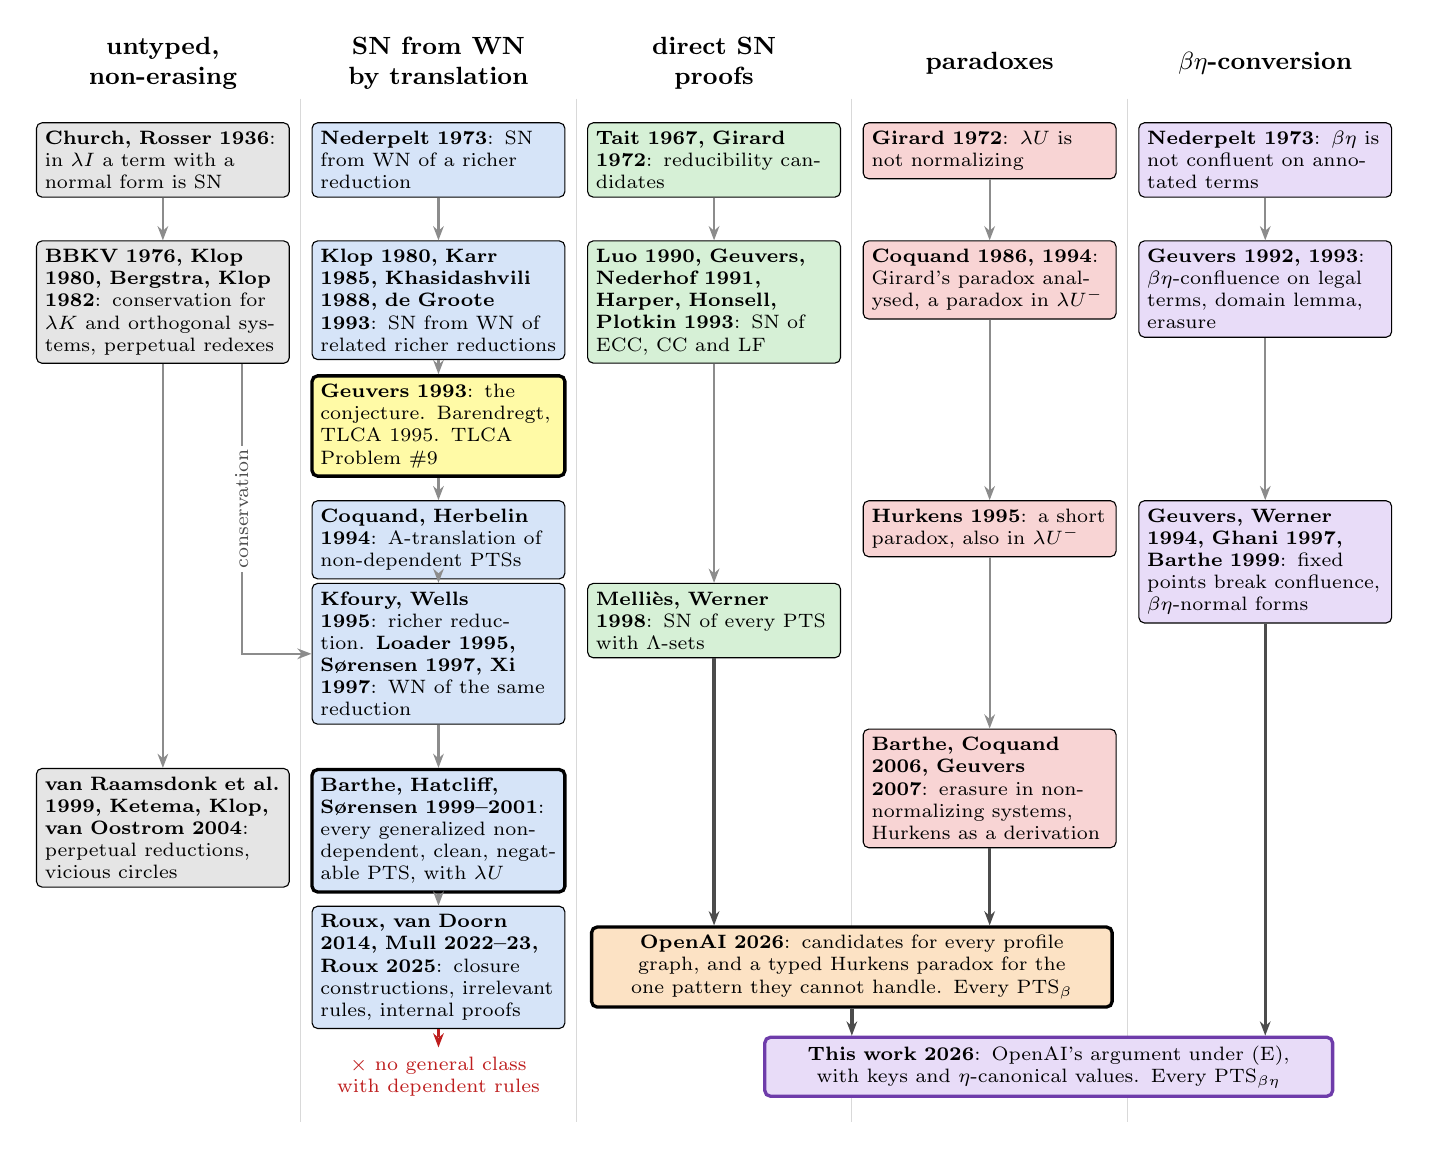
\begin{tikzpicture}[x=1cm,y=1cm,
  hb/.style={draw,rounded corners=2pt,align=left,font=\scriptsize,inner sep=3pt,
    text width=3.0cm,anchor=north},
  infl/.style={-{Stealth[length=1.8mm]},thick,black!45},
  lane/.style={font=\small\bfseries,align=center,text width=3.2cm}]
% Lane headers.
\node[lane] at (0,0.55) {untyped,\\ non-erasing};
\node[lane] at (3.5,0.55) {SN from WN\\ by translation};
\node[lane] at (7.0,0.55) {direct SN\\ proofs};
\node[lane] at (10.5,0.55) {paradoxes};
\node[lane] at (14.0,0.55) {$\beta\eta$-conversion};
\foreach \x in {1.75,5.25,8.75,12.25} \draw[black!15] (\x,0.1) -- (\x,-12.9);
% Untyped, non-erasing reduction.
\node[hb,fill=shared] (A1) at (0,-0.2)
  {\textbf{Church, Rosser 1936}: in $\lambda I$ a term with a normal form is SN};
\node[hb,fill=shared] (A2) at (0,-1.7)
  {\textbf{BBKV 1976, Klop 1980, Bergstra, Klop 1982}: conservation for $\lambda K$
   and orthogonal systems, perpetual redexes};
\node[hb,fill=shared] (A3) at (0,-8.4)
  {\textbf{van Raamsdonk et al.\ 1999, Ketema, Klop, van Oostrom 2004}: perpetual
   reductions, vicious circles};
% Translations.
\node[hb,fill=cand] (B1) at (3.5,-0.2)
  {\textbf{Nederpelt 1973}: SN from WN of a richer reduction};
\node[hb,fill=cand] (B2) at (3.5,-1.7)
  {\textbf{Klop 1980, Karr 1985, Khasidashvili 1988, de Groote 1993}: SN from WN of
   related richer reductions};
\node[hb,fill=yellow!35,very thick] (CJ) at (3.5,-3.4)
  {\textbf{Geuvers 1993}: the conjecture. Barendregt, TLCA 1995. TLCA
   Problem~\#9};
\node[hb,fill=cand] (B3) at (3.5,-5.0)
  {\textbf{Coquand, Herbelin 1994}: A-translation of non-dependent PTSs};
\node[hb,fill=cand] (B4) at (3.5,-6.05)
  {\textbf{Kfoury, Wells 1995}: richer reduction. \textbf{Loader 1995, Sørensen
   1997, Xi 1997}: WN of the same reduction};
\node[hb,fill=cand,very thick] (B5) at (3.5,-8.4)
  {\textbf{Barthe, Hatcliff, Sørensen 1999--2001}: every generalized non-dependent,
   clean, negatable PTS, with $\lambda U$};
\node[hb,fill=cand] (B6) at (3.5,-10.15)
  {\textbf{Roux, van Doorn 2014, Mull 2022--23, Roux 2025}: closure constructions,
   irrelevant rules, internal proofs};
\node[font=\scriptsize,text=warn,align=center,anchor=north] (stop) at (3.5,-11.95)
  {$\times$ no general class\\ with dependent rules};
% Direct proofs.
\node[hb,fill=easy] (C1) at (7.0,-0.2)
  {\textbf{Tait 1967, Girard 1972}: reducibility candidates};
\node[hb,fill=easy] (C2) at (7.0,-1.7)
  {\textbf{Luo 1990, Geuvers, Nederhof 1991, Harper, Honsell, Plotkin 1993}: SN of
   ECC, CC and LF};
\node[hb,fill=easy] (C3) at (7.0,-6.05)
  {\textbf{Melliès, Werner 1998}: SN of every PTS with $\Lambda$-sets};
% Paradoxes.
\node[hb,fill=par] (D1) at (10.5,-0.2)
  {\textbf{Girard 1972}: $\lambda U$ is not normalizing};
\node[hb,fill=par] (D2) at (10.5,-1.7)
  {\textbf{Coquand 1986, 1994}: Girard's paradox analysed, a paradox in $\lambda U^-$};
\node[hb,fill=par] (D3) at (10.5,-5.0)
  {\textbf{Hurkens 1995}: a short paradox, also in $\lambda U^-$};
\node[hb,fill=par] (D4) at (10.5,-7.9)
  {\textbf{Barthe, Coquand 2006, Geuvers 2007}: erasure in non-normalizing systems,
   Hurkens as a derivation};
% Beta-eta.
\node[hb,fill=etanew] (E1) at (14.0,-0.2)
  {\textbf{Nederpelt 1973}: $\beta\eta$ is not confluent on annotated terms};
\node[hb,fill=etanew] (E2) at (14.0,-1.7)
  {\textbf{Geuvers 1992, 1993}: $\beta\eta$-confluence on legal terms, domain
   lemma, erasure};
\node[hb,fill=etanew] (E3) at (14.0,-5.0)
  {\textbf{Geuvers, Werner 1994, Ghani 1997, Barthe 1999}: fixed points break
   confluence, $\beta\eta$-normal forms};
% The two proofs.
\node[hb,fill=obs,very thick,text width=6.4cm,align=center] (OAI) at (8.75,-10.4)
  {\textbf{OpenAI 2026}: candidates for every profile graph, and a typed Hurkens
   paradox for the one pattern they cannot handle. Every $\mathrm{PTS}_\beta$};
\node[hb,fill=etanew,draw=etaline,very thick,text width=7.0cm,align=center] (BE)
  at (11.25,-11.8)
  {\textbf{This work 2026}: OpenAI's argument under (E), with keys and
   $\eta$-canonical values. Every $\mathrm{PTS}_{\beta\eta}$};
% Influence.
\foreach \a/\b in {A1/A2,A2/A3,B1/B2,B2/CJ,CJ/B3,B3/B4,B4/B5,B5/B6,C1/C2,C2/C3,
                   D1/D2,D2/D3,D3/D4,E1/E2,E2/E3}
  \draw[infl] (\a) -- (\b);
\draw[infl] ([xshift=1cm]A2.south) |- node[pos=0.25,font=\scriptsize,rotate=90,
  fill=white,inner sep=1pt,text=black!70] {conservation} (B4.west);
\draw[infl,warn,dashed] (B6) -- (stop);
\draw[infl,very thick,black!70] (C3) -- (C3 |- OAI.north);
\draw[infl,very thick,black!70] (D4) -- (D4 |- OAI.north);
\draw[infl,very thick,black!70] (OAI.south) -- (OAI.south |- BE.north);
\draw[infl,very thick,black!70] (E3) -- (E3 |- BE.north);
\end{tikzpicture}
\caption{A genealogy of the proof. Columns are lines of work, rows run roughly
forward in time, and arrows indicate the use of earlier ideas. The translation line
(blue) derived SN from WN, but only up to non-dependent systems. OpenAI's proof
instead combines the reducibility method (green) with the paradoxes (red). Sources:
\cite{ChurchRosser1936,BBKV1976,Klop1980,BergstraKlop1982,vanRaamsdonkEtAl1999,
KetemaKlopvanOostrom2004,Nederpelt1973,Karr1985,Khasidashvili1988,deGroote1993,
Geuvers1993,TLCAProblem9,CoquandHerbelin1994,KfouryWells1995,Loader1995,
Sorensen1997IC,Xi1997,BHS1999,BartheHatcliffSorensen2001,RouxVanDoorn2014,
MullThunk2022,Mull2023,Roux2025,Tait1967,Girard1972,Luo1990,GeuversNederhof1991,
HarperHonsellPlotkin1993,MelliesWerner1998,Coquand1986,Coquand1994,Hurkens1995,
BartheCoquand2006,Geuvers2007,Geuvers1992,GeuversWerner1994,Ghani1997,Barthe1999,
OpenAI2026,PTSbetaetaLean}.}
\label{fig:genealogy}
\end{figure}

\paragraph{How close each line came.} Figure~\ref{fig:distance} measures the
distance to the conjecture along two axes. The vertical axis is the hypothesis. The
early techniques required weak normalization of a more complicated reduction, and
hence a new normalization proof for each calculus~\cite[Ch.~2]{Sorensen1997}. From
Sørensen onwards, the hypothesis is that of the conjecture. The horizontal axis is
the scope. Barthe, Hatcliff and Sørensen covered a uniform class that includes
non-normalizing systems such as $\lambda U$, and later work extended it
slightly~\cite{Mull2023,RouxVanDoorn2014}. None of these results reached a general
class with dependent rules.

\begin{figure}[H]
\centering
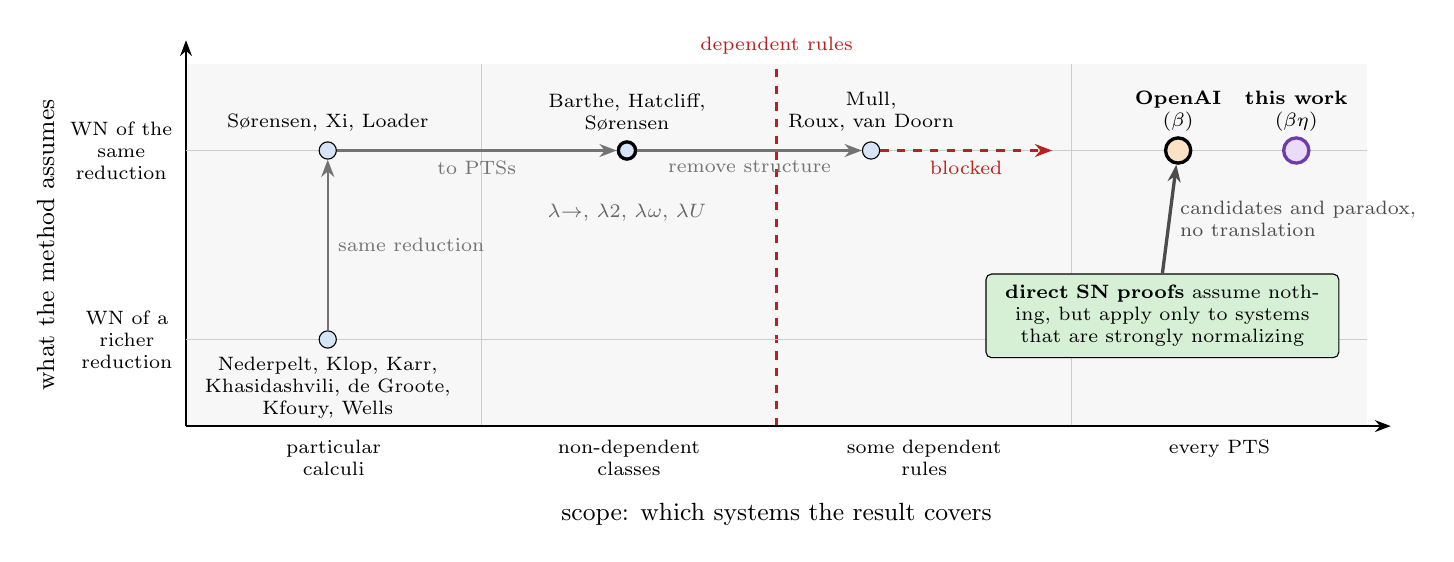
\begin{tikzpicture}[x=1cm,y=1cm,
  pt/.style={circle,draw,inner sep=2.2pt},
  plab/.style={font=\scriptsize,align=center}]
% Bands of scope.
\fill[black!3] (0,0) rectangle (15,4.6);
\foreach \x in {3.75,11.25} \draw[black!20] (\x,0) -- (\x,4.6);
\draw[warn,very thick,dashed] (7.5,0) -- (7.5,4.6);
\node[font=\scriptsize,text=warn,align=center,anchor=south] at (7.5,4.6)
  {dependent rules};
\draw[-{Stealth[length=2mm]},thick] (0,0) -- (15.3,0);
\draw[-{Stealth[length=2mm]},thick] (0,0) -- (0,4.9);
\node[font=\small,anchor=north] at (7.5,-0.85) {scope: which systems the result covers};
\node[font=\small,rotate=90,anchor=south] at (-1.55,2.3) {what the method assumes};
\node[plab,anchor=north] at (1.875,-0.05) {particular\\ calculi};
\node[plab,anchor=north] at (5.625,-0.05) {non-dependent\\ classes};
\node[plab,anchor=north] at (9.375,-0.05) {some dependent\\ rules};
\node[plab,anchor=north] at (13.125,-0.05) {every PTS};
\node[plab,anchor=east] at (-0.05,1.1) {WN of a\\ richer\\ reduction};
\node[plab,anchor=east] at (-0.05,3.5) {WN of the\\ same\\ reduction};
\draw[black!20] (0,1.1) -- (15,1.1);
\draw[black!20] (0,3.5) -- (15,3.5);
% Results.
\node[pt,fill=cand] (p1) at (1.8,1.1) {};
\node[plab,anchor=north] at (1.8,1.0) {Nederpelt, Klop, Karr,\\ Khasidashvili, de Groote,\\ Kfoury, Wells};
\node[pt,fill=cand] (p2) at (1.8,3.5) {};
\node[plab,anchor=south] at (1.8,3.62) {Sørensen, Xi, Loader};
\node[pt,fill=cand,very thick] (p3) at (5.6,3.5) {};
\node[plab,anchor=south] at (5.6,3.62) {Barthe, Hatcliff,\\ Sørensen};
\node[plab,anchor=north,text=black!60] at (5.6,2.95) {$\lambda{\to}$, $\lambda2$, $\lambda\omega$, $\lambda U$};
\node[pt,fill=cand] (p4) at (8.7,3.5) {};
\node[plab,anchor=south] at (8.7,3.62) {Mull,\\ Roux, van Doorn};
\node[pt,fill=obs,very thick,minimum size=3.2mm] (p5) at (12.6,3.5) {};
\node[plab,anchor=south] at (12.6,3.62) {\textbf{OpenAI}\\ ($\beta$)};
\node[pt,fill=etanew,draw=etaline,very thick,minimum size=3.2mm] (p6) at (14.1,3.5) {};
\node[plab,anchor=south] at (14.1,3.62) {\textbf{this work}\\ ($\beta\eta$)};
\draw[arr,black!55] (p1) -- node[plab,right] {same reduction} (p2);
\draw[arr,black!55] (p2) -- node[plab,below] {to PTSs} (p3);
\draw[arr,black!55] (p3) -- node[plab,below] {remove structure} (p4);
\draw[arr,warn,dashed] (p4) -- node[plab,below,text=warn] {blocked} (11.0,3.5);
% Direct proofs and the route of OpenAI.
\node[box,fill=easy,text width=4.2cm,font=\scriptsize] (dir) at (12.4,1.4)
  {\textbf{direct SN proofs} assume nothing, but apply only to systems that are
   strongly normalizing};
\draw[arr,black!70,very thick] (dir.north) -- node[plab,right,align=left]
  {candidates and paradox,\\ no translation} (p5);
\end{tikzpicture}
\caption{How close each result came to the conjecture, shown qualitatively. The red
line marks dependent rules, where every translation result stops, because
translating a term first requires translating its type. OpenAI reaches every system
from a different direction, starting from the reducibility method of direct proofs.
The systems listed under Barthe, Hatcliff and Sørensen are examples from their
class.}
\label{fig:distance}
\end{figure}

\paragraph{Two routes.} Figure~\ref{fig:routes} shows why the translation route
needs particular rules while the new route does not. A translation must type
$\llbracket M\rrbracket$ in the same system. A negation requires a rule $(s,s,s)$,
and in the presence of dependency, translating a term requires translating its type,
which may be larger~\cite[\S3.6]{Sorensen1997}. OpenAI's route builds candidates
directly and uses weak normalization only to obtain normal forms and, once, against
the paradox.

\begin{figure}[H]
\centering
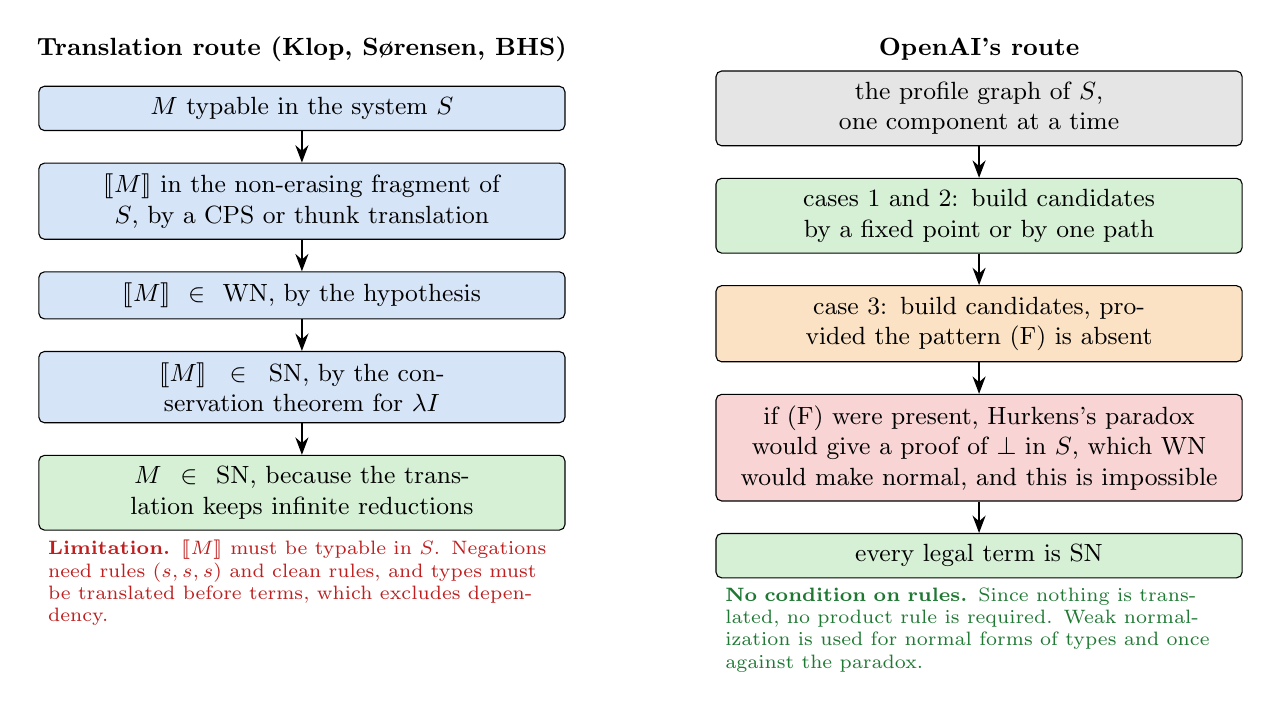
\begin{tikzpicture}[x=1cm,y=1cm,node distance=4mm,
  rb/.style={box,text width=6.4cm,font=\small}]
\begin{scope}
\node[font=\small\bfseries] at (0,0.75) {Translation route (Klop, Sørensen, BHS)};
\node[rb,fill=cand] (t1) at (0,0) {$M$ typable in the system $S$};
\node[rb,fill=cand,below=of t1] (t2)
  {$\llbracket M\rrbracket$ in the non-erasing fragment of $S$, by a CPS or thunk
   translation};
\node[rb,fill=cand,below=of t2] (t3) {$\llbracket M\rrbracket\in\mathrm{WN}$, by the
  hypothesis};
\node[rb,fill=cand,below=of t3] (t4) {$\llbracket M\rrbracket\in\mathrm{SN}$, by the
  conservation theorem for $\lambda I$};
\node[rb,fill=easy,below=of t4] (t5) {$M\in\mathrm{SN}$, because the translation
  keeps infinite reductions};
\foreach \a/\b in {t1/t2,t2/t3,t3/t4,t4/t5} \draw[arr] (\a) -- (\b);
\node[font=\scriptsize,text=warn,align=left,anchor=north west,text width=6.4cm]
  at (t5.south west)
  {\textbf{Limitation.} $\llbracket M\rrbracket$ must be typable in $S$. Negations
   need rules $(s,s,s)$ and clean rules, and types must be translated before terms,
   which excludes dependency.};
\end{scope}
\begin{scope}[xshift=8.6cm]
\node[font=\small\bfseries] at (0,0.75) {OpenAI's route};
\node[rb,fill=shared] (o1) at (0,0) {the profile graph of $S$, one component at a
  time};
\node[rb,fill=easy,below=of o1] (o2) {cases 1 and 2: build candidates by a fixed
  point or by one path};
\node[rb,fill=obs,below=of o2] (o3) {case 3: build candidates, provided the
  pattern (F) is absent};
\node[rb,fill=par,below=of o3] (o4) {if (F) were present, Hurkens's paradox would
  give a proof of $\bot$ in $S$, which WN would make normal, and this is impossible};
\node[rb,fill=easy,below=of o4] (o5) {every legal term is SN};
\foreach \a/\b in {o1/o2,o2/o3,o3/o4,o4/o5} \draw[arr] (\a) -- (\b);
\node[font=\scriptsize,text=okgreen,align=left,anchor=north west,text width=6.4cm]
  at (o5.south west)
  {\textbf{No condition on rules.} Since nothing is translated, no product rule is
   required. Weak normalization is used for normal forms of types and once against
   the paradox.};
\end{scope}
\end{tikzpicture}
\caption{The mechanism of the strongest earlier results (left) and of OpenAI's proof
(right). The left route requires suitable product rules inside the system, and the
right route requires none.}
\label{fig:routes}
\end{figure}

\clearpage
%======================================================================
\section{The \texorpdfstring{$\beta$}{beta} proof}\label{sec:whole}

\begin{figure}[H]
\centering
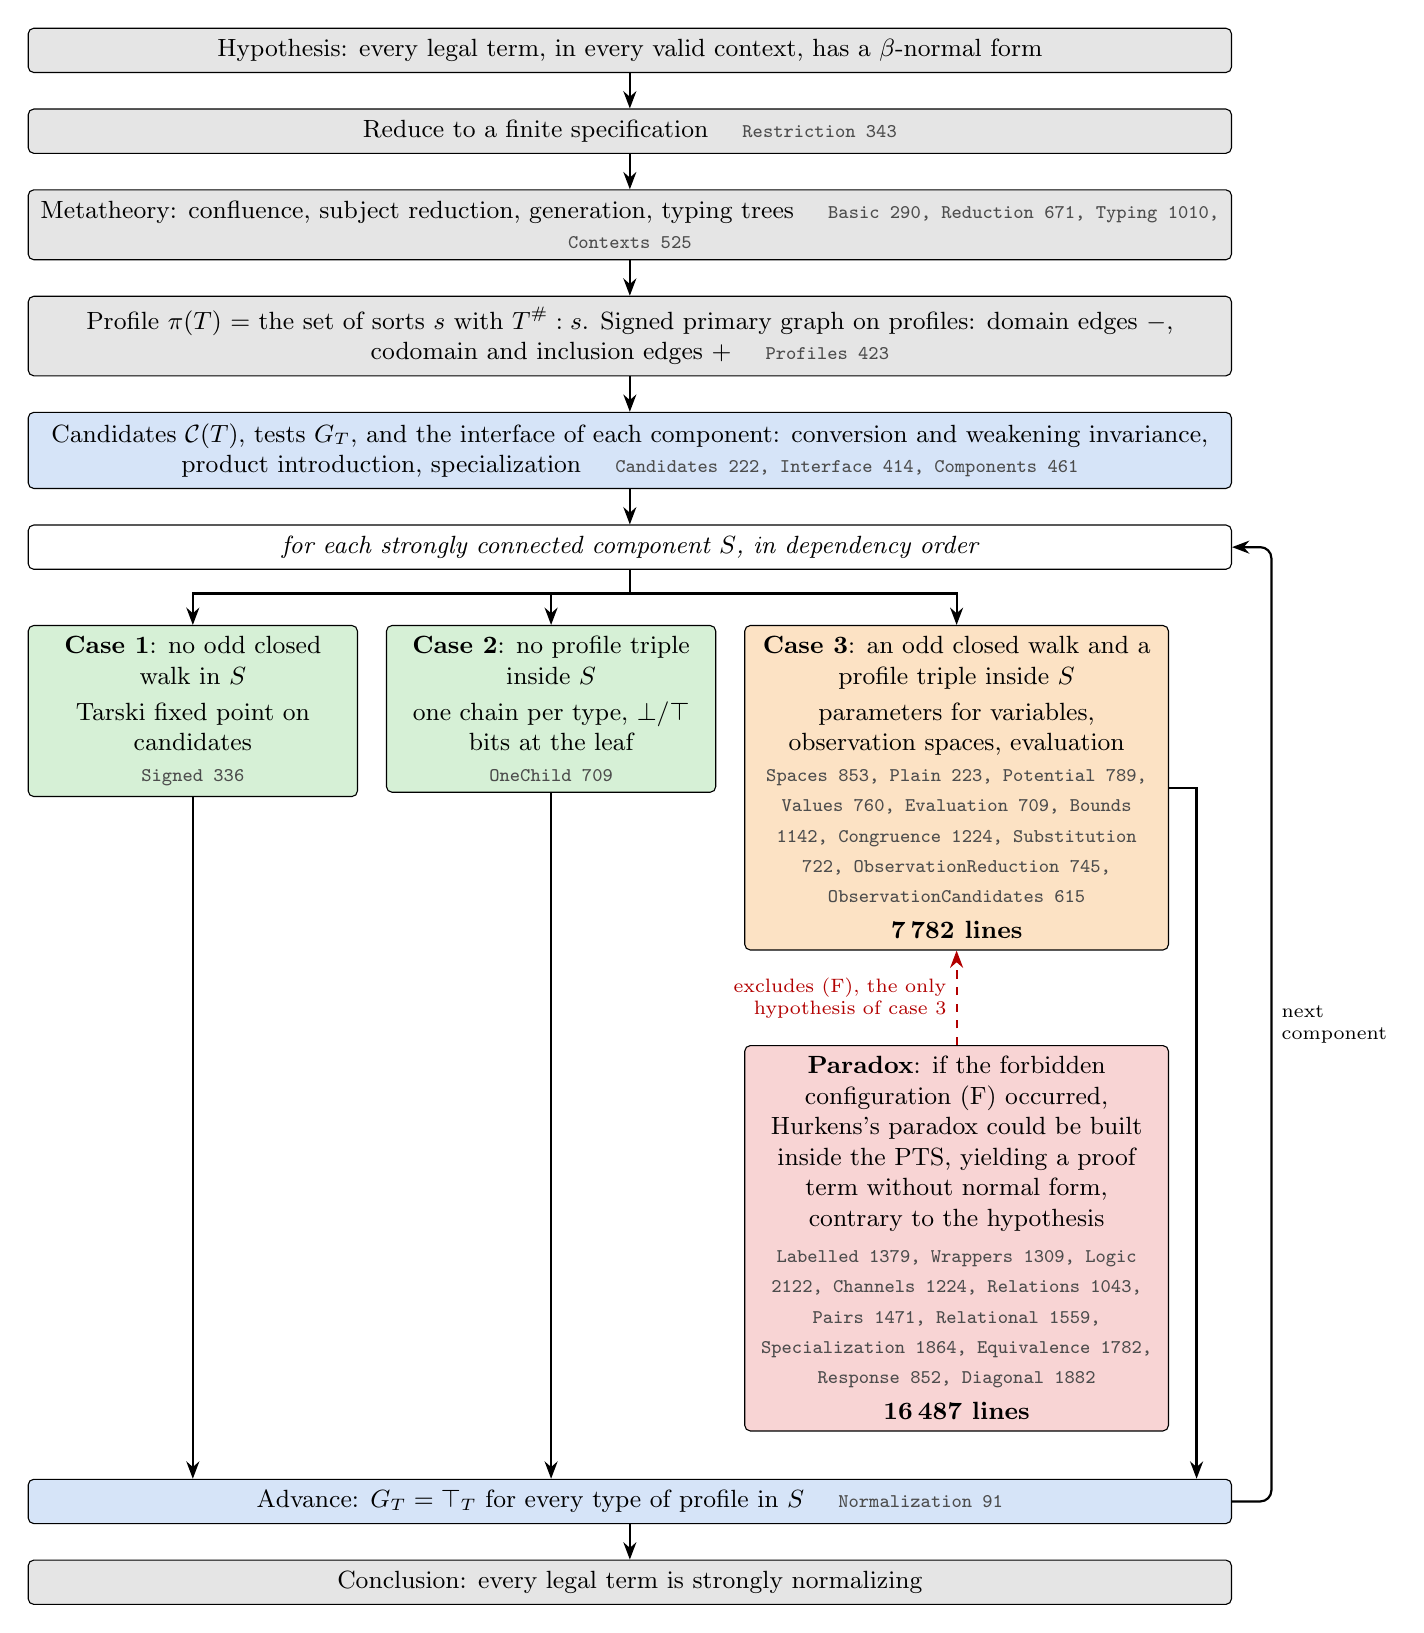
\begin{tikzpicture}[node distance=4.5mm,box/.append style={align=flush center}]
\node[box,fill=shared,text width=15cm] (wn)
  {Hypothesis: every legal term, in every valid context, has a $\beta$-normal form};
\node[box,fill=shared,text width=15cm,below=of wn] (fin)
  {Reduce to a finite specification \quad
   {\lean Restriction 343}};
\node[box,fill=shared,text width=15cm,below=of fin] (meta)
  {Metatheory: confluence, subject reduction, generation, typing trees \quad
   {\lean Basic 290, Reduction 671, Typing 1010, Contexts 525}};
\node[box,fill=shared,text width=15cm,below=of meta] (prof)
  {Profile $\pi(T)$ = the set of sorts $s$ with $T^\#:s$.
   Signed primary graph on profiles: domain edges $-$, codomain and inclusion edges $+$
   \quad {\lean Profiles 423}};
\node[box,fill=cand,text width=15cm,below=of prof] (cand)
  {Candidates $\mathcal C(T)$, tests $G_T$, and the interface of each component:
   conversion and weakening invariance, product introduction, specialization \quad
   {\lean Candidates 222, Interface 414, Components 461}};
\node[box,fill=white,text width=15cm,below=of cand,font=\small\itshape] (loop)
  {for each strongly connected component $S$, in dependency order};
\coordinate (row) at ($(loop.south)+(0,-7mm)$);
\node[box,fill=easy,text width=3.9cm,anchor=north] (c1) at (row -| -5.55,0)
  {\textbf{Case 1}: no odd closed walk in $S$\\[2pt]
   Tarski fixed point on candidates\\ {\lean Signed 336}};
\node[box,fill=easy,text width=3.9cm,anchor=north] (c2) at (row -| -1.00,0)
  {\textbf{Case 2}: no profile triple inside $S$\\[2pt]
   one chain per type, $\bot$/$\top$ bits at the leaf\\ {\lean OneChild 709}};
\node[box,fill=obs,text width=5.1cm,anchor=north] (c3) at (row -| 4.15,0)
  {\textbf{Case 3}: an odd closed walk and a profile triple inside $S$\\[2pt]
   parameters for variables, observation spaces, evaluation\\
   {\lean Spaces 853, Plain 223, Potential 789, Values 760, Evaluation 709,
   Bounds 1142, Congruence 1224, Substitution 722, ObservationReduction 745,
   ObservationCandidates 615}\\[2pt] \textbf{7\,782 lines}};
\node[box,fill=par,text width=5.1cm,below=12mm of c3] (par)
  {\textbf{Paradox}: if the forbidden configuration (F) occurred, Hurkens's
   paradox could be built inside the PTS, yielding a proof term without normal
   form, contrary to the hypothesis\\[2pt]
   {\lean Labelled 1379, Wrappers 1309, Logic 2122, Channels 1224, Relations 1043,
   Pairs 1471, Relational 1559, Specialization 1864, Equivalence 1782,
   Response 852, Diagonal 1882}\\[2pt] \textbf{16\,487 lines}};
\coordinate (low) at ($(par.south)+(0,-6mm)$);
\node[box,fill=cand,text width=15cm,anchor=north] (adv) at (low -| loop)
  {Advance: $G_T=\top_T$ for every type of profile in $S$ \quad {\lean Normalization 91}};
\node[box,fill=shared,text width=15cm,below=of adv] (sn)
  {Conclusion: every legal term is strongly normalizing};

\foreach \a/\b in {wn/fin,fin/meta,meta/prof,prof/cand,cand/loop,adv/sn}
  \draw[arr] (\a) -- (\b);
\draw[arr] (loop.south) -- ++(0,-3mm) -| (c1.north);
\draw[arr] (loop.south) -- ++(0,-3mm) -| (c2.north);
\draw[arr] (loop.south) -- ++(0,-3mm) -| (c3.north);
\draw[arr,dashed,red!70!black] (par.north) -- node[left,font=\scriptsize,align=right]
  {excludes (F), the only\\ hypothesis of case 3} (c3.south);
\draw[arr] (c1.south) -- (c1.south |- adv.north);
\draw[arr] (c2.south) -- (c2.south |- adv.north);
\draw[arr] (c3.east) -- ++(0.35,0) coordinate (bend) -- (bend |- adv.north);
\draw[arr,rounded corners] (adv.east) -- ++(0.5,0) |- (loop.east)
  node[pos=0.25,right,font=\scriptsize,align=left] {next\\ component};
\end{tikzpicture}
\caption{OpenAI's proof and its Lean files, with line counts from the copy in
\texttt{PTS-beta-eta/PTSBetaEta/Beta} (29\,764 lines in total). Gray marks ordinary
PTS metatheory, blue the candidate method, green and orange the three constructions,
and red the paradox. The paradox makes up 55\% of the code and serves only to
exclude one finite graph pattern.}
\label{fig:map}
\end{figure}

\clearpage
%======================================================================
\section{Candidates and why they are hard to build}\label{sec:equation}

At each actual type $T$ the proof works with three sets of terms
(Figure~\ref{fig:tests}). The set $\top_T$ consists of the typed strongly
normalizing terms, the set $G_T$ consists of the terms that remain strongly
normalizing under every stack of tested arguments, and a candidate is a set lying
between the two. The theorem follows once $G_T=\top_T$ is proved for every type.

\begin{figure}[H]
\centering
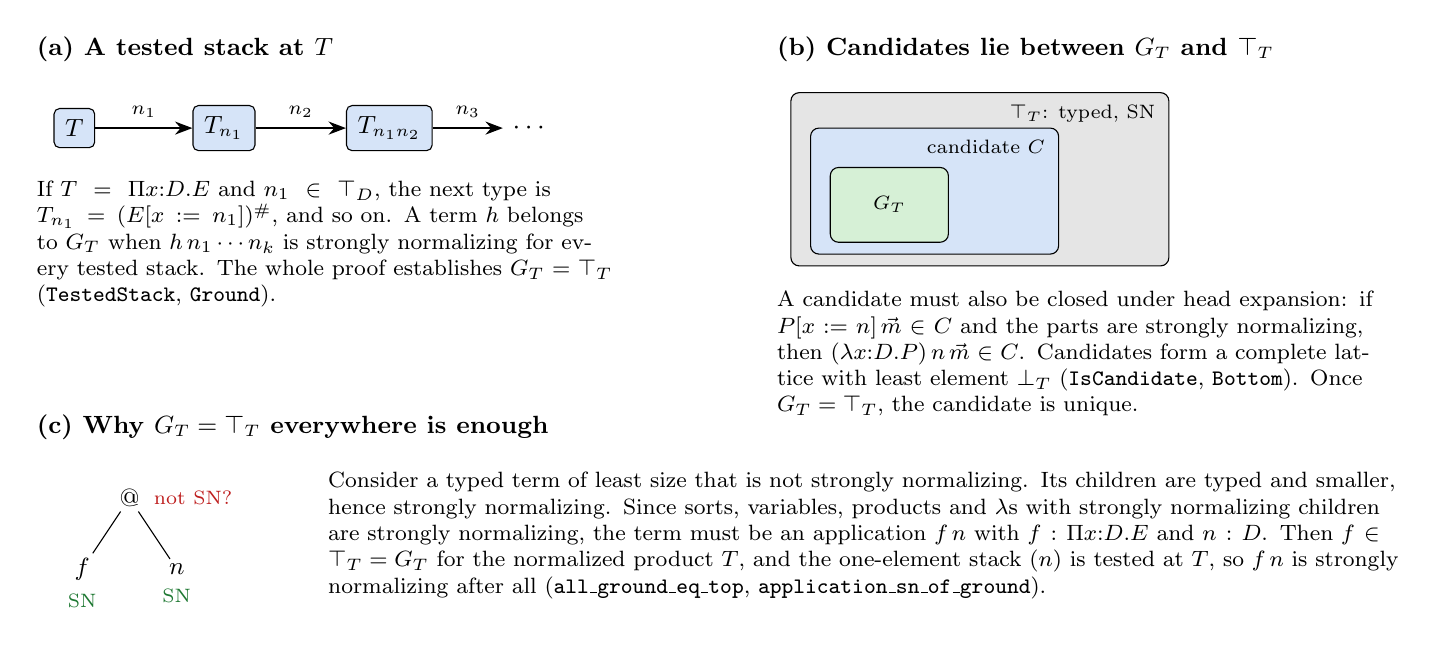
\begin{tikzpicture}[x=1cm,y=1cm]
% (a) A tested stack.
\node[font=\small\bfseries,anchor=west] at (-0.3,1.0) {(a) A tested stack at $T$};
\node[box,fill=cand] (T0) at (0.3,0) {$T$};
\node[box,fill=cand] (T1) at (2.2,0) {$T_{n_1}$};
\node[box,fill=cand] (T2) at (4.3,0) {$T_{n_1n_2}$};
\node (T3) at (6.1,0) {$\cdots$};
\draw[arr] (T0) -- node[lbl,above] {$n_1$} (T1);
\draw[arr] (T1) -- node[lbl,above] {$n_2$} (T2);
\draw[arr] (T2) -- node[lbl,above] {$n_3$} (T3);
\node[expl,text width=7.4cm] at (-0.3,-0.55)
  {If $T=\Pi x{:}D.E$ and $n_1\in\top_D$, the next type is $T_{n_1}=(E[x:=n_1])^\#$,
   and so on. A term $h$ belongs to $G_T$ when $h\,n_1\cdots n_k$ is strongly
   normalizing for every tested stack. The whole proof establishes $G_T=\top_T$
   (\texttt{TestedStack}, \texttt{Ground}).};
% (b) Candidates.
\begin{scope}[xshift=9.4cm]
\node[font=\small\bfseries,anchor=west] at (-0.3,1.0)
  {(b) Candidates lie between $G_T$ and $\top_T$};
\draw[rounded corners=3pt,fill=shared] (0,-1.75) rectangle (4.8,0.45);
\draw[rounded corners=3pt,fill=cand] (0.25,-1.6) rectangle (3.4,0.0);
\draw[rounded corners=3pt,fill=easy] (0.5,-1.45) rectangle (2.0,-0.5);
\node[lbl,anchor=north east] at (4.75,0.42) {$\top_T$: typed, SN};
\node[lbl,anchor=north east] at (3.35,-0.03) {candidate $C$};
\node[lbl] at (1.25,-0.97) {$G_T$};
\node[expl,text width=7.6cm] at (-0.3,-1.95)
  {A candidate must also be closed under head expansion: if $P[x:=n]\,\vec m\in C$
   and the parts are strongly normalizing, then $(\lambda x{:}D.P)\,n\,\vec m\in C$.
   Candidates form a complete lattice with least element $\bot_T$
   (\texttt{IsCandidate}, \texttt{Bottom}). Once $G_T=\top_T$, the candidate is
   unique.};
\end{scope}
% (c) Why the invariant suffices.
\begin{scope}[yshift=-4.7cm]
\node[font=\small\bfseries,anchor=west] at (-0.3,0.9)
  {(c) Why $G_T=\top_T$ everywhere is enough};
\node[tn] (ap) at (1.0,0) {$@$};
\node[tn] (ff) at (0.4,-0.9) {$f$};
\node[tn] (nn) at (1.6,-0.9) {$n$};
\draw (ap) -- (ff); \draw (ap) -- (nn);
\node[lbl,text=okgreen,anchor=north] at (ff.south) {SN};
\node[lbl,text=okgreen,anchor=north] at (nn.south) {SN};
\node[lbl,text=warn,anchor=west] at (ap.east) {not SN?};
\node[expl,text width=13.6cm] at (3.4,0.45)
  {Consider a typed term of least size that is not strongly normalizing. Its children
   are typed and smaller, hence strongly normalizing. Since sorts, variables, products
   and $\lambda$s with strongly normalizing children are strongly normalizing, the
   term must be an application $f\,n$ with $f:\Pi x{:}D.E$ and $n:D$. Then
   $f\in\top_T=G_T$ for the normalized product $T$, and the one-element stack $(n)$ is
   tested at $T$, so $f\,n$ is strongly normalizing after all
   (\texttt{all\_ground\_eq\_top}, \texttt{application\_sn\_of\_ground}).};
\end{scope}
\end{tikzpicture}
\caption{The objects of the candidate method. (a)~Tests follow the exact successive
types. (b)~A candidate is any set between the tests and the typed strongly
normalizing terms that is closed under head expansion. (c)~The invariant
$G_T=\top_T$ for every type rules out a smallest counterexample.}
\label{fig:tests}
\end{figure}

Every construction in the proof solves the same equation. For a type
$T=\Pi x{:}D.E$ whose profile lies in the current component, the candidate of
$T$ must be the set of strongly normalizing terms that map good arguments to good
results:
\[
  R\bigl(\Pi x{:}D.E\bigr)\;=\;\bigl\{\,h\in\mathrm{SN}\;:\;
     h\,n\in R\bigl((E[x:=n])^\#\bigr)\ \text{for every } n\in R(D)\,\bigr\}.
\]
This is Girard's equation for reducibility candidates~\cite{Girard1989}. In
System~F it is solved by recursion on the type, but in a general PTS three obstacles
prevent this recursion.

\begin{figure}[H]
\centering
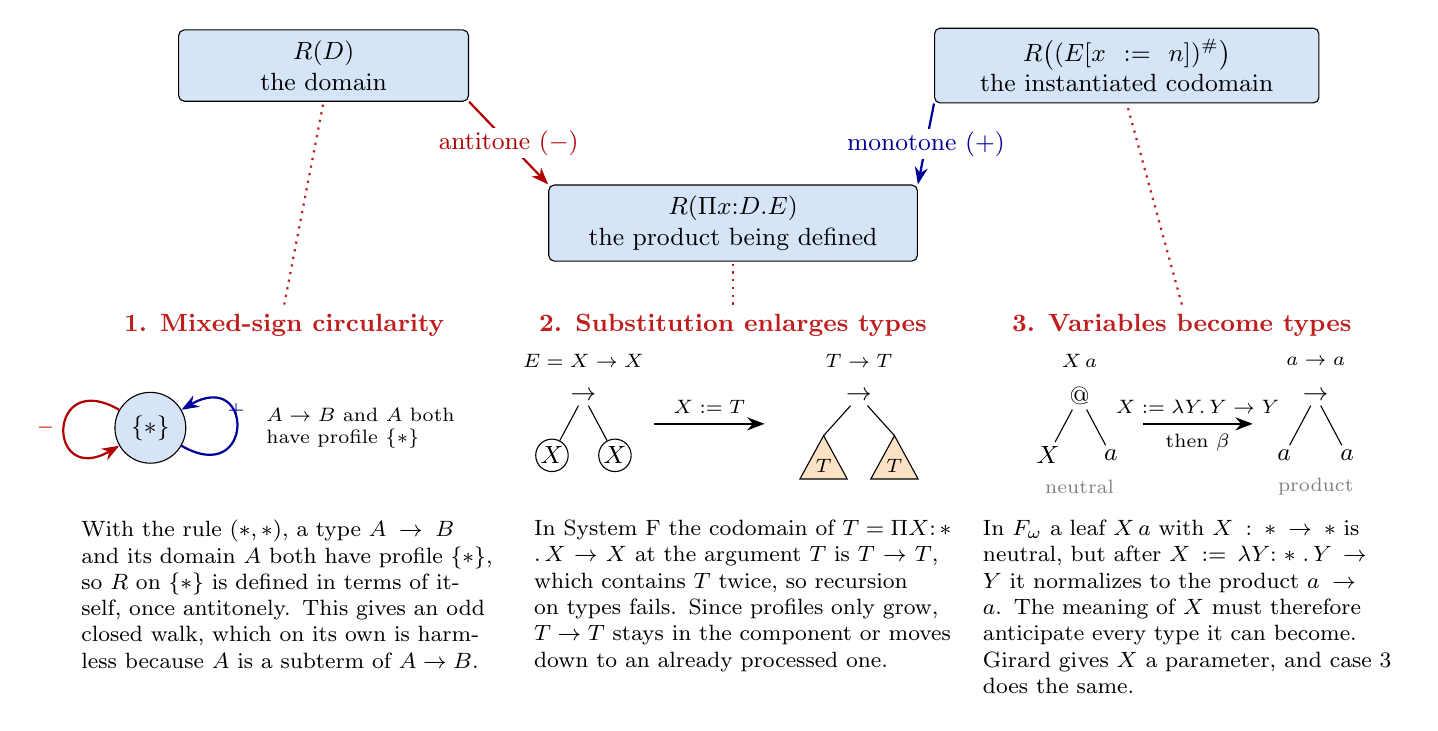
\begin{tikzpicture}
\node[box,fill=cand,text width=4.4cm] (T) at (0,0)
  {$R(\Pi x{:}D.E)$\\ the product being defined};
\node[box,fill=cand,text width=3.4cm] (D) at (-5.2,2.0) {$R(D)$\\ the domain};
\node[box,fill=cand,text width=4.6cm] (E) at (5.0,2.0)
  {$R\bigl((E[x:=n])^\#\bigr)$\\ the instantiated codomain};
\draw[negedge] (D.south east) -- node[midway,fill=white,inner sep=1pt,font=\small]
  {antitone ($-$)} (T.north west);
\draw[posedge] (E.south west) -- node[midway,fill=white,inner sep=1pt,font=\small]
  {monotone ($+$)} (T.north east);

% Panel titles, linked to the part of the equation they concern.
\node[font=\small\bfseries,text=warn] (o1) at (-5.7,-1.3) {1. Mixed-sign circularity};
\node[font=\small\bfseries,text=warn] (o2) at (0,-1.3) {2. Substitution enlarges types};
\node[font=\small\bfseries,text=warn] (o3) at (5.7,-1.3) {3. Variables become types};
\draw[warn,thick,dotted] (o1.north) -- (D.south);
\draw[warn,thick,dotted] (o2.north) -- (T.south);
\draw[warn,thick,dotted] (o3.north) -- (E.south);
% Panel 1. A layer whose products have domains in the same layer.
\node[v,fill=cand] (st) at (-7.4,-2.6) {$\{*\}$};
\draw[negedge] (st) to[out=150,in=210,looseness=6] node[lbl,left] {$-$} (st);
\draw[posedge] (st) to[out=-30,in=30,looseness=6] node[lbl,above] {$+$} (st);
\node[lbl,align=left,anchor=west] at (-6.05,-2.6) {$A\to B$ and $A$ both\\ have profile $\{*\}$};
% Panel 2. System F: the codomain of T at the argument T contains T twice.
\node[lbl] at (-1.9,-1.75) {$E=X\to X$};
\node[tn] (e) at (-1.9,-2.2) {$\to$};
\node[tn,circle,draw,inner sep=0.5pt] (e1) at (-2.3,-2.95) {$X$};
\node[tn,circle,draw,inner sep=0.5pt] (e2) at (-1.5,-2.95) {$X$};
\draw (e) -- (e1); \draw (e) -- (e2);
\draw[arr] (-1.0,-2.55) -- node[lbl,above] {$X:=T$} (0.4,-2.55);
\node[lbl] at (1.6,-1.75) {$T\to T$};
\node[tn] (r) at (1.6,-2.2) {$\to$};
\draw[fill=obs] (0.85,-3.25) -- (1.15,-2.7) -- (1.45,-3.25) -- cycle;
\draw[fill=obs] (1.75,-3.25) -- (2.05,-2.7) -- (2.35,-3.25) -- cycle;
\node[lbl] at (1.15,-3.08) {$T$};
\node[lbl] at (2.05,-3.08) {$T$};
\draw (r) -- (1.15,-2.7); \draw (r) -- (2.05,-2.7);
% Panel 3. F-omega: a neutral leaf turns into a product.
\node[lbl] at (4.4,-1.75) {$X\,a$};
\node[tn] (l) at (4.4,-2.2) {$@$};
\node[tn] (lX) at (4.0,-2.95) {$X$};
\node[tn] (la) at (4.8,-2.95) {$a$};
\draw (l) -- (lX); \draw (l) -- (la);
\draw[arr] (5.2,-2.55) -- node[lbl,above] {$X:=\lambda Y.\,Y\to Y$}
  node[lbl,below] {then $\beta$} (6.6,-2.55);
\node[lbl] at (7.4,-1.75) {$a\to a$};
\node[tn] (p) at (7.4,-2.2) {$\to$};
\node[tn] (pa1) at (7.0,-2.95) {$a$};
\node[tn] (pa2) at (7.8,-2.95) {$a$};
\draw (p) -- (pa1); \draw (p) -- (pa2);
\node[lbl,text=black!50] at (4.4,-3.35) {neutral};
\node[lbl,text=black!50] at (7.4,-3.35) {product};
% Explanations.
\node[expl,text width=5.3cm] at (-8.4,-3.65)
  {With the rule $(*,*)$, a type $A\to B$ and its domain $A$ both have profile
   $\{*\}$, so $R$ on $\{*\}$ is defined in terms of itself, once antitonely. This
   gives an odd closed walk, which on its own is harmless because $A$ is a subterm of
   $A\to B$.};
\node[expl,text width=5.3cm] at (-2.65,-3.65)
  {In System~F the codomain of $T=\Pi X{:}*.\,X\to X$ at the argument $T$ is $T\to T$,
   which contains $T$ twice, so recursion on types fails. Since profiles only grow,
   $T\to T$ stays in the component or moves down to an already processed one.};
\node[expl,text width=5.3cm] at (3.05,-3.65)
  {In $F_\omega$ a leaf $X\,a$ with $X:*\to*$ is neutral, but after
   $X:=\lambda Y{:}*.\,Y\to Y$ it normalizes to the product $a\to a$. The meaning of
   $X$ must therefore anticipate every type it can become. Girard gives $X$ a
   parameter, and case~3 does the same.};
\end{tikzpicture}
\caption{The equation behind every candidate construction and its three obstacles,
shown on familiar systems. Case~1 removes obstacle~1 through sign consistency, and
case~2 removes obstacles~2 and~3 through structure. Case~3 faces all three, at the
cost of observation spaces and the paradox.}
\label{fig:equation}
\end{figure}

\section{The three cases}\label{sec:pattern}

The case split applies the same test twice, once to candidates and once to the
parameter spaces that case~3 introduces. At each level the proof asks two questions
about the dependency graph of the definitions it has to make.
\begin{enumerate}
\item \textbf{Are the signs consistent?} If every closed walk is even, each vertex
  can be given a sign. The definition then becomes monotone in a mixed order and has
  an order-theoretic fixed point. For candidates this is Tarski's
  theorem~\cite{Tarski1955} (case~1), and for parameter spaces it is the alternating
  chain $C_0=\emptyset$, $P_r=\mathrm{Tab}(C_r)$, $C_{r+1}=\mathrm{Tab}(P_r)$ (free
  layers).
\item \textbf{Does a measure decrease?} If every dependency points to something
  smaller, the definition can be made by recursion. For candidates the measure is
  the syntax of a single chain, which exists when no product has two children in
  the component (case~2). For parameter spaces it is the count $p_C$ of nodes along
  the component (plain layers).
\item \textbf{Neither.} At the candidate level the proof moves up one level and adds
  parameters (case~3). At the level of spaces there is no further level to move to.
  The proof shows that this situation, the \emph{forbidden configuration}, allows
  the system to encode Hurkens's paradox~\cite{Hurkens1995}, so it cannot occur in a
  weakly normalizing system.
\end{enumerate}
This mirrors the familiar trichotomy for recursive type definitions: positive or
sign-consistent definitions have solutions, decreasing definitions have solutions,
and a definition that is both negative and non-decreasing leads to a Russell-style
paradox. The proof turns this third alternative into a contradiction with weak
normalization.

\begin{figure}[H]
\centering
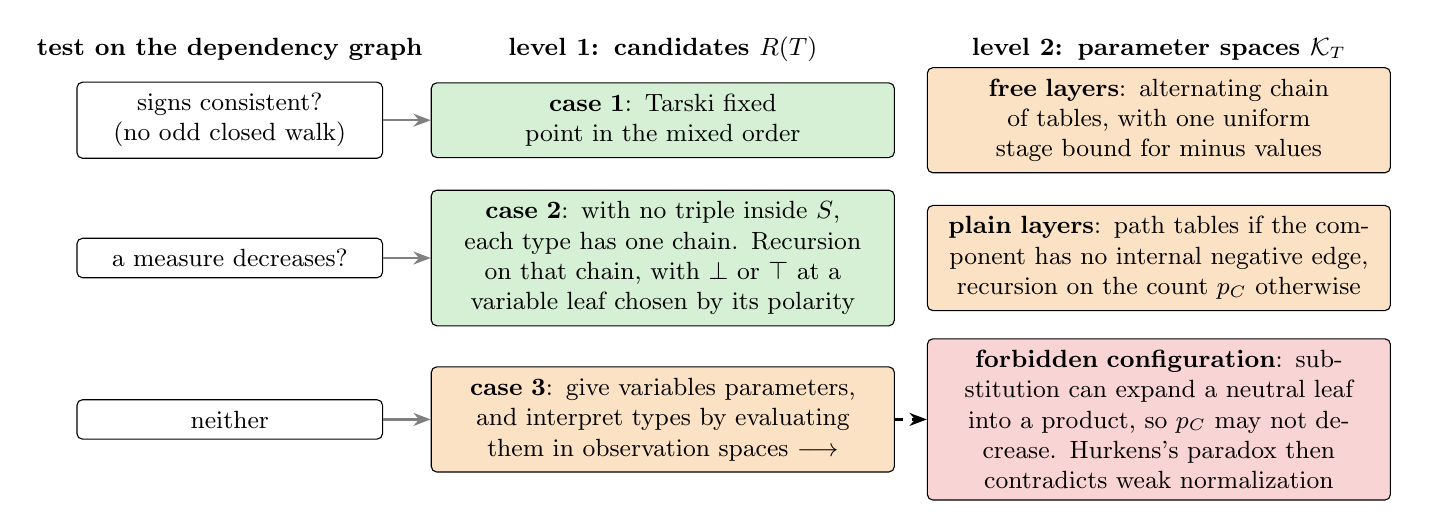
\begin{tikzpicture}[x=1cm,y=1cm]
\node[font=\small\bfseries] at (-0.2,0.9) {test on the dependency graph};
\node[font=\small\bfseries,text width=6cm,align=center] at (5.3,0.9)
  {level 1: candidates $R(T)$};
\node[font=\small\bfseries,text width=6cm,align=center] at (11.6,0.9)
  {level 2: parameter spaces $\mathcal K_T$};

\node[box,text width=3.6cm,fill=white] (q1) at (-0.2,0) {signs consistent?\\ (no odd closed walk)};
\node[box,text width=3.6cm,fill=white] (q2) at (-0.2,-1.75) {a measure decreases?};
\node[box,text width=3.6cm,fill=white] (q3) at (-0.2,-3.8) {neither};

\node[box,fill=easy,text width=5.6cm] (a1) at (5.3,0)
  {\textbf{case 1}: Tarski fixed point in the mixed order};
\node[box,fill=easy,text width=5.6cm] (a2) at (5.3,-1.75)
  {\textbf{case 2}: with no triple inside $S$, each type has one chain.
   Recursion on that chain, with $\bot$ or $\top$ at a variable leaf
   chosen by its polarity};
\node[box,fill=obs,text width=5.6cm] (a3) at (5.3,-3.8)
  {\textbf{case 3}: give variables parameters, and interpret types by
   evaluating them in observation spaces $\longrightarrow$};

\node[box,fill=obs,text width=5.6cm] (b1) at (11.6,0)
  {\textbf{free layers}: alternating chain of tables, with one uniform
   stage bound for minus values};
\node[box,fill=obs,text width=5.6cm] (b2) at (11.6,-1.75)
  {\textbf{plain layers}: path tables if the component has no internal
   negative edge, recursion on the count $p_C$ otherwise};
\node[box,fill=par,text width=5.6cm] (b3) at (11.6,-3.8)
  {\textbf{forbidden configuration}: substitution can expand a neutral leaf
   into a product, so $p_C$ may not decrease. Hurkens's paradox then
   contradicts weak normalization};

\foreach \i in {1,2,3} { \draw[arr,gray] (q\i) -- (a\i); }
\draw[arr,dashed] (a3.east) -- (b3.west);
\end{tikzpicture}
\caption{One test applied at two levels. Each row is one way of solving the
equation of Figure~\ref{fig:equation}. Only the bottom right cell is impossible,
and the paradox shows that it never arises under weak normalization.}
\label{fig:pattern}
\end{figure}

\paragraph{The two simple constructions.} Figure~\ref{fig:case12} illustrates
cases~1 and~2 on examples. Case~1 needs no syntax at all, since it works on the set
of all actual types of the component at once. Case~2 uses syntax, but only one path
in each type, and it never looks inside a type produced by substitution.

\begin{figure}[H]
\centering
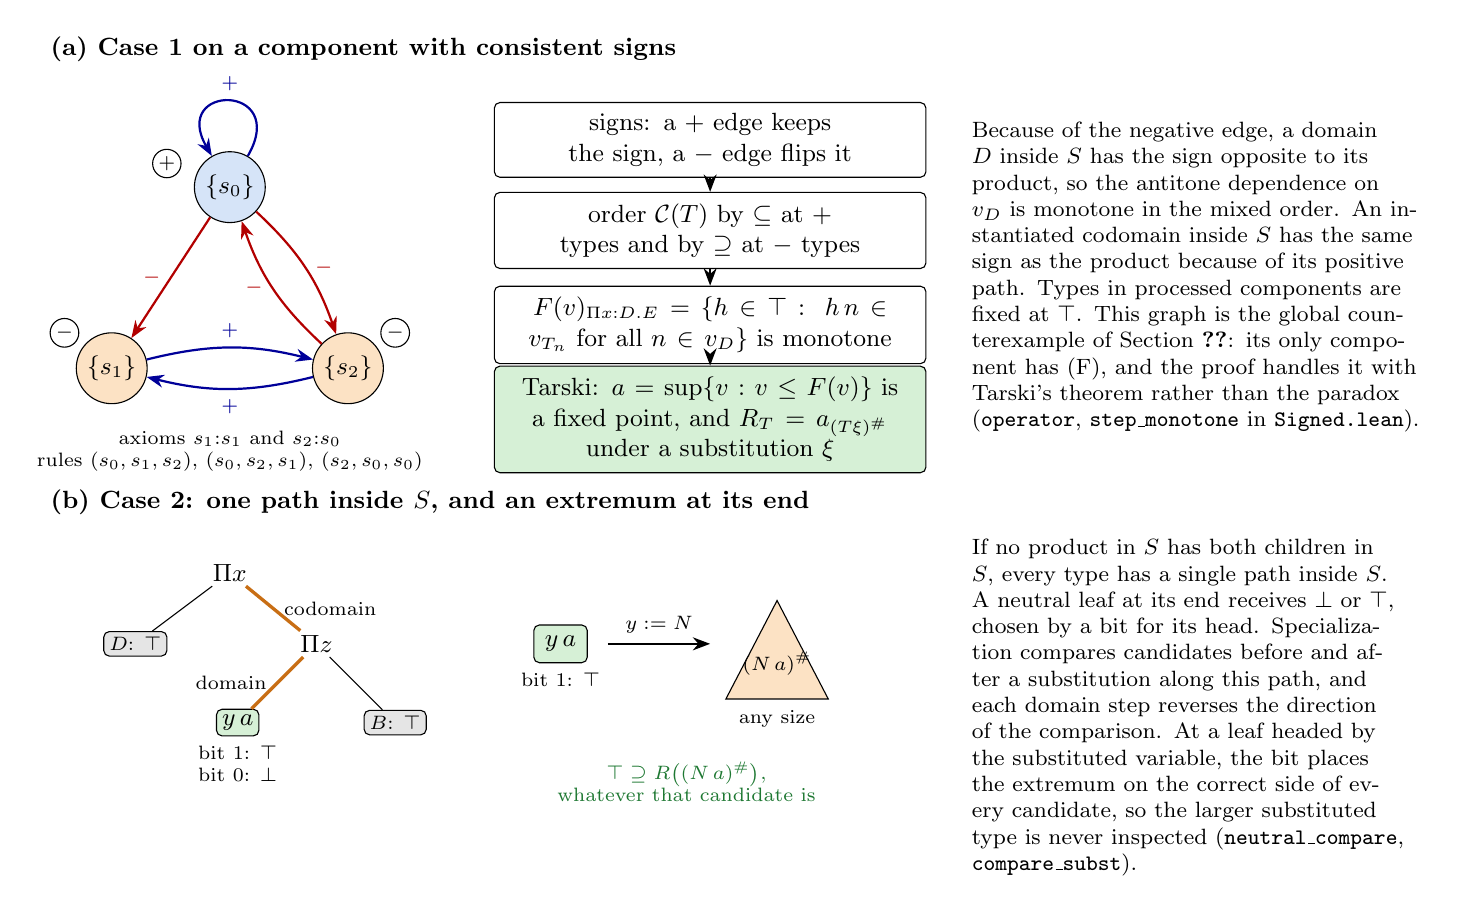
\begin{tikzpicture}[x=1cm,y=1cm]
% (a) Case 1.
\node[font=\small\bfseries,anchor=west] at (-0.6,1.75)
  {(a) Case 1 on a component with consistent signs};
\node[v,fill=cand] (a0) at (1.8,0) {$\{s_0\}$};
\node[v,fill=obs] (a1) at (0.3,-2.3) {$\{s_1\}$};
\node[v,fill=obs] (a2) at (3.3,-2.3) {$\{s_2\}$};
\draw[posedge] (a0) to[out=60,in=120,looseness=6] node[lbl,above] {$+$} (a0);
\draw[negedge] (a0) -- node[lbl,left] {$-$} (a1);
\draw[negedge] (a0) to[bend left=14] node[lbl,right] {$-$} (a2);
\draw[negedge] (a2) to[bend left=14] node[lbl,left] {$-$} (a0);
\draw[posedge] (a1) to[bend left=14] node[lbl,above] {$+$} (a2);
\draw[posedge] (a2) to[bend left=14] node[lbl,below] {$+$} (a1);
\node[signb] at (1.0,0.3) {$+$};
\node[signb] at (-0.3,-1.85) {$-$};
\node[signb] at (3.9,-1.85) {$-$};
\node[lbl,align=center] at (1.8,-3.35)
  {axioms $s_1{:}s_1$ and $s_2{:}s_0$\\ rules $(s_0,s_1,s_2)$, $(s_0,s_2,s_1)$, $(s_2,s_0,s_0)$};
\node[box,text width=5.2cm,fill=white] (m1) at (7.9,0.6)
  {signs: a $+$ edge keeps the sign, a $-$ edge flips it};
\node[box,text width=5.2cm,fill=white] (m2) at (7.9,-0.55)
  {order $\mathcal C(T)$ by $\subseteq$ at $+$ types and by $\supseteq$ at $-$ types};
\node[box,text width=5.2cm,fill=white] (m3) at (7.9,-1.75)
  {$F(v)_{\Pi x:D.E}=\{h\in\top:\ h\,n\in v_{T_n}\text{ for all }n\in v_D\}$
   is monotone};
\node[box,text width=5.2cm,fill=easy] (m4) at (7.9,-2.95)
  {Tarski: $a=\sup\{v: v\le F(v)\}$ is a fixed point, and $R_T=a_{(T\xi)^\#}$
   under a substitution $\xi$};
\draw[arr] (m1) -- (m2); \draw[arr] (m2) -- (m3); \draw[arr] (m3) -- (m4);
\node[expl,text width=5.7cm] at (11.1,0.95)
  {Because of the negative edge, a domain $D$ inside $S$ has the sign opposite to
   its product, so the antitone dependence on $v_D$ is monotone in the mixed order. An
   instantiated codomain inside $S$ has the same sign as the product because of its
   positive path. Types in processed components are fixed at $\top$. This graph is
   the global counterexample of Section~\ref{sec:reduce}: its only component has (F),
   and the proof handles it with Tarski's theorem rather than the paradox
   (\texttt{operator}, \texttt{step\_monotone} in \texttt{Signed.lean}).};
% (b) Case 2.
\begin{scope}[yshift=-5.3cm]
\node[font=\small\bfseries,anchor=west] at (-0.6,1.3)
  {(b) Case 2: one path inside $S$, and an extremum at its end};
\node[tn] (p0) at (1.8,0.4) {$\Pi x$};
\node[box,fill=shared,font=\scriptsize,inner sep=2pt] (pD) at (0.6,-0.5) {$D$: $\top$};
\node[tn] (p1) at (2.9,-0.5) {$\Pi z$};
\node[box,fill=easy,inner sep=2pt] (pL) at (1.9,-1.5) {$y\,a$};
\node[box,fill=shared,font=\scriptsize,inner sep=2pt] (pB) at (3.9,-1.5) {$B$: $\top$};
\draw (p0) -- (pD);
\draw[very thick,pathc] (p0) -- node[lbl,right,text=black] {codomain} (p1);
\draw[very thick,pathc] (p1) -- node[lbl,left,text=black] {domain} (pL);
\draw (p1) -- (pB);
\node[lbl,align=center,anchor=north] at (pL.south) {bit $1$: $\top$\\ bit $0$: $\bot$};
\node[box,fill=easy] (lf) at (6.0,-0.5) {$y\,a$};
\node[lbl,anchor=north] at (lf.south) {bit $1$: $\top$};
\draw[arr] (6.6,-0.5) -- node[lbl,above] {$y:=N$} (7.9,-0.5);
\draw[fill=obs] (8.1,-1.2) -- (8.75,0.05) -- (9.4,-1.2) -- cycle;
\node[lbl] at (8.75,-0.75) {$(N\,a)^\#$};
\node[lbl,anchor=north] at (8.75,-1.22) {any size};
\node[lbl,text=okgreen,align=center] at (7.6,-2.25)
  {$\top\supseteq R\bigl((N\,a)^\#\bigr)$,\\ whatever that candidate is};
\node[expl,text width=5.7cm] at (11.1,0.95)
  {If no product in $S$ has both children in $S$, every type has a single path inside
   $S$. A neutral leaf at its end receives $\bot$ or $\top$, chosen by a bit for its
   head. Specialization compares candidates before and after a substitution along
   this path, and each domain step reverses the direction of the comparison. At a
   leaf headed by the substituted variable, the bit places the extremum on the
   correct side of every candidate, so the larger substituted type is never inspected
   (\texttt{neutral\_compare}, \texttt{compare\_subst}).};
\end{scope}
\end{tikzpicture}
\caption{The two simple constructions. (a)~Blue vertices have sign $+$ and orange ones
sign $-$, and since every closed walk is even, the signs are well defined. (b)~A
schematic type $T=\Pi x{:}D.\,\Pi z{:}(y\,a).\,B$, not taken from a particular
specification, whose path inside $S$ (orange) goes first to the codomain and then to
the domain. Children off the path lie in processed components and receive $\top$.
After one domain step the comparison runs backwards, so the leaf needs $\top$.}
\label{fig:case12}
\end{figure}

\paragraph{Case 3.} When both tests fail, the proof follows Girard: each variable
receives a parameter, and a type is interpreted by evaluating its syntax
(Figure~\ref{fig:case3}). The parameter of a variable $X$ of type $\Pi y{:}A.\,s$
must specify which candidate $X\,a$ denotes for every possible argument $a$, so it is
a table indexed by arguments. Specialization, the law for substituting an argument
into a codomain, is then proved by transporting a typing tree along substitution and
reduction.

\begin{figure}[H]
\centering
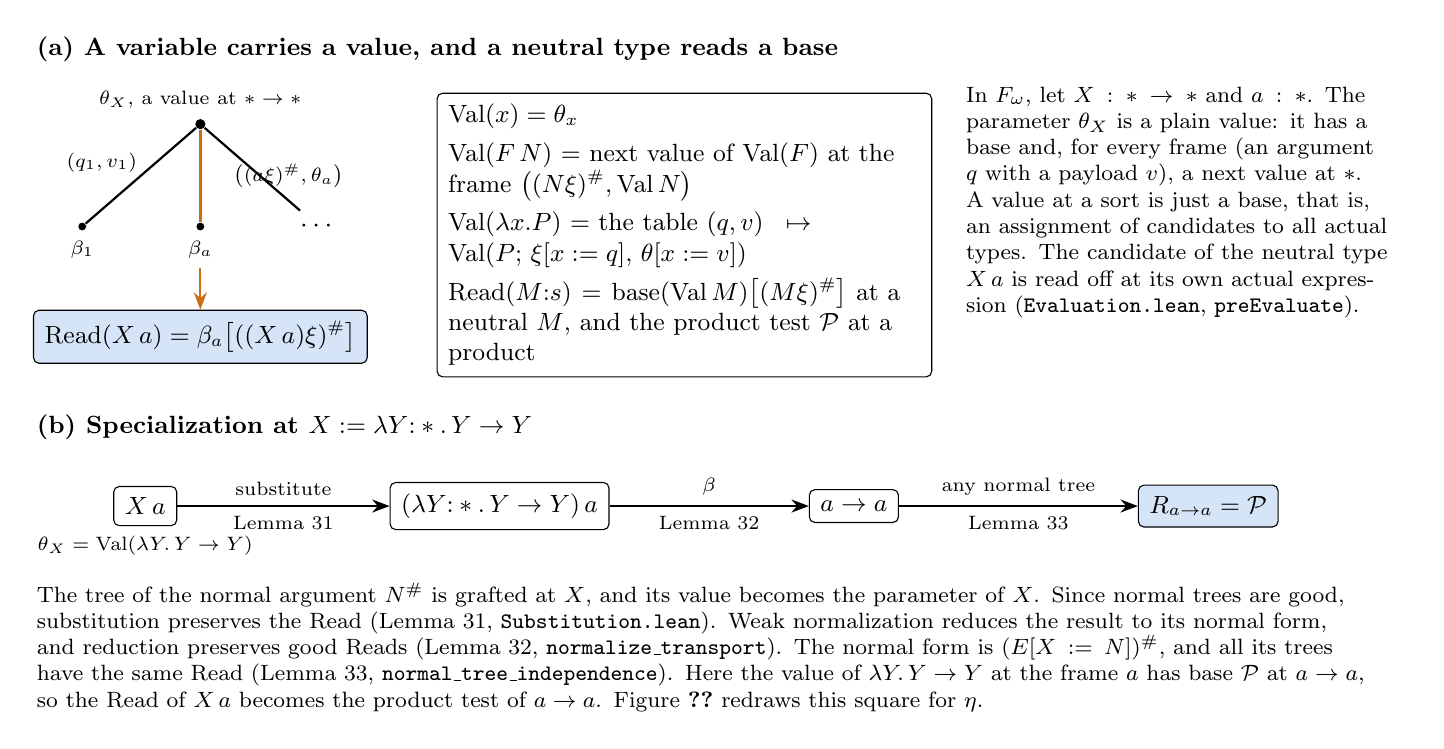
\begin{tikzpicture}[x=1cm,y=1cm]
% (a) Values and Reads.
\node[font=\small\bfseries,anchor=west] at (-0.6,1.3)
  {(a) A variable carries a value, and a neutral type reads a base};
\node[circle,fill=black,inner sep=1.3pt] (r) at (1.6,0.35) {};
\node[lbl,anchor=south] at (r.north) {$\theta_X$, a value at $*\to*$};
\node[circle,fill=black,inner sep=1pt] (v1) at (0.1,-0.95) {};
\node[circle,fill=black,inner sep=1pt] (v2) at (1.6,-0.95) {};
\node (v3) at (3.1,-0.95) {$\cdots$};
\draw[thick] (r) -- node[lbl,above left,inner sep=1pt] {$(q_1,v_1)$} (v1);
\draw[very thick,pathc] (r) -- node[lbl,anchor=west,xshift=8pt,text=black] {$\bigl((a\xi)^\#,\theta_a\bigr)$} (v2);
\draw[thick] (r) -- (v3);
\node[lbl,anchor=north] at (v1.south) {$\beta_1$};
\node[lbl,anchor=north] (ba) at (v2.south) {$\beta_a$};
\node[box,fill=cand] (rd) at (1.6,-2.35) {$\Read(X\,a)=\beta_a\bigl[((X\,a)\xi)^\#\bigr]$};
\draw[arr,pathc] (ba) -- (rd);
\node[box,fill=white,text width=6.0cm,align=left,anchor=north west] at (4.6,0.75)
  {$\Val(x)=\theta_x$\\[3pt]
   $\Val(F\,N)$ = next value of $\Val(F)$ at the frame $\bigl((N\xi)^\#,\Val N\bigr)$\\[3pt]
   $\Val(\lambda x.P)$ = the table $(q,v)\mapsto\Val(P;\,\xi[x:=q],\,\theta[x:=v])$\\[3pt]
   $\Read(M{:}s)=\mathrm{base}(\Val M)\bigl[(M\xi)^\#\bigr]$ at a neutral $M$, and the
   product test $\mathcal P$ at a product};
\node[expl,text width=5.6cm] at (11.2,0.95)
  {In $F_\omega$, let $X:*\to*$ and $a:*$. The parameter $\theta_X$ is a plain value:
   it has a base and, for every frame (an argument $q$ with a payload $v$), a next
   value at $*$. A value at a sort is just a base, that is, an assignment of
   candidates to all actual types. The candidate of the neutral type $X\,a$ is read
   off at its own actual expression (\texttt{Evaluation.lean},
   \texttt{preEvaluate}).};
% (b) Specialization.
\begin{scope}[yshift=-4.5cm]
\node[font=\small\bfseries,anchor=west] at (-0.6,1.0)
  {(b) Specialization at $X:=\lambda Y{:}*.\,Y\to Y$};
\node[box,fill=white] (s1) at (0.9,0) {$X\,a$};
\node[lbl,anchor=north] at (s1.south) {$\theta_X=\Val(\lambda Y.\,Y\to Y)$};
\node[box,fill=white] (s2) at (5.4,0) {$(\lambda Y{:}*.\,Y\to Y)\,a$};
\node[box,fill=white] (s3) at (9.9,0) {$a\to a$};
\node[box,fill=cand] (s4) at (14.4,0) {$R_{a\to a}=\mathcal P$};
\draw[arr] (s1) -- node[lbl,above] {substitute} node[lbl,below] {Lemma 31} (s2);
\draw[arr] (s2) -- node[lbl,above] {$\beta$} node[lbl,below] {Lemma 32} (s3);
\draw[arr] (s3) -- node[lbl,above] {any normal tree} node[lbl,below] {Lemma 33} (s4);
\node[expl,text width=16.9cm] at (-0.6,-0.85)
  {The tree of the normal argument $N^\#$ is grafted at $X$, and its value becomes the
   parameter of $X$. Since normal trees are good, substitution preserves the Read
   (Lemma~31, \texttt{Substitution.lean}). Weak normalization reduces the result to
   its normal form, and reduction preserves good Reads (Lemma~32,
   \texttt{normalize\_transport}). The normal form is $(E[X:=N])^\#$, and all its trees
   have the same Read (Lemma~33, \texttt{normal\_tree\_independence}). Here the value of
   $\lambda Y.\,Y\to Y$ at the frame $a$ has base $\mathcal P$ at $a\to a$, so the Read
   of $X\,a$ becomes the product test of $a\to a$. Figure~\ref{fig:subst} redraws this
   square for $\eta$.};
\end{scope}
\end{tikzpicture}
\caption{Case~3 on the simplest example. (a)~Evaluation assigns values to terms and
candidates to types, and the orange frame is the one used by $X\,a$. (b)~The
specialization law of the interface, proved by three transport lemmas, numbered as
in OpenAI's preprint.}
\label{fig:case3}
\end{figure}

\paragraph{The parameter spaces.} The space of $\theta_X$ depends on the spaces at
the domains and targets of the frames of its type, and these dependencies can form
cycles. The proof builds the spaces in two ways (Figure~\ref{fig:spaces}), and the
forbidden configuration is exactly the case in which neither works.

\begin{figure}[H]
\centering
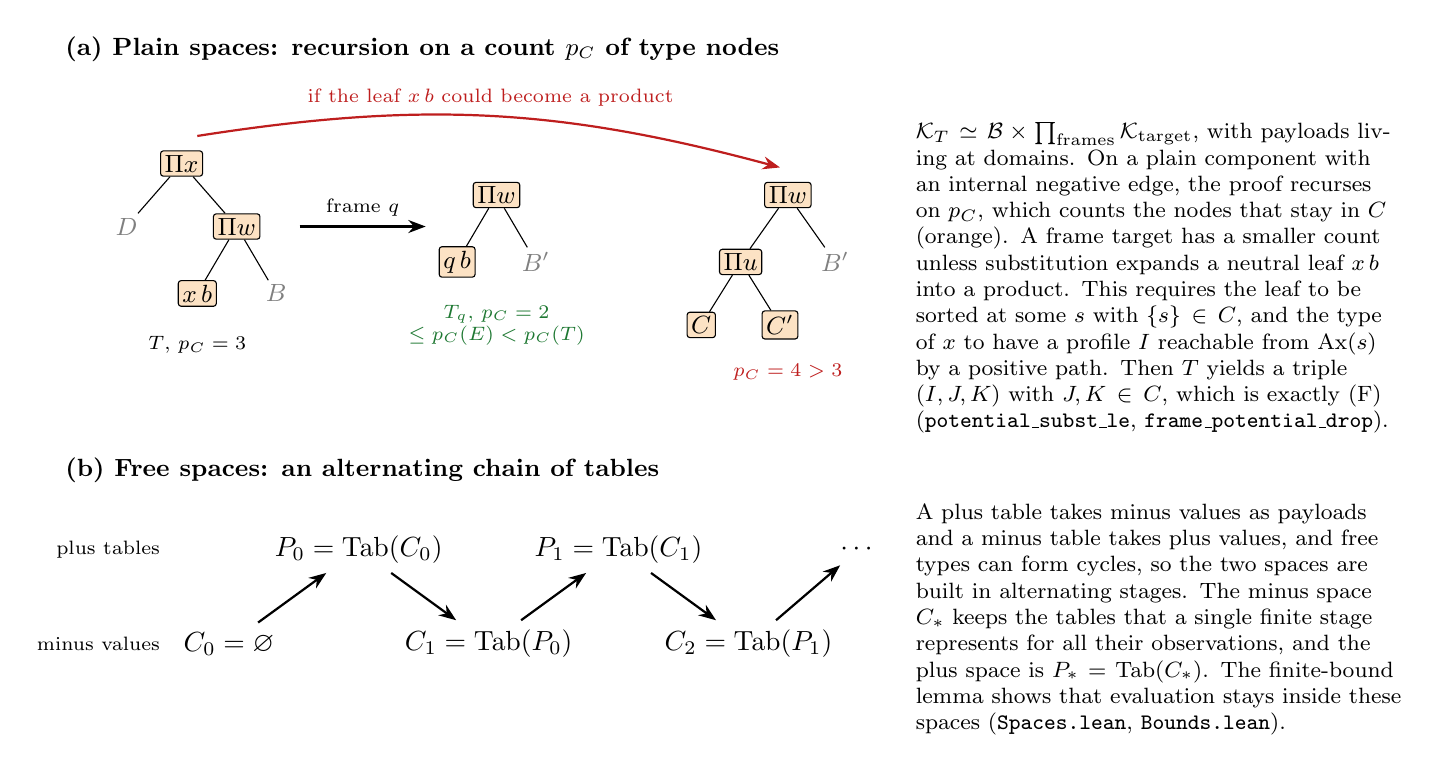
\begin{tikzpicture}[x=1cm,y=1cm]
% (a) Plain spaces and the count.
\node[font=\small\bfseries,anchor=west] at (-0.6,1.75)
  {(a) Plain spaces: recursion on a count $p_C$ of type nodes};
\node[cn] (t0) at (1.0,0.3) {$\Pi x$};
\node[un] (tD) at (0.3,-0.5) {$D$};
\node[cn] (tE) at (1.7,-0.5) {$\Pi w$};
\node[cn] (tL) at (1.2,-1.35) {$x\,b$};
\node[un] (tB) at (2.2,-1.35) {$B$};
\draw (t0) -- (tD); \draw (t0) -- (tE); \draw (tE) -- (tL); \draw (tE) -- (tB);
\node[lbl] at (1.2,-2.0) {$T$, $p_C=3$};
\node[cn] (g0) at (5.0,-0.1) {$\Pi w$};
\node[cn] (gL) at (4.5,-0.95) {$q\,b$};
\node[un] (gB) at (5.5,-0.95) {$B'$};
\draw (g0) -- (gL); \draw (g0) -- (gB);
\node[lbl,text=okgreen,align=center] at (5.0,-1.75) {$T_q$, $p_C=2$\\ $\le p_C(E)<p_C(T)$};
\draw[arr] (2.5,-0.5) -- node[lbl,above] {frame $q$} (4.1,-0.5);
\node[cn] (b0) at (8.7,-0.1) {$\Pi w$};
\node[cn] (bL) at (8.1,-0.95) {$\Pi u$};
\node[cn] (bC) at (7.6,-1.75) {$C$};
\node[cn] (bC2) at (8.6,-1.75) {$C'$};
\node[un] (bB) at (9.3,-0.95) {$B'$};
\draw (b0) -- (bL); \draw (b0) -- (bB); \draw (bL) -- (bC); \draw (bL) -- (bC2);
\node[lbl,text=warn] at (8.7,-2.35) {$p_C=4>3$};
\draw[arr,warn] (1.2,0.65) to[bend left=12] node[lbl,above] {if the leaf $x\,b$ could
  become a product} (8.6,0.25);
\node[expl,text width=6.3cm] at (10.2,0.95)
  {$\mathcal K_T\simeq\mathcal B\times\prod_{\text{frames}}\mathcal K_{\text{target}}$,
   with payloads living at domains. On a plain component with an internal negative
   edge, the proof recurses on $p_C$, which counts the nodes that stay in $C$
   (orange). A frame target has a smaller count unless substitution expands a neutral
   leaf $x\,b$ into a product. This requires the leaf to be sorted at some $s$ with
   $\{s\}\in C$, and the type of $x$ to have a profile $I$ reachable from
   $\operatorname{Ax}(s)$ by a positive path. Then $T$ yields a triple $(I,J,K)$ with
   $J,K\in C$, which is exactly (F) (\texttt{potential\_subst\_le},
   \texttt{frame\_potential\_drop}).};
% (b) Free spaces and the alternating chain.
\begin{scope}[yshift=-4.6cm]
\node[font=\small\bfseries,anchor=west] at (-0.6,1.0)
  {(b) Free spaces: an alternating chain of tables};
\node[lbl,anchor=east] at (0.85,0) {plus tables};
\node[lbl,anchor=east] at (0.85,-1.2) {minus values};
\node (c0) at (1.6,-1.2) {$C_0=\varnothing$};
\node (p0) at (3.25,0) {$P_0=\mathrm{Tab}(C_0)$};
\node (c1) at (4.9,-1.2) {$C_1=\mathrm{Tab}(P_0)$};
\node (p1) at (6.55,0) {$P_1=\mathrm{Tab}(C_1)$};
\node (c2) at (8.2,-1.2) {$C_2=\mathrm{Tab}(P_1)$};
\node (dd) at (9.6,0) {$\cdots$};
\draw[arr] (c0) -- (p0); \draw[arr] (p0) -- (c1); \draw[arr] (c1) -- (p1);
\draw[arr] (p1) -- (c2); \draw[arr] (c2) -- (dd);
\node[expl,text width=6.3cm] at (10.2,0.7)
  {A plus table takes minus values as payloads and a minus table takes plus values,
   and free types can form cycles, so the two spaces are built in alternating stages.
   The minus space $C_*$ keeps the tables that a single finite stage represents for
   all their observations, and the plus space is $P_*=\mathrm{Tab}(C_*)$. The
   finite-bound lemma shows that evaluation stays inside these spaces
   (\texttt{Spaces.lean}, \texttt{Bounds.lean}).};
\end{scope}
\end{tikzpicture}
\caption{The two kinds of parameter spaces in case~3. (a)~Orange nodes are counted by
$p_C$ and gray ones are not. The left arrow is a legal frame, and the red arrow is
the expansion that (F) would permit. The trees are schematic rather than taken from a
particular specification, and the count $4$ only illustrates that an expansion can
raise $p_C$. (b)~A table in $\mathrm{Tab}(Y)$ gives a base observation for every
continuing stack of frames and an exit observation for every exiting stack, and the
opposite-sign payloads in these stacks come from $Y$.}
\label{fig:spaces}
\end{figure}

\clearpage
%======================================================================
\section{The forbidden configuration on familiar systems}\label{sec:forbidden}

The forbidden configuration (F) is the configuration prohibited by condition~(7) in
Section~5 of OpenAI's preprint~\cite{OpenAI2026}. It involves the current component
$S$ and a strongly connected piece $C$ of the \emph{secondary graph}. The vertices of
the secondary graph are the profiles reached by positive paths from the layers
$\Ax(s)$ with $\{s\}\in S$. Its edges are the positive edges between these vertices,
together with the negative edge $I\to K$ of each triple $(I,J,K)$ whose three
profiles are all vertices. A vertex is \emph{direct} if it is the domain $I$ of a
triple $(I,J,K)$ with $J,K\in S$. The configuration requires the following.
\begin{enumerate}[label=(\alph*)]
\item $C$ is plain (it reaches direct vertices along paths of both parities) and
  has an internal negative edge.
\item There is a profile triple $(I,J,K)$ with $J,K\in C$.
\item There is a sort $s$ with $\{s\}\in C$ and $\Ax(s)\neq\emptyset$, so that $C$
  contains \emph{variables} of sort $s$.
\item There is a positive path $\Ax(s)\to I$, so that a product in $C$ can
  \emph{quantify over} the inhabitants of $s$.
\end{enumerate}
Informally, (F) is a layer of types that has variables and can quantify over
itself. Among the systems of Table~\ref{tab:systems}, the configuration occurs
exactly in $\lambda U^-$, $\lambda U$ and $\lambda{*}$, the three systems that are
not normalizing. The sharpest contrast is between $\lambda\mathrm{HOL}$ and
$\lambda U^-$, which differ only by the rule $(\triangle,\square)$. This rule
creates the edge $\{\triangle\}\to\{\square\}$ that completes the configuration.

\begin{figure}[H]
\centering
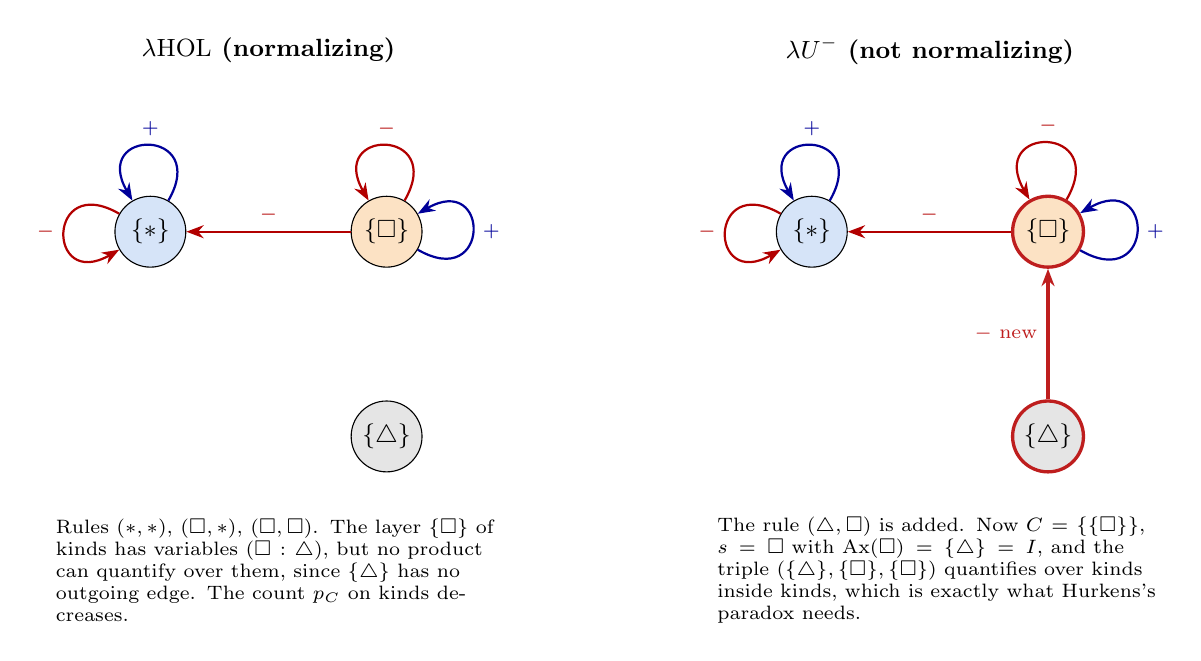
\begin{tikzpicture}[x=1cm,y=1cm]
\begin{scope}
\node[font=\small\bfseries] at (1.5,2.3) {$\lambda\mathrm{HOL}$ (normalizing)};
\node[v,fill=cand] (s) at (0,0) {$\{*\}$};
\node[v,fill=obs] (b) at (3,0) {$\{\square\}$};
\node[v,fill=shared] (t) at (3,-2.6) {$\{\triangle\}$};
\draw[negedge] (s) to[out=150,in=210,looseness=6] node[left,font=\scriptsize] {$-$} (s);
\draw[posedge] (s) to[out=60,in=120,looseness=6] node[above,font=\scriptsize] {$+$} (s);
\draw[negedge] (b) to[out=60,in=120,looseness=6] node[above,font=\scriptsize] {$-$} (b);
\draw[posedge] (b) to[out=-30,in=30,looseness=6] node[right,font=\scriptsize] {$+$} (b);
\draw[negedge] (b) -- node[above,font=\scriptsize] {$-$} (s);
\node[font=\scriptsize,text width=5.6cm,align=left] at (1.6,-4.3)
  {Rules $(*,*)$, $(\square,*)$, $(\square,\square)$. The layer $\{\square\}$ of kinds has
   variables ($\square:\triangle$), but no product can quantify over them, since
   $\{\triangle\}$ has no outgoing edge. The count $p_C$ on kinds decreases.};
\end{scope}
\begin{scope}[xshift=8.4cm]
\node[font=\small\bfseries] at (1.5,2.3) {$\lambda U^-$ (not normalizing)};
\node[v,fill=cand] (s) at (0,0) {$\{*\}$};
\node[v,fill=obs,very thick,draw=warn] (b) at (3,0) {$\{\square\}$};
\node[v,fill=shared,very thick,draw=warn] (t) at (3,-2.6) {$\{\triangle\}$};
\draw[negedge] (s) to[out=150,in=210,looseness=6] node[left,font=\scriptsize] {$-$} (s);
\draw[posedge] (s) to[out=60,in=120,looseness=6] node[above,font=\scriptsize] {$+$} (s);
\draw[negedge] (b) to[out=60,in=120,looseness=6] node[above,font=\scriptsize] {$-$} (b);
\draw[posedge] (b) to[out=-30,in=30,looseness=6] node[right,font=\scriptsize] {$+$} (b);
\draw[negedge] (b) -- node[above,font=\scriptsize] {$-$} (s);
\draw[negedge,very thick,warn] (t) -- node[left,font=\scriptsize,text=warn] {$-$ new} (b);
\node[font=\scriptsize,text width=5.6cm,align=left] at (1.6,-4.3)
  {The rule $(\triangle,\square)$ is added. Now $C=\{\{\square\}\}$, $s=\square$ with
   $\Ax(\square)=\{\triangle\}=I$, and the triple
   $(\{\triangle\},\{\square\},\{\square\})$ quantifies over kinds inside kinds,
   which is exactly what Hurkens's paradox needs.};
\end{scope}
\end{tikzpicture}
\caption{Primary graphs of $\lambda\mathrm{HOL}$ and $\lambda U^-$. Red arrows are
domain edges ($-$) and blue arrows codomain edges ($+$). For the component
$S=\{\{*\}\}$, the secondary graph consists of the single vertex
$\{\square\}=\Ax(*)$ with its negative loop, so in both systems $\{\square\}$ is
plain with an internal negative edge. Conditions (c) and (d) hold only in
$\lambda U^-$.}
\label{fig:systems}
\end{figure}

\begin{table}[H]
\centering\small
\begin{tabular}{lll}
\toprule
system & components and constructions used & paradox needed\\
\midrule
$\lambda{\to}$ & $\{\square\}$ case 1, $\{*\}$ case 3 without parameters & no\\
$\lambda 2$ (System F) & $\{\square\}$ case 1, $\{*\}$ case 3 with a free plus layer $\{\square\}$ & no\\
$\lambda P$ (LF) & $\{\square\}$ case 1, $\{*\}$ case 3 without parameters & no\\
$\lambda\omega$ ($F_\omega$) & $\{\square\}$ case 3 without parameters, $\{*\}$ case 3 with a plain layer (count) & no\\
$\lambda C$ (CC) & $\{*,\square\}$ case 3 with a plain layer (count) & no\\
$\lambda\mathrm{HOL}$ & $\{\triangle\}$ case 1, $\{\square\}$ case 3, $\{*\}$ case 3 with a plain layer (count) & no\\
$\lambda U^-$, $\lambda U$ & as $\lambda\mathrm{HOL}$, plus a free plus layer, and (F) at $\{*\}$ & yes\\
$\lambda{*}$ & $\{*\}$ case 3, plain layer, (F) at $\{*\}$ & yes\\
\bottomrule
\end{tabular}
\caption{Components of the standard systems and the constructions that handle them,
computed from the definitions in \texttt{Profiles.lean}. A free or plain layer is a
vertex of the secondary graph whose parameter space is built by case~3. No system in
the table uses case~2 or a free minus layer, so none of them exercises the uniform
stage bounds of \texttt{Bounds.lean}.}
\label{tab:systems}
\end{table}

\paragraph{How the paradox excludes (F).} Figure~\ref{fig:paradox} presents the
paradox half as a sequence of steps. Steps~1 to~6 build, inside the given PTS, a
proof of a terminal formula from the forbidden configuration, and steps~7 and~8 turn
weak normalization into a contradiction. Only step~7 uses the hypothesis.

\begin{figure}[H]
\centering
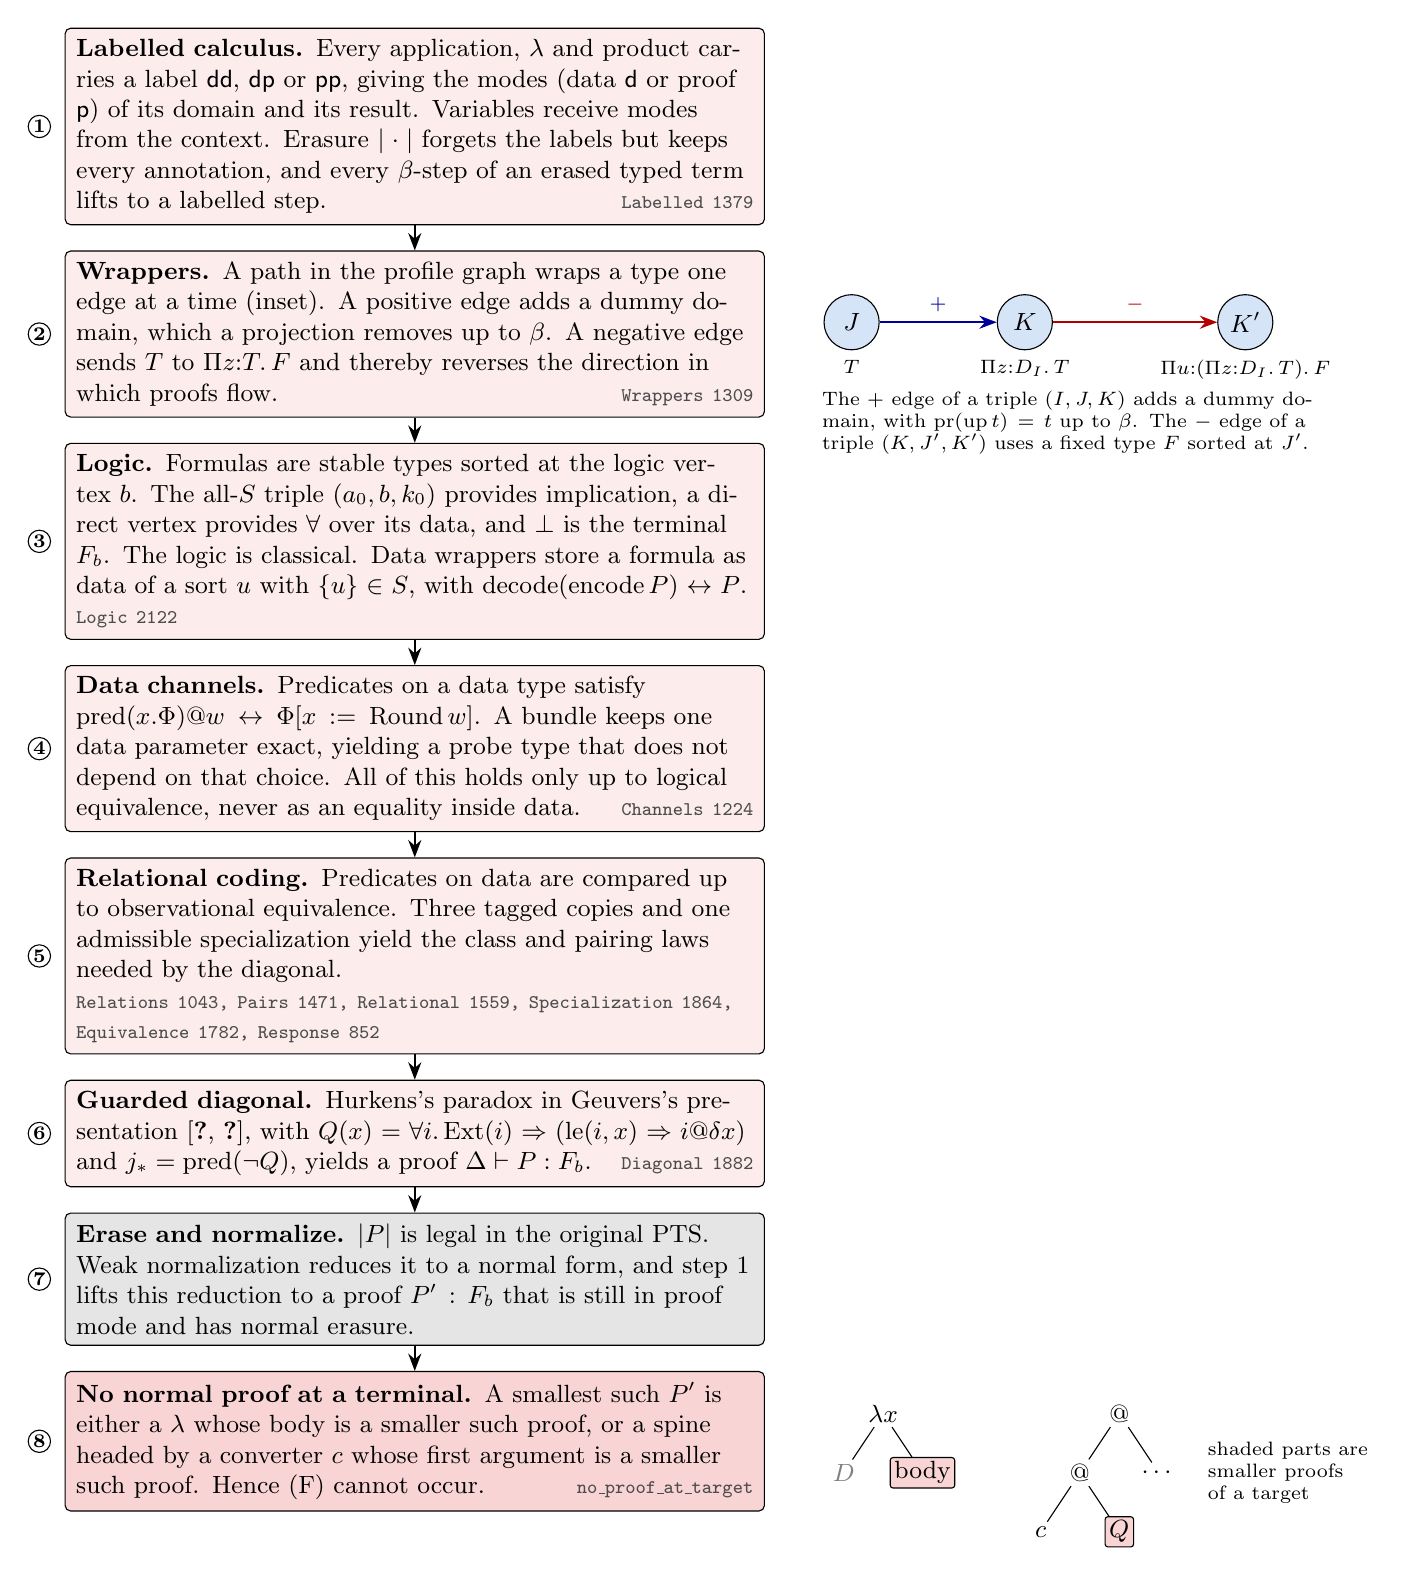
\begin{tikzpicture}[node distance=3.2mm,box/.append style={align=left}]
\node[box,fill=par!45,text width=8.6cm] (b1) at (0,0)
  {\textbf{Labelled calculus.} Every application, $\lambda$ and product carries a
   label $\mathsf{dd}$, $\mathsf{dp}$ or $\mathsf{pp}$, giving the modes (data
   $\mathsf d$ or proof $\mathsf p$) of its domain and its result. Variables receive
   modes from the context. Erasure $|\cdot|$ forgets the labels but keeps every
   annotation, and every $\beta$-step of an erased typed term lifts to a labelled
   step. \hfill{\lean Labelled 1379}};
\node[box,fill=par!45,text width=8.6cm,below=of b1] (b2)
  {\textbf{Wrappers.} A path in the profile graph wraps a type one edge at a time
   (inset). A positive edge adds a dummy domain, which a projection removes up to
   $\beta$. A negative edge sends $T$ to $\Pi z{:}T.\,F$ and thereby reverses the
   direction in which proofs flow. \hfill{\lean Wrappers 1309}};
\node[box,fill=par!45,text width=8.6cm,below=of b2] (b3)
  {\textbf{Logic.} Formulas are stable types sorted at the logic vertex $b$. The
   all-$S$ triple $(a_0,b,k_0)$ provides implication, a direct vertex provides
   $\forall$ over its data, and $\bot$ is the terminal $F_b$. The logic is classical.
   Data wrappers store a formula as data of a sort $u$ with $\{u\}\in S$, with
   $\mathrm{decode}(\mathrm{encode}\,P)\leftrightarrow P$.
   \hfill\mbox{\lean Logic 2122}};
\node[box,fill=par!45,text width=8.6cm,below=of b3] (b4)
  {\textbf{Data channels.} Predicates on a data type satisfy
   $\mathrm{pred}(x.\Phi)@w\leftrightarrow\Phi[x:=\mathrm{Round}\,w]$. A bundle keeps
   one data parameter exact, yielding a probe type that does not depend on that
   choice. All of this holds only up to logical equivalence, never as an equality
   inside data. \hfill\mbox{\lean Channels 1224}};
\node[box,fill=par!45,text width=8.6cm,below=of b4] (b5)
  {\textbf{Relational coding.} Predicates on data are compared up to observational
   equivalence. Three tagged copies and one admissible specialization yield the class
   and pairing laws needed by the diagonal.\\
   {\lean Relations 1043, Pairs 1471, Relational 1559, Specialization 1864,
   Equivalence 1782, Response 852}};
\node[box,fill=par!45,text width=8.6cm,below=of b5] (b6)
  {\textbf{Guarded diagonal.} Hurkens's paradox in Geuvers's
   presentation~\cite{Hurkens1995,Geuvers2007}, with
   $Q(x)=\forall i.\,\mathrm{Ext}(i)\Rightarrow(\mathrm{le}(i,x)\Rightarrow
   i@\delta x)$ and $j_*=\mathrm{pred}(\neg Q)$, yields a proof
   $\Delta\vdash P:F_b$. \hfill{\lean Diagonal 1882}};
\node[box,fill=shared,text width=8.6cm,below=of b6] (b7)
  {\textbf{Erase and normalize.} $|P|$ is legal in the original PTS. Weak
   normalization reduces it to a normal form, and step~1 lifts this reduction to a
   proof $P':F_b$ that is still in proof mode and has normal erasure.};
\node[box,fill=par,text width=8.6cm,below=of b7] (b8)
  {\textbf{No normal proof at a terminal.} A smallest such $P'$ is either a
   $\lambda$ whose body is a smaller such proof, or a spine headed by a converter $c$
   whose first argument is a smaller such proof. Hence (F) cannot occur.
   \hfill{\lean no\_proof\_at\_target}};
\foreach \i in {1,...,8} \node[stepc] at ($(b\i.west)+(-0.32,0)$) {\i};
\foreach \a/\b in {b1/b2,b2/b3,b3/b4,b4/b5,b5/b6,b6/b7,b7/b8} \draw[arr] (\a) -- (\b);
% Inset for step 2: wrapping a type along a path with a positive and a negative edge.
\begin{scope}[shift={($(b2.east)+(0.7,0.15)$)}]
\node[v,fill=cand,minimum size=7mm] (w0) at (0.4,0) {$J$};
\node[v,fill=cand,minimum size=7mm] (w1) at (2.6,0) {$K$};
\node[v,fill=cand,minimum size=7mm] (w2) at (5.4,0) {$K'$};
\draw[posedge] (w0) -- node[lbl,above] {$+$} (w1);
\draw[negedge] (w1) -- node[lbl,above] {$-$} (w2);
\node[lbl,anchor=north] at (w0.south) {$T$};
\node[lbl,anchor=north] at (w1.south) {$\Pi z{:}D_I.\,T$};
\node[lbl,anchor=north] at (w2.south) {$\Pi u{:}(\Pi z{:}D_I.\,T).\,F$};
\node[lbl,align=left,anchor=north west,text width=6.4cm] at (-0.1,-0.75)
  {The $+$ edge of a triple $(I,J,K)$ adds a dummy domain, with
   $\mathrm{pr}(\mathrm{up}\,t)=t$ up to $\beta$. The $-$ edge of a triple
   $(K,J',K')$ uses a fixed type $F$ sorted at $J'$.};
\end{scope}
% Inset for step 8: the two shapes of a smallest normal proof.
\begin{scope}[shift={($(b8.east)+(0.9,0.35)$)}]
\node[tn] (q0) at (0.6,0) {$\lambda x$};
\node[un] (qD) at (0.1,-0.75) {$D$};
\node[tn,draw,fill=par,rounded corners=1pt] (qb) at (1.1,-0.75) {body};
\draw (q0) -- (qD); \draw (q0) -- (qb);
\node[tn] (s0) at (3.6,0) {$@$};
\node[tn] (s1) at (3.1,-0.75) {$@$};
\node[tn] (s2) at (4.1,-0.75) {$\cdots$};
\node[tn] (sc) at (2.6,-1.5) {$c$};
\node[tn,draw,fill=par,rounded corners=1pt] (sQ) at (3.6,-1.5) {$Q$};
\draw (s0) -- (s1); \draw (s0) -- (s2); \draw (s1) -- (sc); \draw (s1) -- (sQ);
\node[lbl,align=left,anchor=west] at (4.6,-0.75) {shaded parts are\\ smaller proofs\\ of a target};
\end{scope}
\end{tikzpicture}
\caption{The paradox half, step by step. Steps~1 to~6 build a proof of the terminal
formula $F_b$ from the forbidden configuration in a single finite labelled context,
and steps~7 and~8 turn weak normalization into a contradiction. In Lean the chain
consists of \texttt{LogicSetup.exists\_setup}, \texttt{ChannelSetup.exists\_setup\_return},
\texttt{relational\_bottom} and \texttt{no\_proof\_at\_target}, assembled in
\texttt{relational\_exclusion}.}
\label{fig:paradox}
\end{figure}

\clearpage
%======================================================================
\section{A shorter proof?}\label{sec:reduce}

The candidate half consists of three constructions, and the paradox accounts for
more than half of OpenAI's Lean code (Figure~\ref{fig:sizes}). This section asks
which parts are necessary and where a shorter proof might come from. Every notion
used here can be computed on finite graphs from the definitions in
\texttt{Profiles.lean}: feasible profiles, the primary graph, components, the
secondary graph, plain and free layers, and the forbidden configuration. The two
counterexamples below can be verified by hand from these definitions, and the
frequencies are counts over random specifications with two to five sorts.

\begin{figure}[H]
\centering
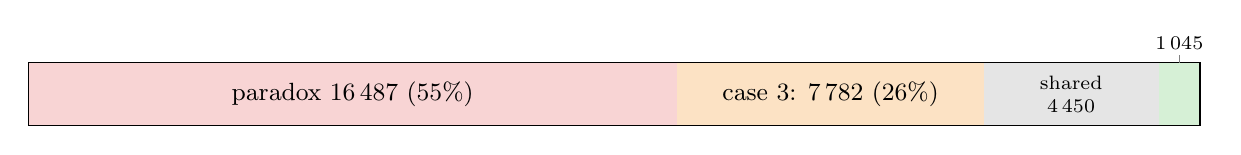
\begin{tikzpicture}[x=0.5mm,y=1cm]
% One unit is 100 lines. The whole bar is 29 764 lines.
\fill[par] (0,0) rectangle (164.87,0.8);
\fill[obs] (164.87,0) rectangle (242.69,0.8);
\fill[shared] (242.69,0) rectangle (287.19,0.8);
\fill[easy] (287.19,0) rectangle (297.64,0.8);
\draw (0,0) rectangle (297.64,0.8);
\node[font=\small] at (82.4,0.4) {paradox 16\,487 (55\%)};
\node[font=\small] at (203.8,0.4) {case 3: 7\,782 (26\%)};
\node[font=\scriptsize,align=center] at (264.9,0.4) {shared\\4\,450};
\node[font=\scriptsize] at (292.4,1.05) {1\,045};
\draw[gray] (292.4,0.8) -- (292.4,0.9);
\end{tikzpicture}
\caption{Lean lines of OpenAI's proof, by part. Cases 1 and 2 form the thin green
slice on the right.}
\label{fig:sizes}
\end{figure}

\paragraph{Cases 1 and 2 cannot be merged into case 3.}
Case~3 needs only the absence of the forbidden configuration (F) at the current
component. If (F) at a component always forced an odd closed walk and an internal
triple there, the paradox would exclude (F) everywhere and cases~1 and~2 could be
deleted. Two specifications show that this fails, in two forms.
\begin{itemize}
\item \emph{Local form.} Take sorts $s_0,s_1,s_2$ with axioms $s_1{:}s_1$,
  $s_2{:}s_1$ and rules $(s_0,s_1,s_2)$, $(s_1,s_0,s_1)$, $(s_1,s_1,s_0)$,
  $(s_1,s_2,s_2)$. The component $\{\{s_2\}\}$ has no odd closed walk but has (F).
\item \emph{Global form}, in which (F) at some case-1 or case-2 component would at
  least imply (F) at some case-3 component. Take axioms $s_1{:}s_1$, $s_2{:}s_0$ and
  rules $(s_0,s_1,s_2)$, $(s_0,s_2,s_1)$, $(s_2,s_0,s_0)$. The only component
  $\{\{s_0\},\{s_1\},\{s_2\}\}$ has no odd closed walk but has (F). There is no
  case-3 component to host the paradox, and the proof handles this system with
  Tarski's theorem alone. Figure~\ref{fig:case12}(a) shows this graph.
\end{itemize}

\begin{figure}[H]
\centering
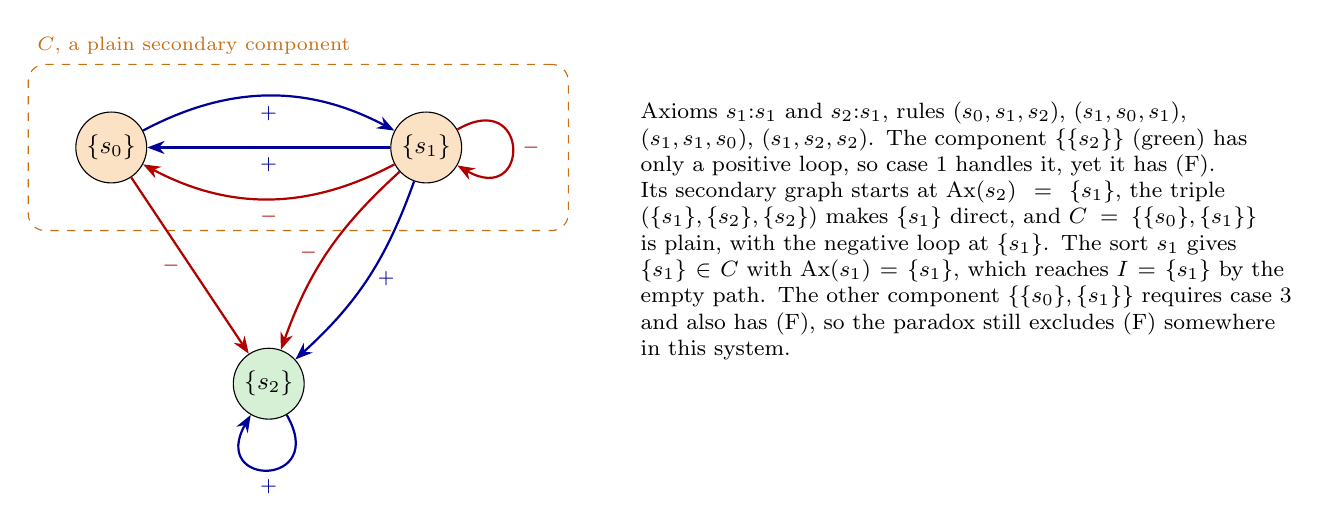
\begin{tikzpicture}[x=1cm,y=1cm]
\node[v,fill=obs] (u0) at (0,0) {$\{s_0\}$};
\node[v,fill=obs] (u1) at (4.0,0) {$\{s_1\}$};
\node[v,fill=easy] (u2) at (2.0,-3.0) {$\{s_2\}$};
\draw[posedge] (u0) to[bend left=28] node[lbl,below] {$+$} (u1);
\draw[posedge] (u1) -- node[lbl,below] {$+$} (u0);
\draw[negedge] (u1) to[bend left=28] node[lbl,below] {$-$} (u0);
\draw[negedge] (u1) to[out=30,in=-30,looseness=6] node[lbl,right] {$-$} (u1);
\draw[posedge] (u1) to[bend left=14] node[lbl,right] {$+$} (u2);
\draw[negedge] (u1) to[bend right=14] node[lbl,left] {$-$} (u2);
\draw[negedge] (u0) -- node[lbl,left] {$-$} (u2);
\draw[posedge] (u2) to[out=-60,in=-120,looseness=6] node[lbl,below] {$+$} (u2);
\begin{scope}[on background layer]
\coordinate (u1r) at ($(u1.east)+(0.75,0)$);
\node[fit=(u0)(u1)(u1r),draw=pathc,dashed,rounded corners=6pt,inner sep=17pt] (cC) {};
\end{scope}
\node[lbl,text=pathc,anchor=south west] at (cC.north west) {$C$, a plain secondary component};
\node[expl,text width=8.4cm] at (6.6,0.7)
  {Axioms $s_1{:}s_1$ and $s_2{:}s_1$, rules $(s_0,s_1,s_2)$, $(s_1,s_0,s_1)$,
   $(s_1,s_1,s_0)$, $(s_1,s_2,s_2)$. The component $\{\{s_2\}\}$ (green) has only a
   positive loop, so case~1 handles it, yet it has (F). Its secondary graph starts at
   $\operatorname{Ax}(s_2)=\{s_1\}$, the triple $(\{s_1\},\{s_2\},\{s_2\})$ makes
   $\{s_1\}$ direct, and $C=\{\{s_0\},\{s_1\}\}$ is plain, with the negative loop at
   $\{s_1\}$. The sort $s_1$ gives $\{s_1\}\in C$ with $\operatorname{Ax}(s_1)
   =\{s_1\}$, which reaches $I=\{s_1\}$ by the empty path. The other component
   $\{\{s_0\},\{s_1\}\}$ requires case~3 and also has (F), so the paradox still
   excludes (F) somewhere in this system.};
\end{tikzpicture}
\caption{The local counterexample: a component can have (F) without an odd closed
walk. In this system a case-3 component has (F) as well, whereas the global
counterexample of Figure~\ref{fig:case12}(a) has no such component.}
\label{fig:local}
\end{figure}
The three constructions therefore complement each other. Since they make up only
3.5\% of the code, this matters more for understanding the proof than for its
length.

\paragraph{Free minus layers are rare.} Free minus layers occur in none of the
standard systems (Table~\ref{tab:systems}), in 1 of 20\,000 random 3-sort
specifications, and in 6 of 28\,000 random functional specifications with 4 or 5
sorts. They therefore do not require non-functional rules, only unusual ones.
Without minus layers a plus table has no opposite-sign payloads, so the alternating
chain is unnecessary, and we expect the same of the uniform bounds.

\paragraph{Many forbidden configurations are not shaped like $\lambda U^-$.} The
paradox needs a way to quantify over a layer of types inside that same layer,
together with a logic in $S$. Rocq's \texttt{Logic/Hurkens.v}~\cite{RocqHurkens}
proves the paradox for an abstract system with two universes in its module
\texttt{Generic}, in about 180 lines with a 60-line core. It needs no reduction rule
at all for the small (formula) universe, but exact $\beta$ for three things at the
large (data) universe: products over data that return to the data sort,
quantification over all data types that returns to it, and a sort of formulas inside
the data universe. We call a configuration \emph{tight} if it contains such a core,
with data-level products that return to the data sort along positive edges, where
OpenAI's wrappers cancel up to $\beta$. Among random specifications that need the
paradox, the counts are as follows.
\begin{itemize}
\item Tight cores exist in about 60\% of these specifications with 2 sorts and in
  about 40\% of those with 3 or 4 sorts. In the remaining ones at least one of the
  three data-level requirements fails, and the failures are spread over all three
  requirements with no dominant one.
\item The return path from the quantified product $K$ to the data layer $\{s\}$ is
  positive in 99.6\% of the configurations (6\,959 of 6\,989), so OpenAI's wrappers
  would cancel up to $\beta$ there. This does not hold in general: the axioms
  $s_0{:}s_0$, $s_0{:}s_1$, $s_0{:}s_2$, $s_1{:}s_0$ with the rules $(s_0,s_2,s_2)$,
  $(s_1,s_2,s_2)$, $(s_2,s_0,s_2)$, $(s_2,s_1,s_0)$, $(s_2,s_2,s_2)$ give (F) but no
  positive return path.
\end{itemize}
OpenAI's general encoding, with its relational coding up to logical equivalence, is
therefore needed. The generic paradox could serve as a fast path for about half of
the configurations, but it would add a second route rather than remove the
relational layer. The open question for a substantially shorter paradox is whether
predicates over data, which OpenAI builds as wrappers into terminal types, can be
given exact $\beta$ in every configuration. Since such a statement is a lemma about
finite graphs, it can be tested on many specifications before any work in Lean.
Table~\ref{tab:assessment} summarizes the section.

\begin{table}[H]
\centering\small
\begin{tabular}{>{\raggedright\arraybackslash}p{3.2cm}>{\raggedright\arraybackslash}p{11.8cm}}
\toprule
part & assessment\\
\midrule
cases 1 and 2 & Needed: the two counterexamples above show that case~3 cannot take
  them over.\\ \addlinespace
free minus layers & Needed in general, but never by the standard systems. A first
  version of the proof for specifications without minus layers could skip the
  uniform bounds (most of \texttt{Bounds.lean}, 1\,142 lines, and the minus half of
  \texttt{Spaces.lean}). Whether a finite specification has free minus layers is
  decided by a finite graph computation.\\ \addlinespace
paradox, generic part & The relational coding (\texttt{Relations}, \texttt{Pairs},
  \texttt{Relational}, \texttt{Specialization}, \texttt{Equivalence},
  \texttt{Response}, about 8\,600 lines) exists because data-level $\beta$ holds
  only up to $\leftrightarrow$ along negative wrappers. For tight configurations,
  Rocq's generic Hurkens paradox (about 180 lines) should apply with exact $\beta$.
  This covers roughly half of the random cases, so it would be a second route rather
  than a replacement.\\ \addlinespace
paradox, encoding part & \texttt{Labelled}, \texttt{Wrappers}, \texttt{Logic} and
  \texttt{Channels} (about 6\,000 lines) build a logic out of an arbitrary profile
  graph. A smarter choice of paths could shorten this part, for instance by proving
  that every configuration contains a smaller one with fewer negative edges on its
  return paths.\\
\bottomrule
\end{tabular}
\caption{Assessment of each part. The first row is settled by the two
counterexamples. The second rests on counts over specifications, and its saving is
expected but has not been checked in Lean. The last two rows are directions, not
results.}
\label{tab:assessment}
\end{table}

\clearpage
%======================================================================
\section{The \texorpdfstring{$\beta\eta$}{beta-eta} proof}\label{sec:be}

The development \texttt{PTS-beta-eta}~\cite{PTSbetaetaLean} proves the same
implication for Geuvers's systems $\mathrm{PTS}_{\beta\eta}$~\cite{Geuvers1993},
whose conversion rule uses $\beta\eta$-conversion: if every legal term is weakly
$\beta\eta$- or weakly $\beta$-normalizing, then every legal term is strongly
$\beta\eta$-normalizing. OpenAI's theorem does not imply this, because
$\mathrm{PTS}_{\beta\eta}$ can type more terms than $\mathrm{PTS}_\beta$, so the
proof reruns OpenAI's argument inside $\mathrm{PTS}_{\beta\eta}$
(Figure~\ref{fig:map-be}). The recursion over components is unchanged, and the new
material comes before it, after it and inside case~3. Notation is explained below
the figure.

\begin{figure}[H]
\centering
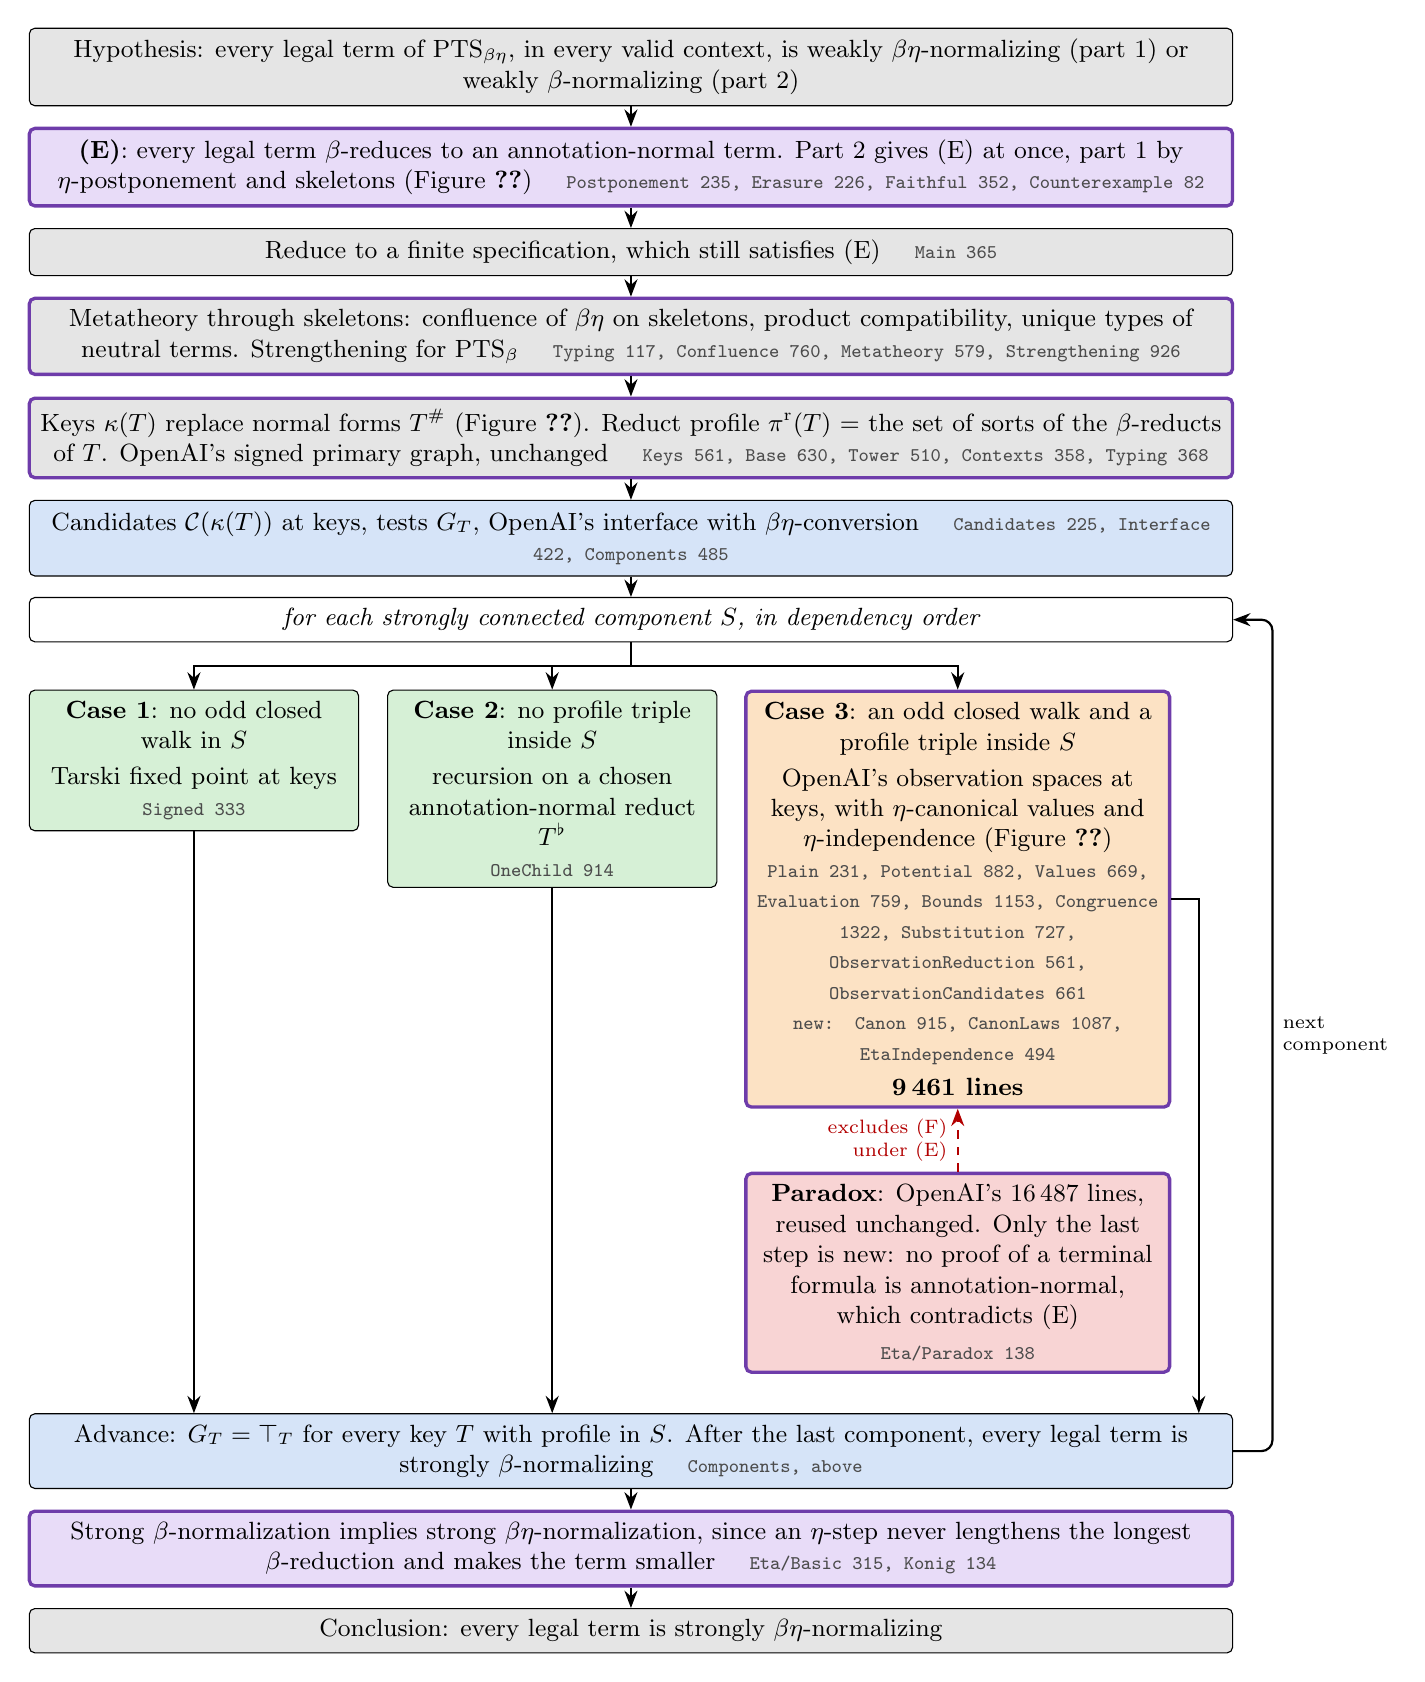
\begin{tikzpicture}[node distance=2.6mm,box/.append style={align=flush center}]
\node[box,fill=shared,text width=15cm] (wn)
  {Hypothesis: every legal term of $\mathrm{PTS}_{\beta\eta}$, in every valid context,
   is weakly $\beta\eta$-normalizing (part~1) or weakly $\beta$-normalizing (part~2)};
\node[newbox,fill=etanew,text width=15cm,below=of wn] (E)
  {\textbf{(E)}: every legal term $\beta$-reduces to an annotation-normal term.
   Part~2 gives (E) at once, part~1 by $\eta$-postponement and skeletons
   (Figure~\ref{fig:E}) \quad
   {\lean Postponement 235, Erasure 226, Faithful 352, Counterexample 82}};
\node[box,fill=shared,text width=15cm,below=of E] (fin)
  {Reduce to a finite specification, which still satisfies (E) \quad {\lean Main 365}};
\node[newbox,fill=shared,text width=15cm,below=of fin] (meta)
  {Metatheory through skeletons: confluence of $\beta\eta$ on skeletons, product
   compatibility, unique types of neutral terms. Strengthening for
   $\mathrm{PTS}_\beta$ \quad
   {\lean Typing 117, Confluence 760, Metatheory 579, Strengthening 926}};
\node[newbox,fill=shared,text width=15cm,below=of meta] (prof)
  {Keys $\kappa(T)$ replace normal forms $T^\#$ (Figure~\ref{fig:keys}). Reduct profile
   $\pi^{\mathrm r}(T)$ = the set of sorts of the $\beta$-reducts of $T$. OpenAI's signed
   primary graph, unchanged \quad
   {\lean Keys 561, Base 630, Tower 510, Contexts 358, Typing 368}};
\node[box,fill=cand,text width=15cm,below=of prof] (cand)
  {Candidates $\mathcal C(\kappa(T))$ at keys, tests $G_T$, OpenAI's interface with
   $\beta\eta$-conversion \quad {\lean Candidates 225, Interface 422, Components 485}};
\node[box,fill=white,text width=15cm,below=of cand,font=\small\itshape] (loop)
  {for each strongly connected component $S$, in dependency order};
\coordinate (row) at ($(loop.south)+(0,-6mm)$);
\node[box,fill=easy,text width=3.9cm,anchor=north] (c1) at (row -| -5.55,0)
  {\textbf{Case 1}: no odd closed walk in $S$\\[2pt]
   Tarski fixed point at keys\\ {\lean Signed 333}};
\node[box,fill=easy,text width=3.9cm,anchor=north] (c2) at (row -| -1.00,0)
  {\textbf{Case 2}: no profile triple inside $S$\\[2pt]
   recursion on a chosen annotation-normal reduct $T^\flat$\\ {\lean OneChild 914}};
\node[newbox,fill=obs,text width=5.1cm,anchor=north] (c3) at (row -| 4.15,0)
  {\textbf{Case 3}: an odd closed walk and a profile triple inside $S$\\[2pt]
   OpenAI's observation spaces at keys, with $\eta$-canonical values and
   $\eta$-independence (Figure~\ref{fig:canon})\\
   {\lean Plain 231, Potential 882, Values 669, Evaluation 759, Bounds 1153,
   Congruence 1322, Substitution 727, ObservationReduction 561,
   ObservationCandidates 661}\\
   {\lean new: Canon 915, CanonLaws 1087, EtaIndependence 494}\\[2pt]
   \textbf{9\,461 lines}};
\node[newbox,fill=par,text width=5.1cm,below=8mm of c3] (par)
  {\textbf{Paradox}: OpenAI's 16\,487 lines, reused unchanged. Only the last step is
   new: no proof of a terminal formula is annotation-normal, which contradicts
   (E)\\[2pt]
   {\lean Eta/Paradox 138}};
\coordinate (low) at ($(par.south)+(0,-5mm)$);
\node[box,fill=cand,text width=15cm,anchor=north] (adv) at (low -| loop)
  {Advance: $G_T=\top_T$ for every key $T$ with profile in $S$. After the last
   component, every legal term is strongly $\beta$-normalizing
   \quad {\lean Components, above}};
\node[newbox,fill=etanew,text width=15cm,below=of adv] (snbe)
  {Strong $\beta$-normalization implies strong $\beta\eta$-normalization, since an
   $\eta$-step never lengthens the longest $\beta$-reduction and makes the term
   smaller \quad
   {\lean Eta/Basic 315, Konig 134}};
\node[box,fill=shared,text width=15cm,below=of snbe] (sn)
  {Conclusion: every legal term is strongly $\beta\eta$-normalizing};

\foreach \a/\b in {wn/E,E/fin,fin/meta,meta/prof,prof/cand,cand/loop,adv/snbe,snbe/sn}
  \draw[arr] (\a) -- (\b);
\draw[arr] (loop.south) -- ++(0,-3mm) -| (c1.north);
\draw[arr] (loop.south) -- ++(0,-3mm) -| (c2.north);
\draw[arr] (loop.south) -- ++(0,-3mm) -| (c3.north);
\draw[arr,dashed,red!70!black] (par.north) -- node[left,font=\scriptsize,align=right]
  {excludes (F)\\ under (E)} (c3.south);
\draw[arr] (c1.south) -- (c1.south |- adv.north);
\draw[arr] (c2.south) -- (c2.south |- adv.north);
\draw[arr] (c3.east) -- ++(0.35,0) coordinate (bend) -- (bend |- adv.north);
\draw[arr,rounded corners] (adv.east) -- ++(0.5,0) |- (loop.east)
  node[pos=0.25,right,font=\scriptsize,align=left] {next\\ component};
\end{tikzpicture}
\caption{The $\beta\eta$ proof and its Lean files in \texttt{PTS-beta-eta}, 48\,260
lines in total (\texttt{Beta} 29\,764, \texttt{Normalization} 14\,267, \texttt{Eta}
3\,864, \texttt{Main} 365). Fill colors are as in Figure~\ref{fig:map}. Violet
boxes are steps absent from the $\beta$ proof, and a violet frame marks a step whose
mathematics changes. The remaining steps are OpenAI's, with keys in place of normal
forms.}
\label{fig:map-be}
\end{figure}

\paragraph{Notation.} Three pieces of notation are used from now on.
\begin{itemize}
\item The \emph{skeleton} $M^\circ$ replaces every $\lambda$-annotation of $M$ by
  a fixed sort $\star$ but keeps product domains.
\item The \emph{key} $\kappa(M)$ is the $\beta\eta$-normal form of $M^\circ$ when
  that normal form exists (\texttt{KWN M} in Lean). Under (E), this holds for every
  legal term. Lean's total function \texttt{knf} returns $M^\circ$ otherwise.
\item A term is \emph{annotation-normal} if all its $\beta$-redexes lie inside
  $\lambda$-annotations (\texttt{ENormal}, for ``erasure-normal'', in Lean), and
  $M^\flat$ denotes a chosen annotation-normal $\beta$-reduct of $M$.
\end{itemize}

%======================================================================
\section{What \texorpdfstring{$\eta$}{eta} changes}\label{sec:be-diff}

Figure~\ref{fig:eta-breaks} shows the four places where the $\beta$ proof relies on
something that fails in the presence of $\eta$, and Figure~\ref{fig:replace} lists
the replacement for each. The remaining figures present the replacements one at a
time.

\begin{figure}[H]
\centering
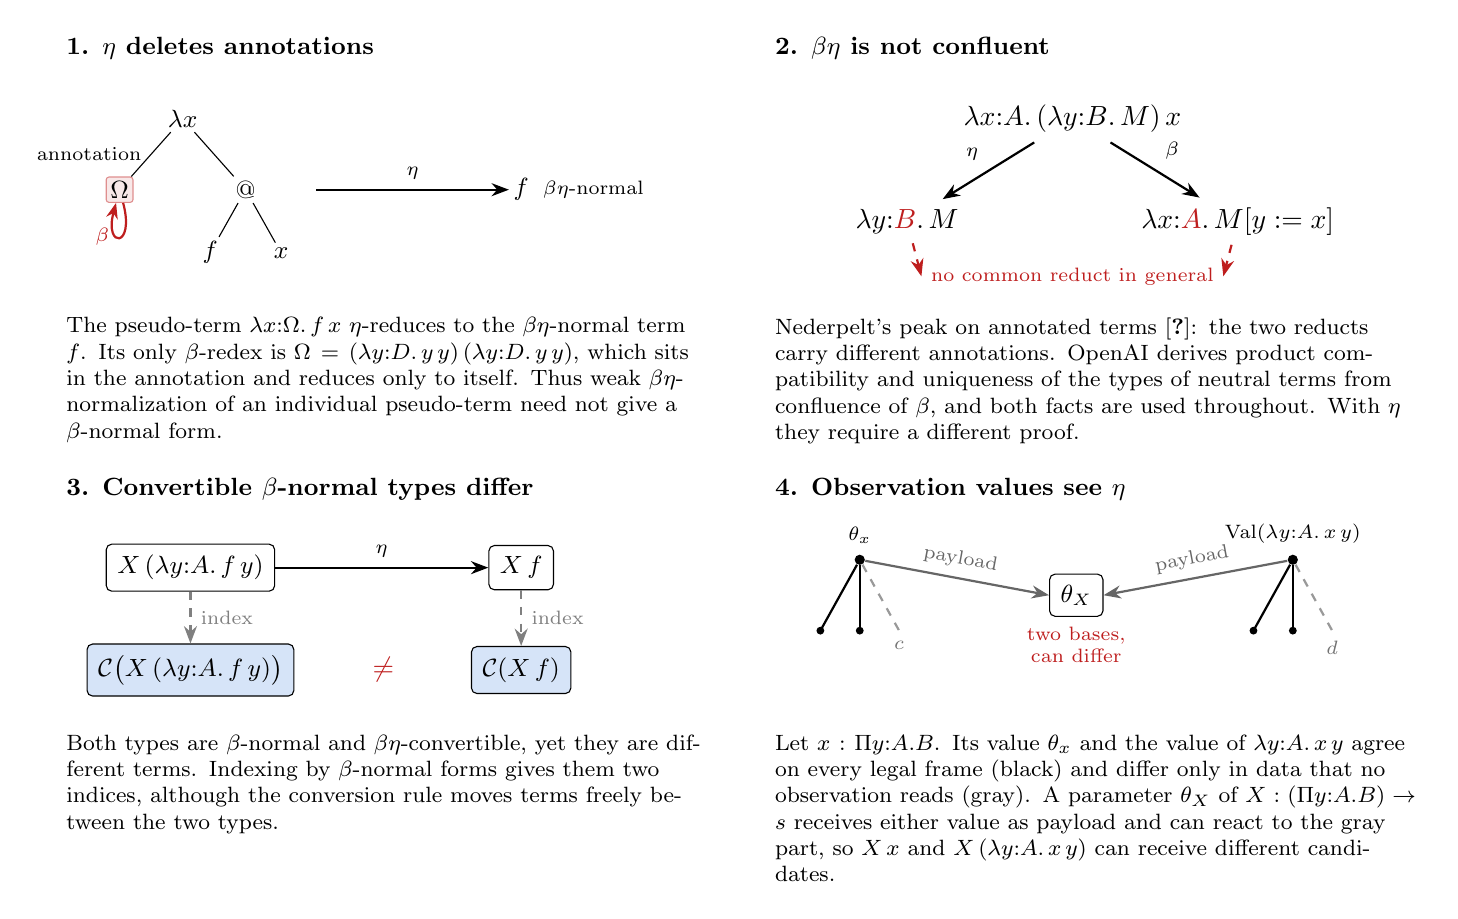
\begin{tikzpicture}[x=1cm,y=1cm]
% Panel 1. Eta deletes annotations.
\begin{scope}
\node[font=\small\bfseries,anchor=west] at (-0.3,1.0) {1. $\eta$ deletes annotations};
\node[tn] (lam) at (1.3,0.1) {$\lambda x$};
\node[ann] (om) at (0.5,-0.8) {$\Omega$};
\node[tn] (ap) at (2.1,-0.8) {$@$};
\node[tn] (f) at (1.65,-1.6) {$f$};
\node[tn] (x) at (2.55,-1.6) {$x$};
\draw (lam) -- node[lbl,left] {annotation} (om);
\draw (lam) -- (ap); \draw (ap) -- (f); \draw (ap) -- (x);
\draw[thick,warn,-{Stealth[length=2mm]}] (om) to[loop below,min distance=6mm]
  node[lbl,left] {$\beta$} (om);
\node[tn] (fr) at (5.6,-0.8) {$f$};
\draw[arr] (3.0,-0.8) -- node[lbl,above] {$\eta$} (fr);
\node[lbl,anchor=west] at (fr.east) {$\beta\eta$-normal};
\node[expl] at (-0.3,-2.3)
  {The pseudo-term $\lambda x{:}\Omega.\,f\,x$ $\eta$-reduces to the $\beta\eta$-normal term $f$. Its only
   $\beta$-redex is $\Omega=(\lambda y{:}D.\,y\,y)\,(\lambda y{:}D.\,y\,y)$, which sits in
   the annotation and reduces only to itself. Thus weak $\beta\eta$-normalization of
   an individual pseudo-term need not give a $\beta$-normal form.};
\end{scope}
% Panel 2. Nederpelt's peak.
\begin{scope}[xshift=9.0cm]
\node[font=\small\bfseries,anchor=west] at (-0.3,1.0) {2. $\beta\eta$ is not confluent};
\node (top) at (3.6,0.1) {$\lambda x{:}A.\,(\lambda y{:}B.\,M)\,x$};
\node (l) at (1.5,-1.2) {$\lambda y{:}\textcolor{warn}{B}.\,M$};
\node (r) at (5.7,-1.2) {$\lambda x{:}\textcolor{warn}{A}.\,M[y:=x]$};
\draw[arr] (top) -- node[lbl,above left] {$\eta$} (l);
\draw[arr] (top) -- node[lbl,above right] {$\beta$} (r);
\node[lbl,text=warn] (q) at (3.6,-1.9) {no common reduct in general};
\draw[arr,dashed,warn] (l) -- (q.west);
\draw[arr,dashed,warn] (r) -- (q.east);
\node[expl] at (-0.3,-2.3)
  {Nederpelt's peak on annotated terms~\cite{Nederpelt1973}: the two reducts carry
   different annotations. OpenAI derives product compatibility and uniqueness of the
   types of neutral terms from confluence of $\beta$, and both facts are used
   throughout. With $\eta$ they require a different proof.};
\end{scope}
% Panel 3. Convertible beta-normal types differ.
\begin{scope}[yshift=-5.6cm]
\node[font=\small\bfseries,anchor=west] at (-0.3,1.0) {3. Convertible $\beta$-normal types differ};
\node[box] (a) at (1.4,0) {$X\,(\lambda y{:}A.\,f\,y)$};
\node[box] (b) at (5.6,0) {$X\,f$};
\draw[arr] (a) -- node[lbl,above] {$\eta$} (b);
\node[box,fill=cand] (ca) at (1.4,-1.3) {$\mathcal C\bigl(X\,(\lambda y{:}A.\,f\,y)\bigr)$};
\node[box,fill=cand] (cb) at (5.6,-1.3) {$\mathcal C(X\,f)$};
\draw[arr,dashed,black!50] (a) -- node[lbl,right] {index} (ca);
\draw[arr,dashed,black!50] (b) -- node[lbl,right] {index} (cb);
\node[text=warn] at (3.85,-1.3) {$\neq$};
\node[expl] at (-0.3,-2.0)
  {Both types are $\beta$-normal and $\beta\eta$-convertible, yet they are different
   terms. Indexing by $\beta$-normal forms gives them two indices, although the conversion
   rule moves terms freely between the two types.};
\end{scope}
% Panel 4. The observation interpretation sees eta.
\begin{scope}[xshift=9.0cm,yshift=-5.6cm]
\node[font=\small\bfseries,anchor=west] at (-0.3,1.0) {4. Observation values see $\eta$};
\pic (A) at (0.9,0.1) {fan={$\theta_x$}{$c$}};
\pic (B) at (6.4,0.1) {fan={$\Val(\lambda y{:}A.\,x\,y)$}{$d$}};
\node[box] (tX) at (3.65,-0.35) {$\theta_X$};
\draw[arr,black!60] (A-r) -- node[lbl,above,sloped] {payload} (tX.west);
\draw[arr,black!60] (B-r) -- node[lbl,above,sloped] {payload} (tX.east);
\node[lbl,text=warn,align=center,anchor=north] at (tX.south) {two bases,\\ can differ};
\node[expl] at (-0.3,-2.0)
  {Let $x:\Pi y{:}A.B$. Its value $\theta_x$ and the value of $\lambda y{:}A.\,x\,y$ agree
   on every legal frame (black) and differ only in data that no observation reads
   (gray). A parameter $\theta_X$ of $X:(\Pi y{:}A.B)\to s$ receives either value as
   payload and can react to the gray part, so $X\,x$ and $X\,(\lambda y{:}A.\,x\,y)$
   can receive different candidates.};
\end{scope}
\end{tikzpicture}
\caption{The four places where the $\beta$ proof relies on something that fails with
$\eta$. Points~1 to~3 concern syntax and are repaired by the hypothesis (E),
skeletons and keys (Figures~\ref{fig:keys} and~\ref{fig:E}). Point~4 concerns the
semantic construction of case~3 and requires a new idea (Figure~\ref{fig:canon}).}
\label{fig:eta-breaks}
\end{figure}

\begin{figure}[H]
\centering
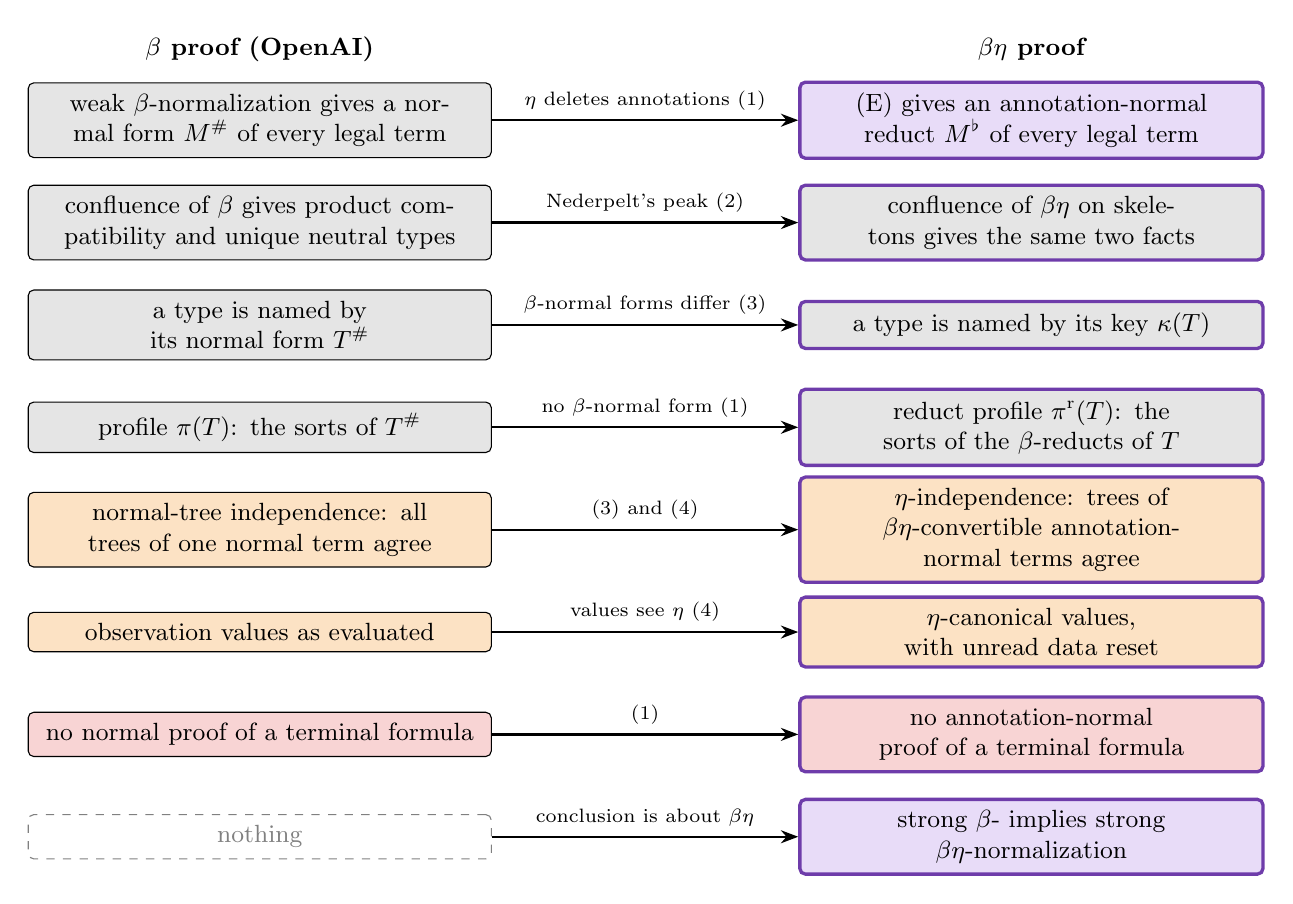
\begin{tikzpicture}[x=1cm,y=1cm]
\node[font=\small\bfseries] at (-4.9,0.9) {$\beta$ proof (OpenAI)};
\node[font=\small\bfseries] at (4.9,0.9) {$\beta\eta$ proof};
% Row 1
\node[box,fill=shared,text width=5.6cm] (l1) at (-4.9,0)
  {weak $\beta$-normalization gives a normal form $M^\#$ of every legal term};
\node[newbox,fill=etanew,text width=5.6cm] (r1) at (4.9,0)
  {(E) gives an annotation-normal reduct $M^\flat$ of every legal term};
\draw[arr] (l1) -- node[lbl,above] {$\eta$ deletes annotations (1)} (r1);
% Row 2
\node[box,fill=shared,text width=5.6cm] (l2) at (-4.9,-1.3)
  {confluence of $\beta$ gives product compatibility and unique neutral types};
\node[newbox,fill=shared,text width=5.6cm] (r2) at (4.9,-1.3)
  {confluence of $\beta\eta$ on skeletons gives the same two facts};
\draw[arr] (l2) -- node[lbl,above] {Nederpelt's peak (2)} (r2);
% Row 3
\node[box,fill=shared,text width=5.6cm] (l3) at (-4.9,-2.6)
  {a type is named by its normal form $T^\#$};
\node[newbox,fill=shared,text width=5.6cm] (r3) at (4.9,-2.6)
  {a type is named by its key $\kappa(T)$};
\draw[arr] (l3) -- node[lbl,above] {$\beta$-normal forms differ (3)} (r3);
% Row 4
\node[box,fill=shared,text width=5.6cm] (l4) at (-4.9,-3.9)
  {profile $\pi(T)$: the sorts of $T^\#$};
\node[newbox,fill=shared,text width=5.6cm] (r4) at (4.9,-3.9)
  {reduct profile $\pi^{\mathrm r}(T)$: the sorts of the $\beta$-reducts of $T$};
\draw[arr] (l4) -- node[lbl,above] {no $\beta$-normal form (1)} (r4);
% Row 5
\node[box,fill=obs,text width=5.6cm] (l5) at (-4.9,-5.2)
  {normal-tree independence: all trees of one normal term agree};
\node[newbox,fill=obs,text width=5.6cm] (r5) at (4.9,-5.2)
  {$\eta$-independence: trees of $\beta\eta$-convertible annotation-normal terms agree};
\draw[arr] (l5) -- node[lbl,above] {(3) and (4)} (r5);
% Row 6
\node[box,fill=obs,text width=5.6cm] (l6) at (-4.9,-6.5)
  {observation values as evaluated};
\node[newbox,fill=obs,text width=5.6cm] (r6) at (4.9,-6.5)
  {$\eta$-canonical values, with unread data reset};
\draw[arr] (l6) -- node[lbl,above] {values see $\eta$ (4)} (r6);
% Row 7
\node[box,fill=par,text width=5.6cm] (l7) at (-4.9,-7.8)
  {no normal proof of a terminal formula};
\node[newbox,fill=par,text width=5.6cm] (r7) at (4.9,-7.8)
  {no annotation-normal proof of a terminal formula};
\draw[arr] (l7) -- node[lbl,above] {(1)} (r7);
% Row 8
\node[box,dashed,draw=black!50,text=black!50,text width=5.6cm] (l8) at (-4.9,-9.1)
  {nothing};
\node[newbox,fill=etanew,text width=5.6cm] (r8) at (4.9,-9.1)
  {strong $\beta$- implies strong $\beta\eta$-normalization};
\draw[arr] (l8) -- node[lbl,above] {conclusion is about $\beta\eta$} (r8);
\end{tikzpicture}
\caption{What the $\beta\eta$ proof replaces. Each row pairs an ingredient of the
$\beta$ proof with its replacement, and the arrow names the point of
Figure~\ref{fig:eta-breaks} that forces the change. Every other part of the
$\beta$ proof is reused as it stands.}
\label{fig:replace}
\end{figure}

\paragraph{Skeletons and keys.} OpenAI uses the normal form of a type as its name.
With $\eta$, however, convertible $\beta$-normal types can differ, and weak
$\beta\eta$-normalization of an individual pseudo-term need not give a
$\beta$-normal form. The $\beta\eta$ proof therefore names a type by its key.
Keys are computed from skeletons, on which $\beta\eta$ is confluent again
(Figure~\ref{fig:keys}).

\begin{figure}[H]
\centering
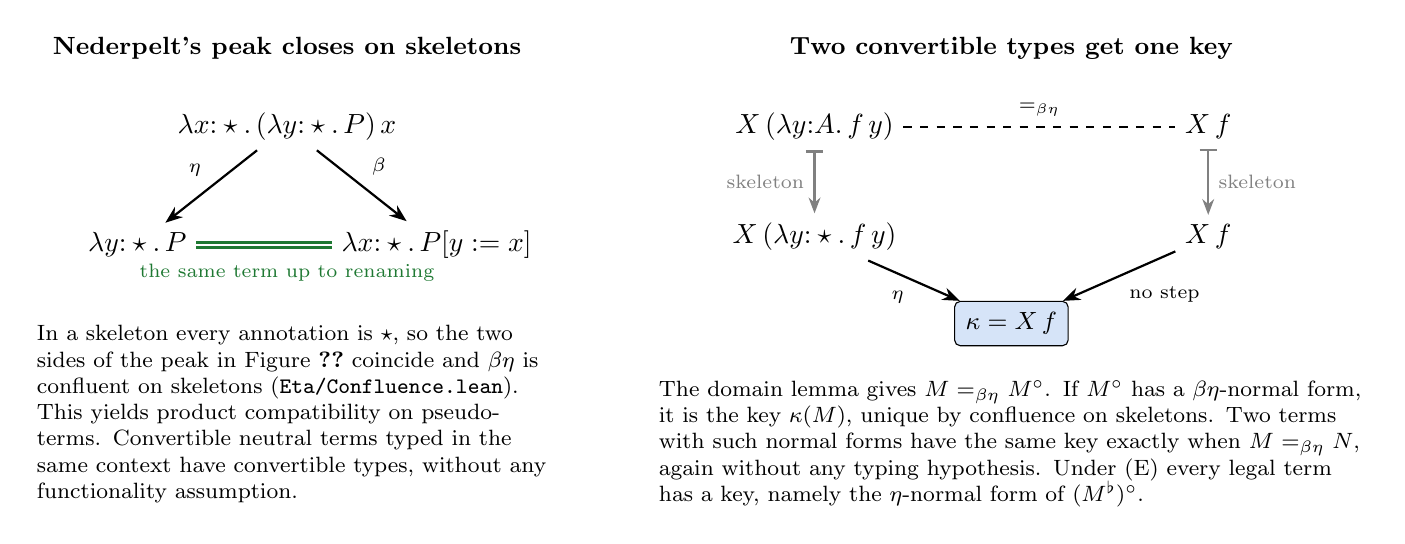
\begin{tikzpicture}[x=1cm,y=1cm]
\begin{scope}
\node[font=\small\bfseries] at (2.4,1.0) {Nederpelt's peak closes on skeletons};
\node (top) at (2.4,0) {$\lambda x{:}\star.\,(\lambda y{:}\star.\,P)\,x$};
\node (l) at (0.5,-1.5) {$\lambda y{:}\star.\,P$};
\node (r) at (4.3,-1.5) {$\lambda x{:}\star.\,P[y:=x]$};
\draw[arr] (top) -- node[lbl,above left] {$\eta$} (l);
\draw[arr] (top) -- node[lbl,above right] {$\beta$} (r);
\draw[double,very thick,okgreen] (l) -- (r);
\node[lbl,text=okgreen] at (2.4,-1.85) {the same term up to renaming};
\node[expl,text width=6.6cm] at (-0.9,-2.4)
  {In a skeleton every annotation is $\star$, so the two sides of the peak in
   Figure~\ref{fig:eta-breaks} coincide and $\beta\eta$ is confluent on skeletons
   (\texttt{Eta/Confluence.lean}). This yields product compatibility on pseudo-terms.
   Convertible neutral terms typed in the same context have convertible types,
   without any functionality assumption.};
\end{scope}
\begin{scope}[xshift=7.4cm]
\node[font=\small\bfseries] at (4.2,1.0) {Two convertible types get one key};
\node (M) at (1.7,0) {$X\,(\lambda y{:}A.\,f\,y)$};
\node (N) at (6.7,0) {$X\,f$};
\draw[thick,dashed] (M) -- node[lbl,above] {$\eqbe$} (N);
\node (Ms) at (1.7,-1.4) {$X\,(\lambda y{:}\star.\,f\,y)$};
\node (Ns) at (6.7,-1.4) {$X\,f$};
\draw[mapsto] (M) -- node[lbl,left] {skeleton} (Ms);
\draw[mapsto] (N) -- node[lbl,right] {skeleton} (Ns);
\node[box,fill=cand] (k) at (4.2,-2.5) {$\kappa=X\,f$};
\draw[arr] (Ms) -- node[lbl,below left] {$\eta$} (k);
\draw[arr] (Ns) -- node[lbl,below right] {no step} (k);
\node[expl,text width=9.0cm] at (-0.4,-3.1)
  {The domain lemma gives $M\eqbe M^\circ$. If $M^\circ$ has a $\beta\eta$-normal form,
   it is the key $\kappa(M)$, unique by confluence on skeletons.
   Two terms with such normal forms have the same key exactly when $M\eqbe N$, again
   without any typing hypothesis. Under (E) every legal term has a key, namely the
   $\eta$-normal form of $(M^\flat)^\circ$.};
\end{scope}
\end{tikzpicture}
\caption{Skeletons repair point~2 and keys repair point~3 of
Figure~\ref{fig:eta-breaks}. In the example of point~3 both types have key $X\,f$.
Product domains are kept in the skeleton, because typing inspects them and $\eta$
never deletes them.}
\label{fig:keys}
\end{figure}

\paragraph{The hypothesis (E).} OpenAI's argument normalizes legal terms in a few
places: actual types, argument keys, substituted types and the paradox. With $\eta$
the construction uses annotation-normal reducts (Figure~\ref{fig:E}). Each of
these uses was checked to work with such reducts, for the same reason every time:
the argument inspects $\lambda$-bodies and application spines, but never
$\lambda$-annotations.

\begin{figure}[H]
\centering
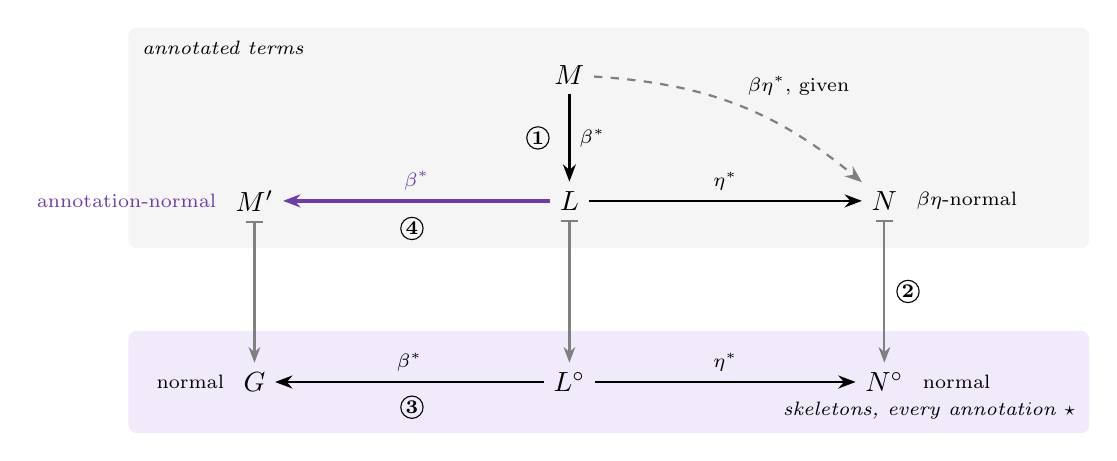
\begin{tikzpicture}[x=1cm,y=1cm]
\fill[black!4,rounded corners=3pt] (-1.6,-0.6) rectangle (10.6,2.2);
\fill[etanew!60,rounded corners=3pt] (-1.6,-2.95) rectangle (10.6,-1.65);
\node[lbl,font=\scriptsize\itshape,anchor=north west] at (-1.55,2.15) {annotated terms};
\node[lbl,font=\scriptsize\itshape,anchor=south east] at (10.55,-2.9)
  {skeletons, every annotation $\star$};
\node (M) at (4,1.6) {$M$};
\node (L) at (4,0) {$L$};
\node (N) at (8,0) {$N$};
\node (Mp) at (0,0) {$M'$};
\node (Ls) at (4,-2.3) {$L^\circ$};
\node (Ns) at (8,-2.3) {$N^\circ$};
\node (G) at (0,-2.3) {$G$};
\node[lbl,anchor=west] at (N.east) {$\beta\eta$-normal};
\node[lbl,anchor=west] at (Ns.east) {normal};
\node[lbl,anchor=east] at (G.west) {normal};
\node[lbl,anchor=east,text=etaline] at (Mp.west) {annotation-normal};
\draw[arr,dashed,black!50] (M) to[bend left=18]
  node[lbl,above right,text=black] {$\beta\eta^*$, given} (N);
\draw[arr] (M) -- node[lbl,right] {$\beta^*$} (L);
\draw[arr] (L) -- node[lbl,above] {$\eta^*$} (N);
\draw[arr] (Ls) -- node[lbl,above] {$\eta^*$} (Ns);
\draw[arr] (Ls) -- node[lbl,above] {$\beta^*$} (G);
\draw[arr,very thick,etaline] (L) -- node[lbl,above] {$\beta^*$} (Mp);
\draw[mapsto] (L) -- (Ls);
\draw[mapsto] (N) -- (Ns);
\draw[mapsto] (Mp) -- (G);
\node[stepc] at (3.6,0.8) {1};
\node[stepc] at (8.3,-1.15) {2};
\node[stepc] at (2.0,-2.62) {3};
\node[stepc] at (2.0,-0.35) {4};
\end{tikzpicture}

\smallskip
\begin{minipage}{0.92\linewidth}\footnotesize
\stepn{1} $\eta$-postponement~\cite{Takahashi1995} moves all $\eta$-steps of the given
sequence to its end.
\stepn{2} Erasing annotations either keeps an $\eta$-step or makes it trivial, and
$N^\circ$ is normal because $N$ is.
\stepn{3} A skeleton that $\eta$-reduces to a normal term is weakly
$\beta$-normalizing. Here the skeleton matters: since all annotations are $\star$,
Nederpelt's peak cannot occur.
\stepn{4} Every $\beta$-step of a skeleton comes from a $\beta$-step of the term, so
$L^\circ\to_\beta^* G$ lifts to $L\to_\beta^* M'$ with $M'^\circ=G$. A term with a
normal skeleton is annotation-normal.
\end{minipage}
\caption{From weak $\beta\eta$-normalization to (E). This step requires no normality
of the annotations of $M'$. For arbitrary pseudo-terms they may diverge, as in
$\lambda x{:}\Omega.\,f\,x$.}
\label{fig:E}
\end{figure}

\paragraph{Substitution.} Substitution is where the $\beta$ proof depends most on
normal forms. The codomain $E[x:=n]$ of a product is not a subterm of the product,
so OpenAI normalizes it again, and uniqueness of normal forms makes the result
canonical. Figure~\ref{fig:subst} shows what happens with $\eta$. Panel~(a) shows
that substitution produces $\eta$-variants of the same type. Panel~(b) depicts the
specialization law of the interface, which substitutes an argument into a codomain,
as a square that closes in the $\beta$ proof but only up to $\beta\eta$ in the
$\beta\eta$ proof.

\begin{figure}[H]
\centering
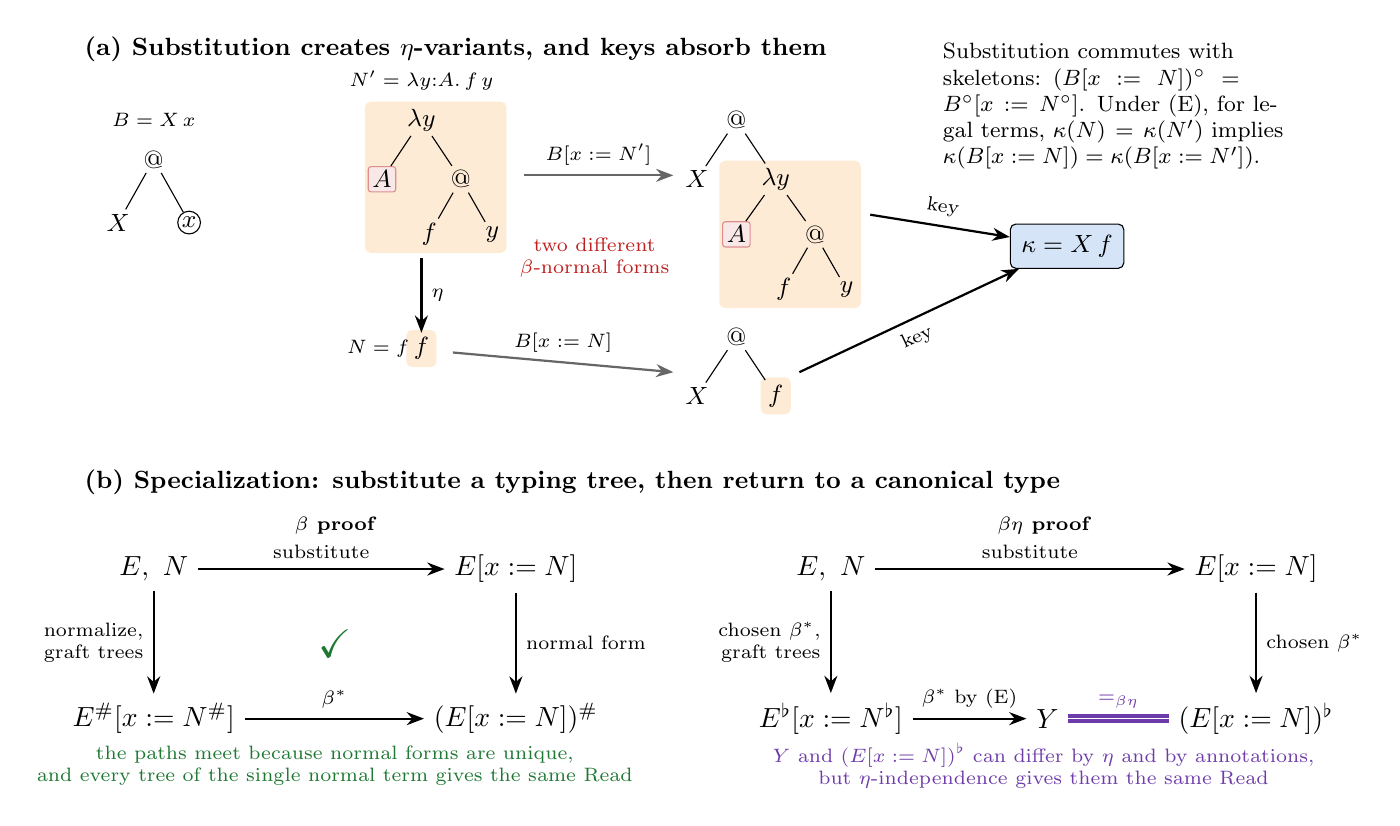
\begin{tikzpicture}[x=1cm,y=1cm]
\node[font=\small\bfseries,anchor=west] at (-1.0,1.9)
  {(a) Substitution creates $\eta$-variants, and keys absorb them};
% The type B = X x with its hole x.
\node[lbl] at (0,1.0) {$B=X\,x$};
\node[tn] (b) at (0,0.5) {$@$};
\node[tn] (bX) at (-0.45,-0.3) {$X$};
\node[tn,draw,circle,inner sep=0.6pt] (bx) at (0.45,-0.3) {$x$};
\draw (b) -- (bX); \draw (b) -- (bx);
% The two arguments.
\node[lbl] at (3.4,1.5) {$N'=\lambda y{:}A.\,f\,y$};
\node[tn] (n1) at (3.4,1.0) {$\lambda y$};
\node[ann] (n1A) at (2.9,0.25) {$A$};
\node[tn] (n1a) at (3.9,0.25) {$@$};
\node[tn] (n1f) at (3.5,-0.45) {$f$};
\node[tn] (n1y) at (4.3,-0.45) {$y$};
\draw (n1) -- (n1A); \draw (n1) -- (n1a); \draw (n1a) -- (n1f); \draw (n1a) -- (n1y);
\node[lbl] at (2.85,-1.9) {$N=f$};
\node[tn] (n2) at (3.4,-1.9) {$f$};
\draw[arr] (3.4,-0.75) -- node[lbl,right] {$\eta$} (n2);
% The two results, with the grafted subtree shaded.
\node[tn] (r1) at (7.4,1.0) {$@$};
\node[tn] (r1X) at (6.9,0.25) {$X$};
\node[tn] (r1l) at (7.9,0.25) {$\lambda y$};
\node[ann] (r1A) at (7.4,-0.45) {$A$};
\node[tn] (r1a) at (8.4,-0.45) {$@$};
\node[tn] (r1f) at (8.0,-1.15) {$f$};
\node[tn] (r1y) at (8.8,-1.15) {$y$};
\draw (r1) -- (r1X); \draw (r1) -- (r1l); \draw (r1l) -- (r1A); \draw (r1l) -- (r1a);
\draw (r1a) -- (r1f); \draw (r1a) -- (r1y);
\node[tn] (r2) at (7.4,-1.75) {$@$};
\node[tn] (r2X) at (6.9,-2.5) {$X$};
\node[tn] (r2f) at (7.9,-2.5) {$f$};
\draw (r2) -- (r2X); \draw (r2) -- (r2f);
\begin{scope}[on background layer]
\node[fit=(r1l)(r1A)(r1f)(r1y),fill=obs!70,rounded corners=2pt,inner sep=1pt] {};
\node[fit=(r2f),fill=obs!70,rounded corners=2pt,inner sep=1pt] {};
\node[fit=(n1)(n1A)(n1f)(n1y),fill=obs!70,rounded corners=2pt,inner sep=1pt] {};
\node[fit=(n2),fill=obs!70,rounded corners=2pt,inner sep=1pt] {};
\end{scope}
\draw[arr,black!60] (4.7,0.3) -- node[lbl,above,text=black] {$B[x:=N']$} (6.6,0.3);
\draw[arr,black!60] (3.8,-1.95) -- node[lbl,above,text=black] {$B[x:=N]$} (6.6,-2.2);
\node[lbl,text=warn,align=center] at (5.6,-0.75) {two different\\ $\beta$-normal forms};
\node[box,fill=cand] (k) at (11.6,-0.6) {$\kappa=X\,f$};
\draw[arr] (9.1,-0.2) -- node[lbl,above,sloped] {key} (k);
\draw[arr] (8.2,-2.2) -- node[lbl,below,sloped] {key} (k);
\node[expl,text width=4.6cm] at (9.9,2.1)
  {Substitution commutes with skeletons: $(B[x:=N])^\circ=B^\circ[x:=N^\circ]$.
   Under (E), for legal terms, $\kappa(N)=\kappa(N')$ implies
   $\kappa(B[x:=N])=\kappa(B[x:=N'])$.};
% Panel (b). Specialization.
\node[font=\small\bfseries,anchor=west] at (-1.0,-3.6)
  {(b) Specialization: substitute a typing tree, then return to a canonical type};
\begin{scope}[yshift=-4.7cm]
\node[lbl,font=\scriptsize\bfseries] at (2.3,0.55) {$\beta$ proof};
\node (tl) at (0,0) {$E,\ N$};
\node (tr) at (4.6,0) {$E[x:=N]$};
\node (bl) at (0,-1.9) {$E^\#[x:=N^\#]$};
\node (br) at (4.6,-1.9) {$(E[x:=N])^\#$};
\draw[arr] (tl) -- node[lbl,above] {substitute} (tr);
\draw[arr] (tl) -- node[lbl,left,align=right] {normalize,\\ graft trees} (bl);
\draw[arr] (tr) -- node[lbl,right] {normal form} (br);
\draw[arr] (bl) -- node[lbl,above] {$\beta^*$} (br);
\node[text=okgreen] at (2.3,-0.95) {\Large$\checkmark$};
\node[lbl,text=okgreen,align=center] at (2.3,-2.5)
  {the paths meet because normal forms are unique,\\ and every tree of the single
   normal term gives the same Read};
\end{scope}
\begin{scope}[xshift=8.6cm,yshift=-4.7cm]
\node[lbl,font=\scriptsize\bfseries] at (2.7,0.55) {$\beta\eta$ proof};
\node (tl) at (0,0) {$E,\ N$};
\node (tr) at (5.4,0) {$E[x:=N]$};
\node (bl) at (0,-1.9) {$E^\flat[x:=N^\flat]$};
\node (X) at (2.75,-1.9) {$Y$};
\node (br) at (5.4,-1.9) {$(E[x:=N])^\flat$};
\draw[arr] (tl) -- node[lbl,above] {substitute} (tr);
\draw[arr] (tl) -- node[lbl,left,align=right] {chosen $\beta^*$,\\ graft trees} (bl);
\draw[arr] (tr) -- node[lbl,right] {chosen $\beta^*$} (br);
\draw[arr] (bl) -- node[lbl,above] {$\beta^*$ by (E)} (X);
\draw[double,very thick,etaline] (X) -- node[lbl,above,text=etaline] {$\eqbe$} (br);
\node[lbl,text=etaline,align=center] at (2.7,-2.5)
  {$Y$ and $(E[x:=N])^\flat$ can differ by $\eta$ and by annotations,\\
   but $\eta$-independence gives them the same Read};
\end{scope}
\end{tikzpicture}
\caption{Substitution with and without $\eta$. (a)~Arguments that are equal up to
$\eta$ yield two different $\beta$-normal types, $X\,(\lambda y{:}A.\,f\,y)$ and $X\,f$,
which the $\beta$ proof would treat as two indices, although their keys are equal.
(b)~The tree of the argument is grafted into the tree of the codomain at $x$, with
the value of the argument as payload. In the $\beta\eta$ proof this value is
canonical, so the new variable clause reads it unchanged. The square closes exactly
in the $\beta$ proof, and in the $\beta\eta$ proof it closes only up to $\beta\eta$,
by $\eta$-independence (Figure~\ref{fig:canon}).}
\label{fig:subst}
\end{figure}

\paragraph{$\eta$-canonical values.} Point~4 is the only substantive change. A value
in case~3 is a table indexed by frames, and evaluation reads only part of this table.
The proof defines a canonical form $\canon_T(w)$ that keeps the part that is read
and resets the rest (\texttt{canonValue}), and a variable now evaluates to the
canonical form of its parameter. Two laws then make $\eta$ hold exactly for values:
application commutes with $\canon$, and
$\Lam\bigl((k,p)\mapsto\canon(\App(w,k,\canon\,p))\bigr)=\canon(w)$ whenever $T$ is
not a sort (\texttt{lambdaValue\_eta}). Moreover, every evaluated value is canonical
(\texttt{preEvaluate\_canonical}). Figure~\ref{fig:canon} shows the definition and
the one new case of the invariance lemma.

\begin{figure}[H]
\centering
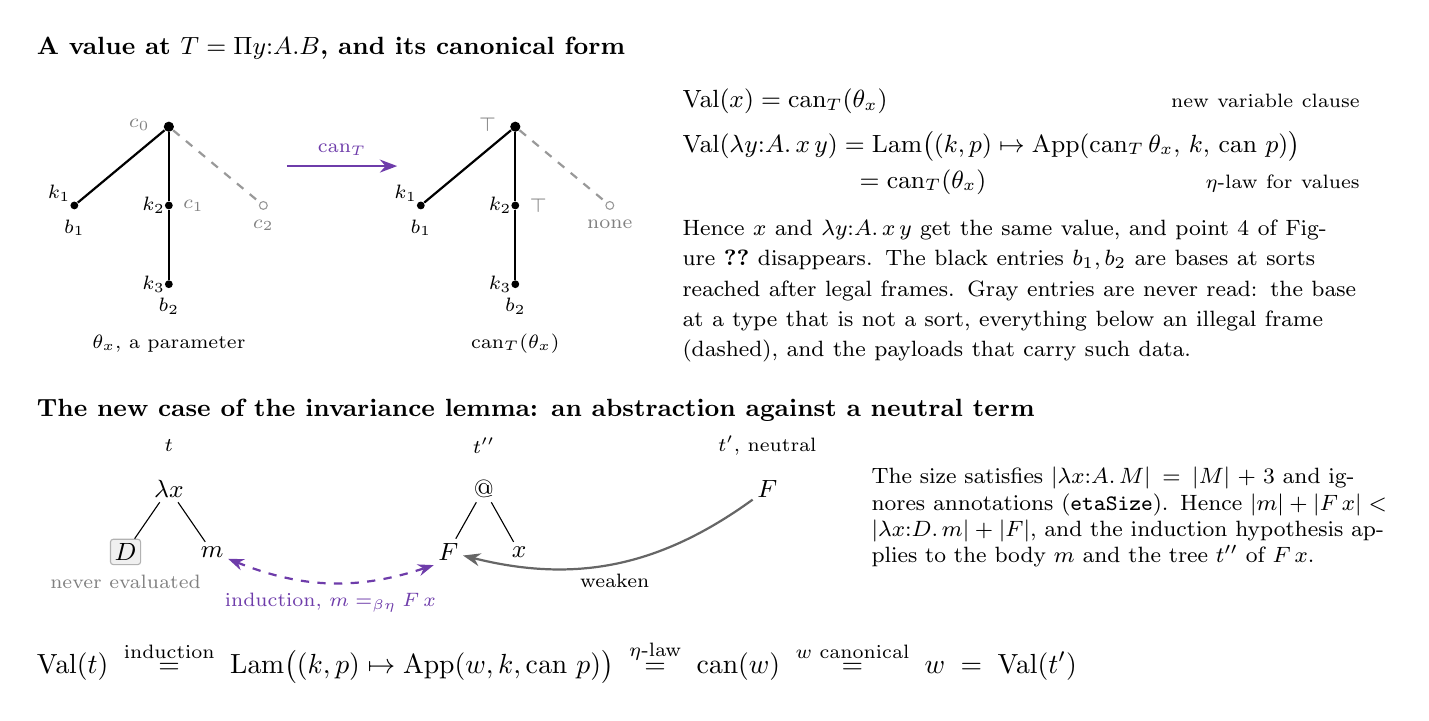
\begin{tikzpicture}[x=1cm,y=1cm]
\node[font=\small\bfseries,anchor=west] at (-1.8,1.0) {A value at $T=\Pi y{:}A.B$, and its canonical form};
\pic (V) at (0,0) {vtree={$c_0$}{$c_1$}{$c_2$}};
\node[lbl] at (0,-2.75) {$\theta_x$, a parameter};
\pic (W) at (4.4,0) {vtree={$\top$}{$\top$}{none}};
\node[lbl] at (4.4,-2.75) {$\canon_T(\theta_x)$};
\draw[arr,etaline] (1.5,-0.5) -- node[lbl,above,text=etaline] {$\canon_T$} (2.9,-0.5);
\node[font=\small,text width=8.6cm,align=left,anchor=north west] at (6.4,0.6)
  {$\Val(x)=\canon_T(\theta_x)$ \hfill {\scriptsize new variable clause}\\[5pt]
   $\Val(\lambda y{:}A.\,x\,y)
     =\Lam\bigl((k,p)\mapsto\App(\canon_T\theta_x,\,k,\,\canon\,p)\bigr)$\\[2pt]
   \hspace*{2.25cm}$=\canon_T(\theta_x)$ \hfill {\scriptsize $\eta$-law for values}\\[6pt]
   {\footnotesize Hence $x$ and $\lambda y{:}A.\,x\,y$ get the same value, and point~4
   of Figure~\ref{fig:eta-breaks} disappears. The black entries $b_1,b_2$ are bases at
   sorts reached after legal frames. Gray entries are never read: the base at a type
   that is not a sort, everything below an illegal frame (dashed), and the payloads
   that carry such data.}};
% The eta case of eta-independence.
\node[font=\small\bfseries,anchor=west] at (-1.8,-3.6)
  {The new case of the invariance lemma: an abstraction against a neutral term};
\begin{scope}[yshift=-4.6cm]
\node[lbl] at (0,0.55) {$t$};
\node[tn] (tl) at (0,0) {$\lambda x$};
\node[ann,fill=black!6,draw=black!30] (tD) at (-0.55,-0.8) {$D$};
\node[tn] (tm) at (0.55,-0.8) {$m$};
\draw (tl) -- (tD); \draw (tl) -- (tm);
\node[lbl,text=black!50,anchor=north] at (tD.south) {never evaluated};
\node[lbl] at (4.0,0.55) {$t''$};
\node[tn] (ta) at (4.0,0) {$@$};
\node[tn] (taF) at (3.55,-0.8) {$F$};
\node[tn] (tax) at (4.45,-0.8) {$x$};
\draw (ta) -- (taF); \draw (ta) -- (tax);
\node[lbl] at (7.6,0.55) {$t'$, neutral};
\node[tn] (tF) at (7.6,0) {$F$};
\draw[arr,black!60] (tF) to[bend left=25] node[lbl,below,text=black] {weaken} (taF);
\draw[{Stealth[length=2mm]}-{Stealth[length=2mm]},thick,dashed,etaline] (tm) to[bend right=20]
  node[lbl,below,text=etaline] {induction, $m\eqbe F\,x$} (taF.south west);
\node[expl,text width=6.6cm] at (8.8,0.4)
  {The size satisfies $|\lambda x{:}A.\,M|=|M|+3$ and ignores annotations
   (\texttt{etaSize}). Hence $|m|+|F\,x|<|\lambda x{:}D.\,m|+|F|$, and the induction
   hypothesis applies to the body $m$ and the tree $t''$ of $F\,x$.};
\node[anchor=west] at (-1.8,-2.2)
  {$\displaystyle
   \Val(t)\;\overset{\text{induction}}{=}\;
   \Lam\bigl((k,p)\mapsto\App(w,k,\canon\,p)\bigr)\;\overset{\eta\text{-law}}{=}\;
   \canon(w)\;\overset{w\text{ canonical}}{=}\;w\;=\;\Val(t')$};
\end{scope}
\end{tikzpicture}
\caption{$\eta$-canonical values. Top: canonicalization keeps what observations read
and resets the rest, and with the new variable clause $x$ and $\lambda y{:}A.\,x\,y$
receive the same value. Bottom: the $\eta$-case of the lemma that replaces OpenAI's
normal-tree independence (\texttt{eta\_case} in \texttt{EtaIndependence.lean}), where
$w=\Val(t')$. Since annotations are never evaluated, the cases of two abstractions
and of two neutral terms go through as in OpenAI's proof.}
\label{fig:canon}
\end{figure}

\paragraph{What stays the same.} The recursion over components, the three cases, the
profile graph and the paradox are OpenAI's. Reduct profiles of
$\mathrm{PTS}_{\beta\eta}$ are feasible profiles of OpenAI's graph, so the same graph
decides the case split. In particular, Table~\ref{tab:systems} and the
counterexamples and counts of Section~\ref{sec:reduce} apply to
$\mathrm{PTS}_{\beta\eta}$ without change. The $\beta\eta$ proof is not shorter than
the $\beta$ proof (Figure~\ref{fig:sizes-be}). Rather, it is a complete check that
OpenAI's argument survives the weaker hypothesis (E), together with one new idea,
the $\eta$-canonical values.

\begin{figure}[H]
\centering
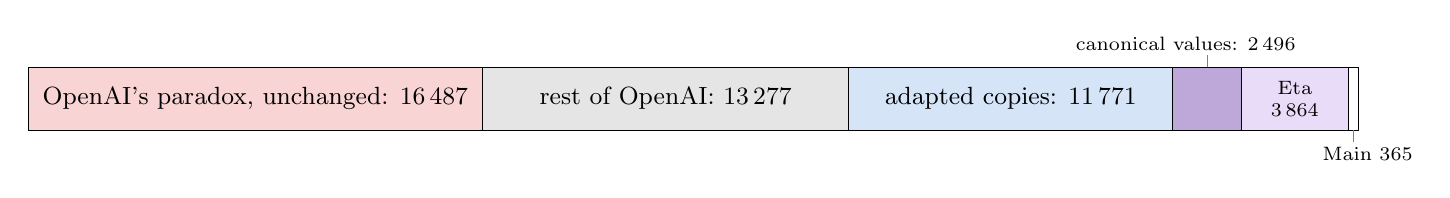
\begin{tikzpicture}[x=0.35mm,y=1cm]
% One unit is 100 lines. The whole bar is 48 260 lines.
\fill[par] (0,0) rectangle (164.87,0.8);
\fill[shared] (164.87,0) rectangle (297.64,0.8);
\fill[cand] (297.64,0) rectangle (415.35,0.8);
\fill[etaline!45] (415.35,0) rectangle (440.31,0.8);
\fill[etanew] (440.31,0) rectangle (478.95,0.8);
\fill[white] (478.95,0) rectangle (482.60,0.8);
\draw (0,0) rectangle (482.60,0.8);
\foreach \x in {164.87,297.64,415.35,440.31,478.95} \draw (\x,0) -- (\x,0.8);
\node[font=\small] at (82.4,0.4) {OpenAI's paradox, unchanged: 16\,487};
\node[font=\small] at (231.3,0.4) {rest of OpenAI: 13\,277};
\node[font=\small] at (356.5,0.4) {adapted copies: 11\,771};
\node[font=\scriptsize,align=center] at (459.6,0.4) {Eta\\3\,864};
\node[font=\scriptsize] at (420.0,1.1) {canonical values: 2\,496};
\draw[gray] (427.8,0.8) -- (427.8,0.95);
\node[font=\scriptsize] at (486.0,-0.3) {Main 365};
\draw[gray] (480.8,0) -- (480.8,-0.15);
\end{tikzpicture}
\caption{Lean lines of \texttt{PTS-beta-eta} by origin. The adapted copies are
OpenAI's candidate half, rewritten for keys and annotation-normal reducts. The two
violet slices are the $\eta$-specific files: \texttt{Canon}, \texttt{CanonLaws} and
\texttt{EtaIndependence}, and the directory \texttt{Eta}.}
\label{fig:sizes-be}
\end{figure}

\section*{Acknowledgements}
\begin{sloppypar}
The figures follow the argument and Lean formalization of OpenAI~\cite{OpenAI2026}
and the Lean development \texttt{PTS-beta-eta}~\cite{PTSbetaetaLean}, and cite the
corresponding Lean files throughout. This guide, its figures and the counts in
Section~\ref{sec:reduce} were prepared with the help of Claude Opus~5.5, used
through Claude Code.
\end{sloppypar}

\bibliographystyle{plain}
{\small
\bibliography{references}
}

\end{document}
